\documentclass[11pt,twoside,a4paper]{book}  
% definice dokumentu
\usepackage[czech, english]{babel}
\usepackage[T1]{fontenc} 				% pouzije EC fonty 
\usepackage[utf8]{inputenc} 			% utf8 kódování vstupu 
\usepackage[square, numbers]{natbib}	% sazba pouzite literatury
\usepackage{indentfirst} 				% 1. odstavec jako v cestine, pro práci v aj možno zakomentovat
\usepackage{fancyhdr}					% tisk hlaviček a patiček stránek
\usepackage{nomencl} 					% umožňuje snadno definovat zkratky a jejich seznam

%%%%%%%%%%%%%%%%%%%%%%%%%%%%%%%%%%%%%%%%%%%%%%%%%%%%%%%%%%%%%%%
% informace o práci
\newcommand\WorkTitle{Kalibrační a ovládací software sítě částicových pixelových detektorů umístěných uvnitř experimentu ATLAS na~LHC~v~CERN} % název
\newcommand\FirstandFamilyName{Jakub Begera} % autor
\newcommand\Supervisor{Ing. Štěpán Polanský} % vedoucí

\newcommand\TypeOfWork{Bakalářská práce}	% typ práce [Diplomová práce | Bakalářská práce | Bachelor's Project | Master's Thesis ]	

% Nastavte následují podle vašeho oboru a programu (pomoc hledejte na http://www.fel.cvut.cz/cz/education/bk/prehled.html)								
\newcommand\StudProgram{Otevřená informatika, Bakalářský} % program
\newcommand\StudBranch{Softwarové systémy} % obor

%%%%%%%%%%%%%%%%%%%%%%%%%%%%%%%%%%%%%%%%%%%%%%%%%%%%%%%%%%%%%%%
% minimální importy
\usepackage{graphicx}					% pro vkládání obrázků
\usepackage{k336_thesis_macros} 		% specialni makra pro formatovani DP a BP
\usepackage[
pdftitle={\WorkTitle},				% nastaví v informacích o pdf název
pdfauthor={\FirstandFamilyName},	% nastaví v informacích o pdf autora
colorlinks=true,					% před tiskem doporučujeme nastavit na false, aby odkazy a url nebyly šedé při ČB tisku
breaklinks=true,
urlcolor=red,
citecolor=blue,
linkcolor=blue,
unicode=true,
]
{hyperref}								% pro zobrazování "prokliknutelných" linků 

% rozšiřující importy
\usepackage{listings} 			%slouží pro tisk zdrojových kódů se syntax higlighting
\usepackage{algorithmicx} 		%slouží pro zápis algoritmů
\usepackage{algpseudocode} 		%slouží pro výpis pseudokódu
\usepackage{inconsolata}		%monospace font
\usepackage{soul}				%zvýrazňovač
\usepackage[final]{pdfpages}    %PDF include
\usepackage{subcaption}			%pro reference na subfigures 

%%%%%%%%%%%%%%%%%%%%%%%%%%%%%%%%%%%%%%%%%%%%%%%%%%%%%%%%%%%%%%%
% příkazy šablony
\makenomenclature								% při překladu zajistí vytvoření pracovního souboru se seznamem zkratek

\let\oldUrl\url									% url adresy budou zobrazeny: <url> 
\renewcommand\url[1]{<\texttt{\oldUrl{#1}}>}

%%%%%%%%%%%%%%%%%%%%%%%%%%%%%%%%%%%%%%%%%%%%%%%%%%%%%%%%%%%%%%%
% vaše vlastní příkazy
\newcommand*{\nomExpl}[2]{#2 (#1)\nomenclature{#1}{#2}} % usnadňuje zápis zkratek : Slova ke Zkrácení (SZ)
\newcommand*{\nom}[2]{#1\nomenclature{#1}{#2}} % usnadňuje zápis zkratek : SZ
\newcommand*{\todo}{\hl{\textbf{TODO}}} % pro poznámky
\newcommand{\addbibresource}[1]{}


%%%%%%%%%%%%%%%%%%%%%%%%%%%%%%%%%%%%%%%%%%%%%%%%%%%%%%%%%%%%%%%
% vlastní dokument
%%%%%%%%%%%%%%%%%%%%%%%%%%%%%%%%%%%%%%%%%%%%%%%%%%%%%%%%%%%%%%%
\begin{document}

	%%%%%%%%%%%%%%%%%%%%%%%%%% 
	% nastavení jazyka, kterým je práce psána
	\selectlanguage{czech}	% podle jazyka práce nastavte na [czech | english]
	\translate				% nastaví české nebo anglické popisy (např. katedra -> department); viz k336_thesis_macros

	%%%%%%%%%%%%%%%%%%%%%%%%%%    
	% Poznamky ke kompletaci prace
	% Nasledujici pasaz uzavrenou v {} ve sve praci samozrejme 
	% zakomentujte nebo odstrante. 
	% Ve vysledne svazane praci bude nahrazena skutecnym 
	% oficialnim zadanim vasi prace.
	%{
	%\pagenumbering{roman} \cleardoublepage \thispagestyle{empty}
	%\chapter*{Na tomto místě bude oficiální zadání vaší práce}
	%\begin{itemize}
	%	\item Toto zadání je podepsané děkanem a vedoucím katedry,
	%	\item musíte si ho vyzvednout na studijním oddělení Katedry počítačů na Karlově náměstí,
	%	\item v jedné odevzdané práci bude originál tohoto zadání (originál zůstává po obhajobě na katedře),
	%	\item ve druhé bude na stejném místě neověřená kopie tohoto dokumentu (tato se vám vrátí po obhajobě).
	%\end{itemize}
	%\newpage
	%}

	%%%%%%%%%%%%%%%%%%%%%%%%%%    
	% Titulni stranka / Title page 
	\coverpagestarts

	%%%%%%%%%%%%%%%%%%%%%%%%%%    
	% Zadani / Assignment
	\newpage~
	
\includepdf[pages=1]{zadani.pdf}
	\newpage

	%%%%%%%%%%%%%%%%%%%%%%%%%%%    
	% Poděkovani / Acknowledgements 
	\acknowledgements
	\noindent
	Zde můžete napsat své poděkování, pokud chcete a máte komu děkovat.

	%%%%%%%%%%%%%%%%%%%%%%%%%%%   
	% Prohlášení / Declaration 

	\declaration{V~Praze dne 20.\,5.\,2016}


	%%%%%%%%%%%%%%%%%%%%%%%%%%%%    
	% Abstrakt / Abstract 
 
	\abstractpage

	Translation of Czech abstract into English.

	% Prace v cestine musi krome abstraktu v anglictine obsahovat i
	% abstrakt v cestine.
	\vglue60mm

	\noindent{\Huge \textbf{Abstrakt}}
	\vskip 2.75\baselineskip

	\noindent
	Abstrakt práce by měl velmi stručně vystihovat její obsah. Tedy čím se práce zabývá a co je jejím výsledkem/přínosem.

	\noindent
	Očekávají se cca 1 -- 2 odstavce, maximálně půl stránky.

	%%%%%%%%%%%%%%%%%%%%%%%%%%    
	% obsahy a seznamy
	\tableofcontents		% Obsah / Table of Contents 

	% pokud v práci nejsou obrázky nebo tabulky - odstraňte jejich seznam
	\listoffigures			% Obsah / Table of Contents 
	\listoftables			% Seznam tabulek / List of Tables

	%%%%%%%%%%%%%%%%%%%%%%%%%% 
	% začátek textu  
	\mainbodystarts

\chapter{Úvod}
\addbibresource{reference.bib}

\chapter{Polovodičové pixelové detektory ionizujícího záření}\label{det}
Ionizující záření je lidskými smysly nedetekovatelné. Jeho schopnost ionizovat svoji energií látku, dala vzniku detekční technice a metod toto záření měřit. Tato kapitola bude věnována zatím nejpokročilejší instrumentaci pro detekci ionizujícího záření a jeho charakteristických vlastností - hybridním polovodičovým pixelovým detektorům.

Existuje celá řada částicových pixelových detektorů (CMS pixel detector, Pilatus apod.), v této práci však budou zmíněny jen detektory z rodiny Medipix, které jsou vyvíjeny v rámci stejnojmenné kolaborace Medipix\footnote{\url{http://medipix.web.cern.ch/}} v CERN. Tato kolaborace sdružuje několik desítek vědeckých institucí a univerzit po celém světe, mezi které patří od roku 1999 i ÚTEF ČVUT v Praze.

\begin{figure}[th!]
	\begin{center}
		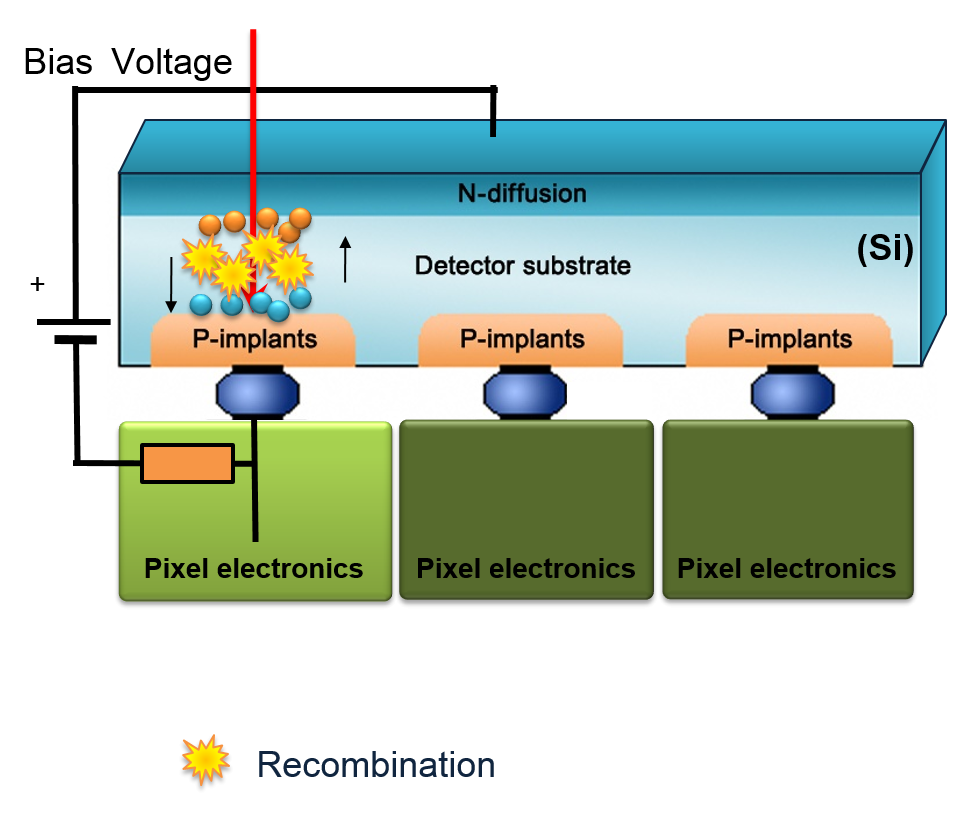
\includegraphics[width=8.5cm]{figures/det_recombination.png}
		\caption{Princip detekce ionizujícího záření (převzato z \cite{PlatkevicDisertace})}
		\label{fig:det:recomb}
	\end{center}
\end{figure}

%********************************************************************************
% Princip detekce
%********************************************************************************
\section{Princip detekce}
Činnost těchto detektorů je založena na známém principu detekce ionizujícího záření v polovodiči. 

Na obrázku \ref{fig:det:recomb} je znázorněn princip této detekce. V horní části se nachází polovodičový senzor, pro který je jako materiál nejčastěji použit křemík, ale výjimkou není také \texttt{GaAs}, či \texttt{CdTe}. Pod tímto senzorem se nachází vyčítací elektronika, která tvoří jednotlivé pixely. Jako náhradní schéma tohoto obvodu si můžeme představit diodu zapojenou v závěrném směru, skrze kterou protéká jen minimální proud. Vnikne-li ale do polovodičového senzoru ionizovaná částice, která v senzoru zanechá jisté množství své deponované energie, dojde ke vzniku elektron-děrových párů a díky lavinovému jevu i k následnému otevření PN přechodu. Tím dojde k vyvolání proudového pulsu, které je pomocí měřícího odporu převeden na napětí, které je dále měřící elektronikou zpracováváno.

\begin{figure}[th]
	\begin{center}
		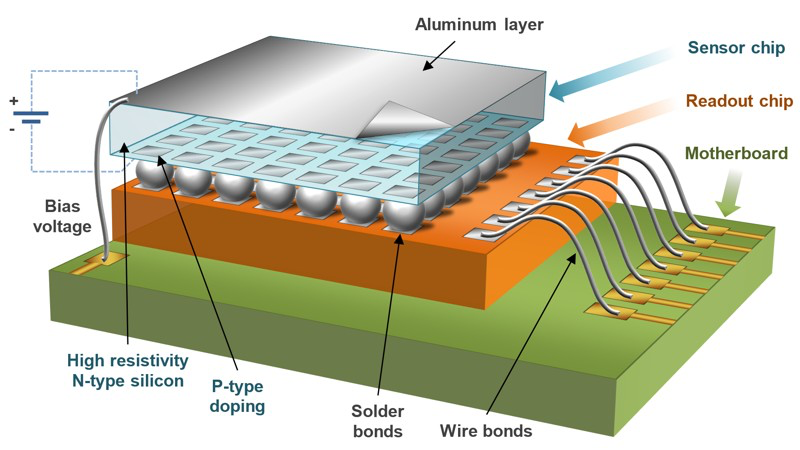
\includegraphics[width=12cm]{figures/det_chip.png}
		\caption{Struktura hybridního polovodičového pixelového detektoru (převzato z \cite{PlatkevicDisertace})}
		\label{fig:det:chip}
	\end{center}
\end{figure}

Na obrázku \ref{fig:det:chip} je znázorněna struktura tohoto detektoru. Nahoře se nachází, již výše zmíněný, polovodičový senzor, který je spojen s integrovaným \texttt{ASIC}\footnote{z angl. Application Specific Integrated Circuit} vyčítacím čipem (tzv. \texttt{Readout chip}) pomocí technologie zvané \texttt{bump-bonding}. Odtud také pochází název "hybridní" - jedná se spojení senzoru a \texttt{ASIC} čipu. Každý pixel tedy tvoří jeden PN přechod. Vyčítací čip je dále spojen s další nezbytnou elektronikou (na obr \ref{fig:det:chip} znázorněnou jako \texttt{Motherboard}) pomocí tzv. \texttt{wire-bonds}. Z této elektroniky je dále vyvedeno napětí na polovodičový senzor - \texttt{bias}.

%********************************************************************************
% Medipix detektory
%********************************************************************************
\section{Detektory rodiny Medipix}\label{det:med}
Mezi mezi nejznámější detektory rodiny Medipix patří: Medipix1, Medipix2 \cite{Llopart-medipix2}, Timepix \cite{Llopart2008106}, Medipix3, nově Timepix3 \cite{timepix3} a v průběhu příštího roku k nim přibude i Timepix2. 

\begin{description}
	\item[Medipix1] Medipix1 byl prvním detektorem z této rodiny a byl uvedený v roce 1997. Také je známy pod názvem PCC (z angl. Photon Counting Chip). Jednalo se o prototyp digitálního \texttt{CMOS}\footnote{z angl. Complementary Metal–Oxide–Semiconductor} zobrazovacího čipu, který našel uplatnění ve vysokoenergetických fyzikálních experimentech \cite{medipix-www} a byl schopný operovat jen v \texttt{Medipix módu} (viz \ref{det:mod}). Tento detektor měl matici $64\times64$ pixelů, každý s hranou o délce $170~\mu m$ a celková aktivní plocha byla $1,2~cm^2$. Detektor obsahoval $15$-bitový čítač, kterým byl schopen v rámci jedné akvizice zaregistrovat až $32767$ událostí.

	\item[Medipix2] Medipix2 je přímým následníkem Medipix1. Tento model především profitoval z rychlého pokroku \texttt{CMOS} technologie, díky kterému bylo možné přidání nové funkcionality a především zmenšení velikosti pixelů. Detektor obsahoval matici $256\times256$ pixelů, délka hrany jednoho pixelu se zmenšila na $55~\mu m$ a celková aktivní plocha vzrostla na $2~cm^2$.

	\item[Timepix]\label{det:tim} Tento detektor vychází z detektoru Medipix2, prodělal však výraznou obměnu digitální části. Byla přidána synchronizační logika, která přinesla dva nové módy - TOT (měření energie) a TOA (měření doby příletu částice), přičemž každý pixel v jeden okamžik umožňuje měřit jen v jednom módu
	(vice o módech bude zmíněno v \ref{det:mod}). Další možností je nastavení globálního tresholdu\footnote{Treshold je úroveň komparačního napětí, které je porovnáváno s aktuálním měřícím napětím na každém pixelu. Je-li tato úroveň překročena, dojde k detekováni události.} s lokální úpravou pro jednotlivé pixely o $4 b$. 

	\item[Medipix3] U Medipix3, jehož předchůdce byl Medipix2, byla výrazným způsobem přepracována vyčítací elektronika za cílem snížení zkreslení, způsobeném sdílením náboje mezi sousedními pixely (tento efent je také znám pod pojmem \texttt{Charge Sharing} efekt \cite{Jakubek-radiography_and_charge_sharing}). 

	\begin{figure}[th]
	\begin{center}
		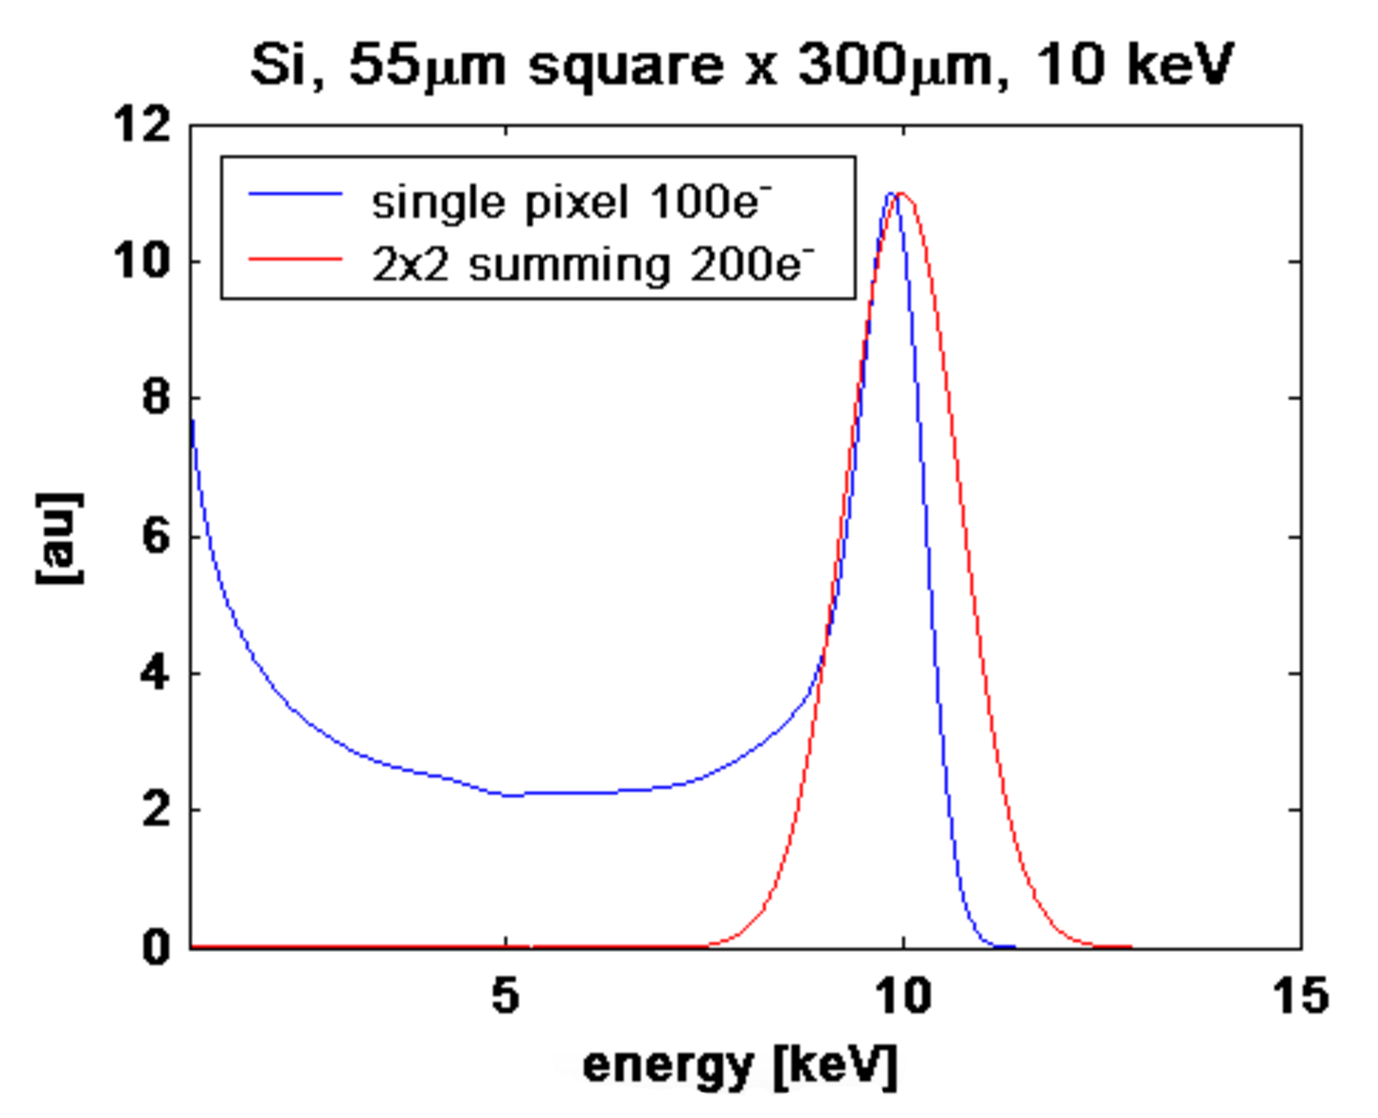
\includegraphics[width=8cm]{figures/det_charge_sharing.png}
		\caption{Charge Sharing Efekt (převzato z \cite{medipix-www})}
		\label{fig:det:charge_sharing}
	\end{center}
	\end{figure}

	Když dopadne nabitá částice na polovodičový senzor, vzniknou elektron-děrové páry, které jsou staženy nejen zasaženým pixelem, ale vetšinou i několika sousedními. To samo o sobě je žádoucí jev, problém ale nastává, když vyčtená energie sousedními pixely je nižší, než jejich prahová, potom dochází ke, již výše zmíněnému, zkreslení. 
	
	Obrázek \ref{fig:det:charge_sharing} je demonstrací tohoto jevu. Zobrazuje histogram detekovaných energií pro jeden pixel. Když každý pixel operuje zcela nezávisle (na obrázku modře), je patrné, že daný pixel registroval i události sousedních pixelů, vzniklé \texttt{Charge Sharing} efektem. Tento problém odstraňuje \texttt{CSM} \ref{det:mod:csm} mód a především možnost vyčítat jednotlivé události (nikoliv až celé snímky), což také odstraňuje mrtvou dobu detektoru. \texttt{CSM} mód přičte k energii zasaženého pixelu i energii sousedních pixelů - viz obr. \ref{fig:det:charge_sharing} červeně.

	\item[Timepix3] Nejnovějším přírůstkem této rodiny detektorů je Timepix3. Oproti svému předchůdci Timepix má tento detektor vylepšenou vyčítací logiku a o jeden čítač více. To mu mimo jiné umožňuje měřit v TOT a TOA módu současně. Navíc ještě přináší \texttt{Data-driven} vyčítací mód (obdobně, jako Medipix3), který na rozdíl od \texttt{Frame-based} vyčítání odstraňuje mrtvou dobu detektoru.

\end{description}

%********************************************************************************
% Módy detektorů
%********************************************************************************
\section{Módy detektorů}\label{det:mod}
V této podkapitole budou popsány všechny nejpoužívanější módy detektorů z rodiny Medipix. 
Na obrázku \ref{fig:det:signal_proc} jsou znázorněny tři pixely detektoru s blokovým schématem vyčítací elektroniky. Jak již bylo zmíněno výše, interagující částice s polovodičovým povrchem detektoru vyvolá proudový pulz. Ten je měřícím odporem převeden na napětí, které je dále zesilovačem zesíleno (na obr. \ref{fig:det:signal_proc} jako \texttt{Amplifier}). Toto napětí je dále porovnáno komparátorem s komparačním napětím (tzv. tresholdem), jak je znázorněno na obr. \ref{fig:det:signal_proc}. S informací z tohoto komparátoru je dále naloženo dle módu detektoru. Pro úplnost je třeba dodat, že \texttt{Shutter} na obr. \ref{fig:det:signal_proc} slouží pro spouštění, resp. ukončování akvizice.

\begin{figure}[th!]
	\begin{center}
		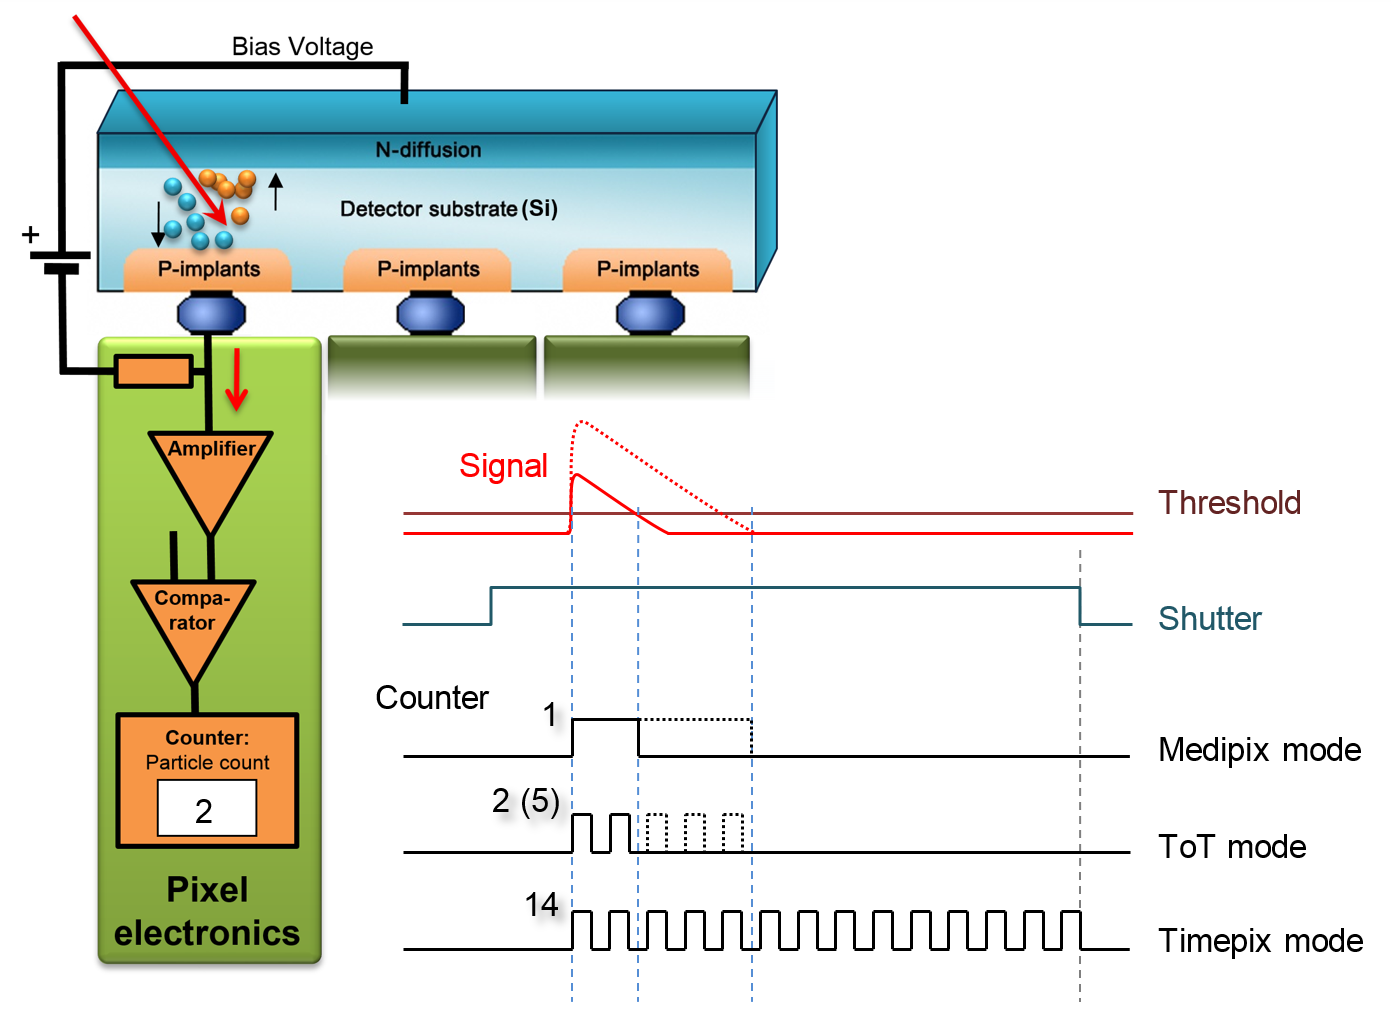
\includegraphics[width=10.75cm]{figures/det_pix.png}
		\caption{Zpracování signálu z pohledu módu pixelu (převzato z \cite{PlatkevicDisertace})}
		\label{fig:det:signal_proc}
	\end{center}
\end{figure}

\begin{description}
	\item[Medipix mód] Tento mód počítá počet částic, které během doby akvizice dopadly na aktivní plochu detektoru. Na obrázku \ref{fig:det:signal_proc} znázorněn, jako \texttt{Medipix mode}.
	\item[TOT (Time-Over-Treshold)] Tento mód udává, jak dlouhou dobu (v počtu hodinových cyklů měřící frekvence) bylo zesílené napětí na detektoru vyšší, než komparační (treshold). Počet těchto cyklů je zhruba ekvivalentní energii deponované částice, ale jelikož každý pixel má jiné elektronické vlastnosti, je třeba pro získání energie z TOT detektor kalibrovat - o tom pojednává kapitola \ref{calib}. Tento mód je podporovaný všemi Timepix detektory (ze zde uvedených detektorů).
	\item[TOA (Time-Of-Arrival)] Pixel v tomto módu spustí svůj čítač po překročení tresholdu, čily vůči akvizičnímu času udává čas příletu částice. Tento mód je také známý pod označením \texttt{Timepix mode} a nalézá své uplatnění především při měření koincidencí (rekonstrukce trajektorie částice, interagující s více detektory pomocí času dopadu a souřadnic zasažených pixelů). Tento mód je podporovaný všemi Timepix detektory (ze zde uvedených detektorů).
	\item[SPM (Single Pixel Mode)] V tomto módu každý pixel operuje zcela samostatně a to v Medipix módu.
	\item[CSM (Charge Summing Mode)]\label{det:mod:csm} Tento mód odstraňuje zkreslení vzniklé \texttt{Charge Sharing} efektem pomocí přičtení energie do zasaženého pixelu z pixelů okolních. Jako zasažený pixel se určí pixel s nejvyšší energií. Tento mód podporuje jen Medipix3 (ze zde uvedených detektorů).

\end{description}

%********************************************************************************
% FITPix
%********************************************************************************
\section{FITPix}\label{det:fitpix}

\begin{figure}[th!]
	\begin{center}
		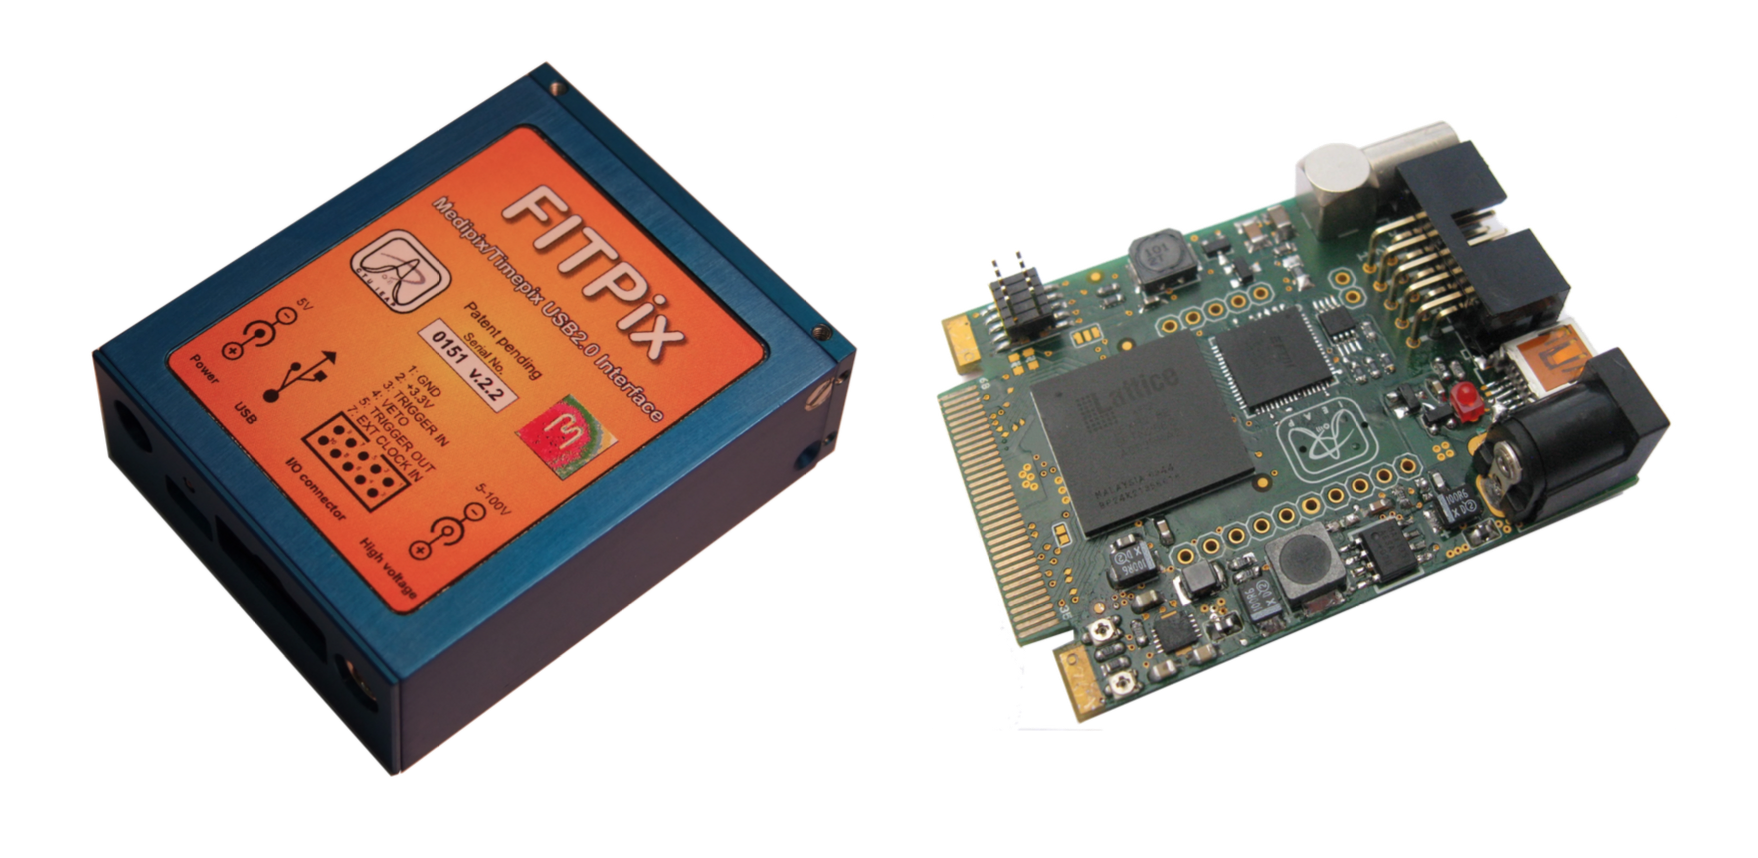
\includegraphics[width=11cm]{figures/fitpix.png}
		\caption{FITPix}
		\label{fig:det:fitpix}
	\end{center}
\end{figure}

FITPix\footnote{z angl. Fast Interface for Timepix Pixel Detectors} \cite{fitpix} je vyčítací rozhraní, pracující téměř se všemi detektory rodiny Medipix, vyvíjené v ÚTEF ČVUT v Praze od roku 2010 - viz obr. \ref{fig:det:fitpix}. Toto rozhraní se skládá z FPGA\footnote{z angl. Feld Programmable Gate Array} obvodu, USB 2.0 rozhraní, DAC převodníků (převodník digitálního signálu na analogový), ADC převodníků (převodník analogového signálu na digitální) a z obvodů generující napětí pro polovodičový senzor (tzv. bias). Toto zařízení umožňuje plnohodnotné ovládání připojeného detekčního čipu, včetně nastavování měřící frekvence, tresholdu, řízení shutteru (sloužícího pro ovládání akvizice, viz \ref{det:mod}) apod. Také přináší možnost ovládat shutter pomocí hardwarového trigger signálu pro měření s více detektory současně, resp. pro jejich synchronizaci.

Tato architektura s FPGA byla použita především z důvodu dosažení vyšších datových toků a také vyšší radiační odolnosti, které by za použití konvenčních mikroprocesorů nemohlo být dosaženo. Další výhodou je menší počet aktivních prvků, což se projeví krom spotřeby i na nižších tepelných ztrátách. Tento parametr je velice důležitý, především pro nasazení ve vakuu.

%********************************************************************************
% Pixelman
%********************************************************************************
\section{Pixelman}\label{det:pixelman}
Pixelman \cite{pixelman} je softwarový balík, vyvíjený v ÚTEF ČVUT v Praze, sloužící pro řízení detektorů z rodiny Medipix pomocí vyčítacího rozhraní FITPix \ref{det:fitpix}. Tento software umožňuje akvizici dat, jejich vizualizaci a následnou analýzu.

Jedná se o vysoce modulární systém, který mimo jiné umožňuje rozšíření své funkcionality o pluginy, které mají přístup k funkcím, poskytovaným jádrem Pixelmanu. Dokonce každý plugin může zaregistrovat své funkce, takže i ostatní pluiny mohou využívat jeho funkcionalitu. Jsou podporovány pluginy, vyvinuté v jazycích Java, C/C++ a Python. Na obrázku \ref{fig:det:pixelman} je znázorněna softwarová architektura Pixelmana.

\begin{figure}[th!]
	\begin{center}
		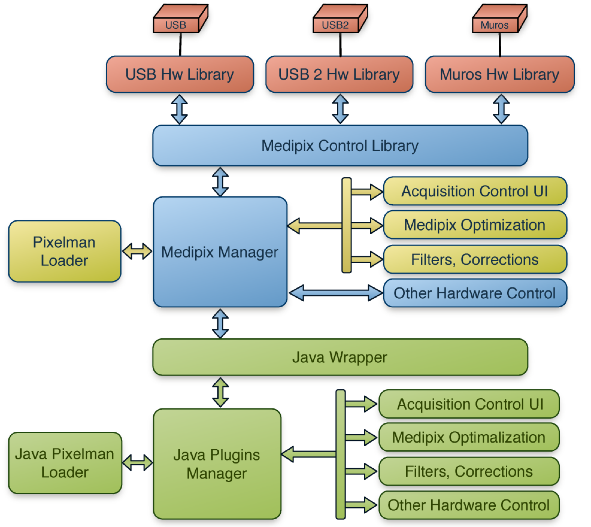
\includegraphics[width=10.25cm]{figures/pixelman.png}
		\caption{Pixelman - sw architektura (převzato z \cite{pixelman})}
		\label{fig:det:pixelman}
	\end{center}
\end{figure}


%********************************************************************************
% Aplikace
%********************************************************************************
%\section{Aplikace}









\addbibresource{reference.bib}

\chapter{Energetická kalibrace}\label{calib}
Tato kapitola pojednává o metodách energetické kalibraci hybridních částicových pixelových detektorů, pracujících v~Time-Over-Treshold módu a~o implementaci jedné z~nich pro účely kalibrace detektorů sítě ATLAS TPX.

%********************************************************************************
% Motivace
%********************************************************************************
\section{Motivace}
%Hybridní částicové pixelové detektory typu Timepix (viz \ref{det:tim}), disponují módem TOT (Time-Over-Treshold), který lze využít pro měření energie ionigujícího záření dopadajícího na aktivní plochu detektoru. Když s pixel pracuje v~tomto módu a~intaraguje s~ním částice, dojde k~vygenerování napěťového pulzu, jehož velikost je úměrná deponované energii interagující částice (viz kapitola \ref{det:mod}). Je-li velikost tohoto pulzu větší, než treshold zasaženého pixelu, tak dojde ke spuštění čítače, který začne počítat hodinové cykly měřící frekvence a~zastaví se tehdy, když klesne hodnota napětí na původní hodnotu, pod úroveň tresholdu. Po skončení akvizice je hodnota tohoto čítače rovna hodnotě TOT, která odpovídá deponované energii interagující částice. Vztah mezi TOT a~energií je ale nelineární a~je podmíněn různými elektronickými a~fyzikálními vlastnostmi daného pixelu. Určení tohoto vztahu je předmětem kalibrace, o které tato kapitola bude pojednávat.

Každý detektor ionizujícího záření je třeba pře použitím zkalibrovat pomocí známých zrojů záření. Vzniká tak přepočet vnitřních elektrických veličin detektoru na energii. Pro účely fyzikálních měření je zvykem užívat jako jednotku energie eV, resp. keV. 
V případě detektoru Timepix se z důvodu nelineární odezvy (obr. \ref{fig:calib:calib_function}) pixelové elektroniky jedná o~netriviální úlohu. Cílem kalibrace je nalézt parametry analyticky popisující kalibrační křivku, na příklad pomocí funkce \ref{eq:calib:calib_function}.

\begin{figure}[th!]
	\begin{center}
		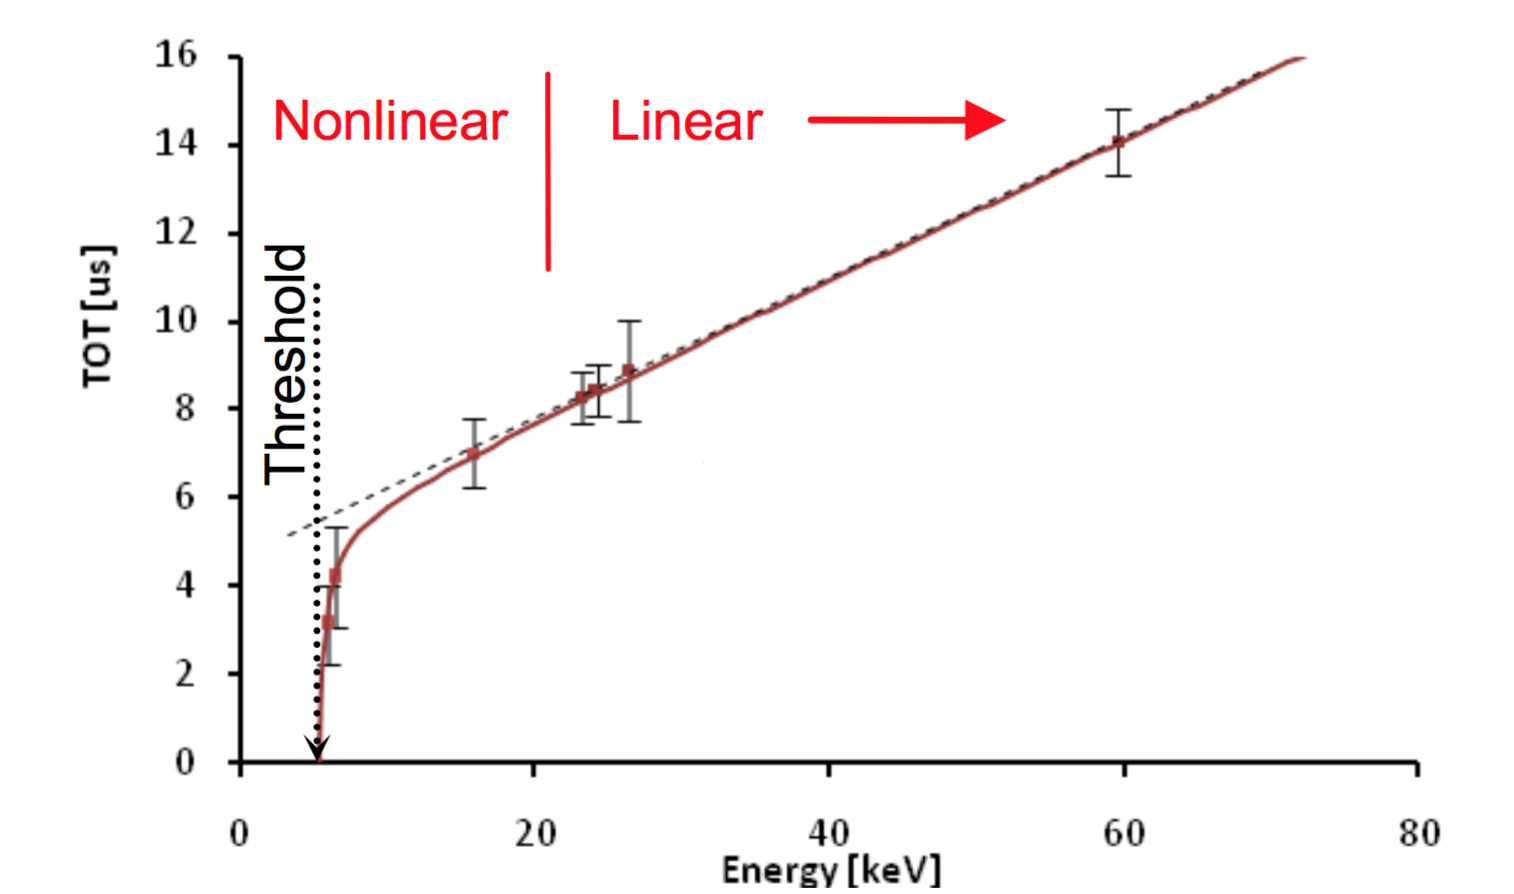
\includegraphics[width=8cm]{figures/calib_function.png}
		\caption{Kalibrační funkce (převzato z~\cite{Jakubek2011S262}) udává závislost mezi energií a TOT. Vzniká proložením naměřených kalibračních bodů pomocí funkce \ref{eq:calib:calib_function}. Tato funkce vznikla složením hyperboly (popisující nelineární oblast nižších energií) a~přímky (pro oblast s vyšší energií).}
		\label{fig:calib:calib_function}
	\end{center}
\end{figure}


\begin{equation}\label{eq:calib:calib_function}
	f_{calib}(x) = ax + b - \frac{c}{x-t}
\end{equation}

%\newpage

%********************************************************************************
% Přehled kalibračních metod
%********************************************************************************
\section{Přehled kalibračních metod}

%********************************************************************************
% Přehled kalibračních metod
% > X-ray
%********************************************************************************
\subsection{Kalibrace detektorů za použití rentgenového záření}\label{calib:xray}
Tato kalibrační metoda \cite{Jakubek2011S262} spočívá v~měření rentgenové fluorescence (viz \cite{Jakubek-radiography_and_charge_sharing}),
což je děj, ke kterému dochází, když je materiál\footnote{Pro kalibraci se používají kovy, na příklad Am, In, Cu, Fe apod.} (terč)
ozařován rentgenovým zářením, které vyráží excitované elektrony z~jeho atomů. Je-li vyražen elektron na nižší energetické úrovní, tak elektron z~vyšší energetické úrovně deexcituje a~obsadí jeho místo. 
Přebytečnou energii ztratí ve formě vyzářeného fotonu (tzv. charakteristické záření). Spojitou část rentgenového spektra je potřeba odstínit. Výběrem vhodných terčů lze získat několik diskrétních energií záření, tzv. kalibrační body. Z důvodů statistických vlastností záření je třeba pro každý kalibrační bod pořídit velké množství snímků, ze kterých jsou následně vyfiltrovány jen tzv. \texttt{Single-Hit} události,
%Díky této fluorescenci je detektor pomocí různých mono-energetických zdrojů záření, jejichž energie je předem známa, postupně ozařován. V~rámci tohoto měření je třeba pro každý zdroj pořídit velké množství snímků, ze kterých jsou následně vyfiltrovány jen tzv. \texttt{Single-Hit}
při kterých interagující částice zasáhla jen jeden pixel. 
Tyto události jsou filtrovány, z důvodu dosažení vyšší kvality kalibrace, pomocí potlačení zkreslení způsobeného \texttt{Charge Sharing} efektem\footnote{Když dopadne nabitá částice na polovodičový senzor, vzniknou elektron-děrové páry, které jsou staženy nejen zasaženým pixelem, ale vetšinou i několika sousedními. To je dáno jednou společnou elektrodou pro všechny pixely senzoru (viz obr. \ref{fig:det:chip}).}.

\begin{figure}[th]
	\begin{center}
		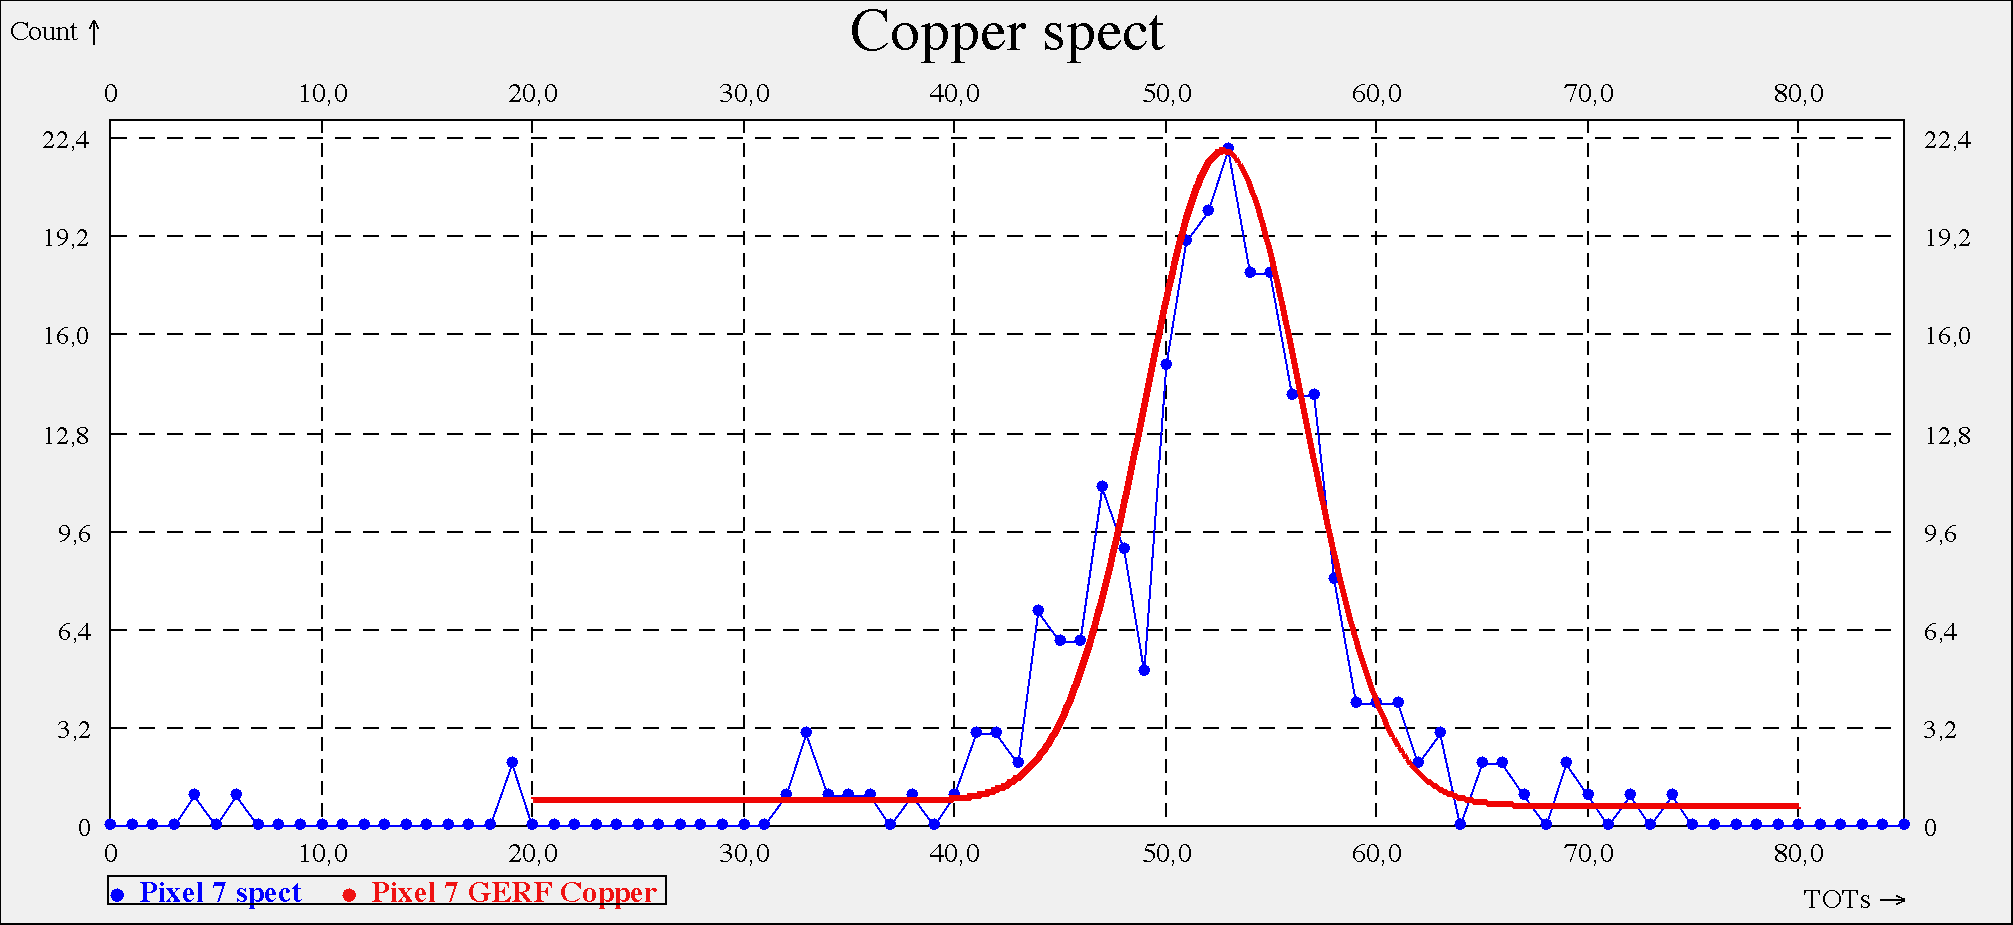
\includegraphics[width=14cm]{figures/calib_gerf.png}
		\caption{Spektrum TOT hodnot jednoho pixelu s~proložením Gaussovou funkcí, sečtenou s~Gaussovou chybovou funkcí (tzv. error funkce). Zdrojem rentgenové fluorescence byla měď.}
		\label{fig:calib:gerf}
	\end{center}
\end{figure}

%Dalším krokem tohoto procesu je získání jednotlivých kalibračních bodů, udávajících závislost mezi jednotlivými energiemi a~TOT hodnotami. Toho je možné docílit vytvořením spekter pro jednotlivé pixely a~zdroje záření.
Na obrázku \ref{fig:calib:gerf} je příklad spektra pro jeden pixel detektoru a~fluorescenčního záření z~mědi. Na vodorovné ose tohoto spektra se nachází jednotlivé TOT hodnoty a~na svislé pak jejich četnost ve všech snímcích. Z~obrázku je patrné, že nejčetnější hodnotou TOT je zhruba hodnota $53$, která odpovídá energii fluorescenčního záření mědi, což je $5,9~keV$. Požadovanou hodnotu TOT lze získat proložením spektra funkcí \ref{eq:calib:gerf}. Ta vznikla z~Gaussovy funkce, ke které byla z~důvodu levé nesymetrie, způsobené \texttt{Charge Sahring} efektem, přičtena Gaussova chybová funkce. 

\begin{equation}\label{eq:calib:gerf}
	f_{GERF}(x) = \underbrace{Ae^{ -\frac{(x-\mu)^2}{2\sigma^2} }}_{\text{Gaussova funkce}} +
	\underbrace{ \frac{avg_{right} - avg_{left}}{\sigma\sqrt{2\pi}} \int_{-\infty}^t e^{ -\frac{(t-\mu)^2}{2\sigma^2} } + avg_{left}}_{\text{Gaussova chybová funkce}}
\end{equation}

Parametry funkce \ref{eq:calib:gerf} jsou následující:
\begin{itemize}
	\item $\mathbf{A}$ je amplituda.
	\item $\mathbf{\mu}$ je stření hodnota hledané energie.
	\item $\mathbf{\sigma}$ udává rozptyl střední hodnoty energie $\mu$, kterou je možné ji vypočítat ze vzorce 
		$\sigma = \frac{2\sqrt{2ln_2}}{FWHM}$, kde $FWHM$\footnote{z angl. Full Width at Half Maximum} udává šířku gausiánu v~polovině jeho výšky.
	\item $\mathbf{avg_{right}}$ (resp. $\mathbf{avg_{left}}$) je průměrná hodnota spektra na pravém (resp. levém) úpatí gausiánu.
\end{itemize}

Z těchto kalibračních bodů je možné sestavit kalibrační funkci (viz vzorec \ref{eq:calib:calib_function}), udávající závislost mezi energií a~TOT.


%********************************************************************************
% Přehled kalibračních metod
% > LED
%********************************************************************************
\subsection{Kalibrace detektorů pomocí LED diod}\label{calib:led}
Princip kalibrace pomocí SMD LED diod spočívá v~působení přesného množství světelného záření na polovodičový senzor detektoru. V~současné době je tato metoda ve fázi vývoje a~doposud nebyla publikována. Metoda je použitelná pouze pro detektory, na jejichž senzoru není napařena tenká vrstva hliníku, která světelné záření nepropouští. 

Jako zdroj světla byl v~ÚTEF vyvinut modul s~maticí $8\times8$ SMD LED diod, který je možné ovládat pomocí \texttt{RS232} sériové linky. K~tomuto modulu byl rovněž vytvořen plugin do softwarového balíku Pixelman \ref{det:pixelman}, který automatizuje proces nabírání dat této metody. Přes sériovou linku je schopen řídit modul s~LED diodami a~zároveň pomocí jádra Pixelmanu ovládá akvizici dat detektoru.

Kroky algoritmu kalibrace jsou následující:
\begin{enumerate}
	\item Inicializace:
		\begin{itemize}
			\item nastavení spouštění akvizice detektoru na externí hardwarový trigger (který bude ovládán modulem s~LED diodami)
			\item nastavení energie světelného záření (počet zabliknutí diody, délka periody jednoho bliknutí a~doba aktivace diody v~jedné periodě)
			\item  délku akvizice snímku (vypočtené dle periody blikání a~počet opakování)
		\end{itemize}
	\item Měřící smyčka (opakuje se pro všechny LED diody). V~rámci jednoho průchodu se provede následující:
		\begin{itemize}
			\item Zamaskování všech pixelů detektoru, krom těch pixelů, které jsou pod aktivní diodou.
			\item Spuštění akvizice.
			\item Vyčtení a~uložení snímku z~detektoru.
		\end{itemize}
	\item Následně se hodnoty všech snímků sečtou do jednoho snímku - viz obr. \ref{fig:calib:led_frame}.
\end{enumerate}

\begin{figure}[th]
	\begin{center}
		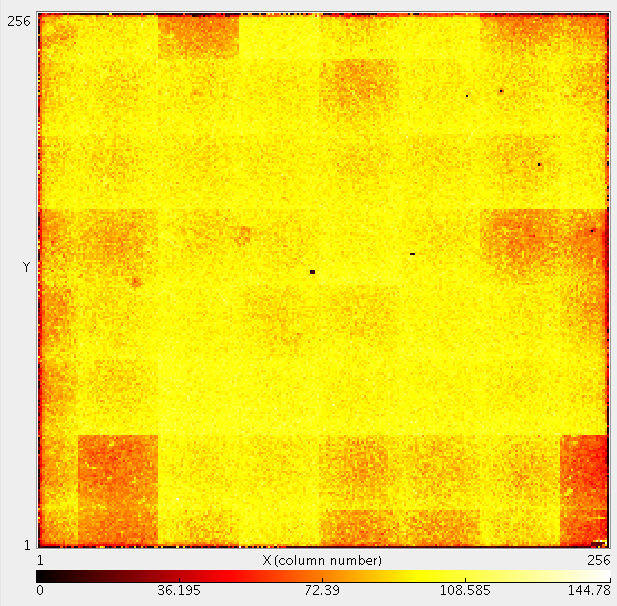
\includegraphics[width=10cm]{figures/led_calib_frame.png}
		\caption{Snímek z~detektoru, ozařovaném modulem s~LED diodami}
		\label{fig:calib:led_frame}
	\end{center}
\end{figure}

Z obrázku \ref{fig:calib:led_frame} jsou patrné hrany jednotlivých dílčích měření, které vznikly nehomogenitou elektronických vlastností jednotlivých diod. Tento jev může být odstraněn normalizací jejich světelné intenzity pomocí vynásobení času aktivace každé diody normalizační maticí.
% jejich kalibrací, jejíž výstupem bude normalizační matice, kterou se vynásobí čas aktivace každé diody, což bude předmětem dalšího výzkumu této metody.

Tímto způsobem jsou pro každý pixel detektoru získají jednotlivé kalibrační body, které jsou následně proloží kalibrační funkcí (viz vzorec \ref{eq:calib:calib_function}), jak již bylo popsáno v~kapitole \ref{calib:xray}.


\newpage
%********************************************************************************
% X-ray Calib impl
%********************************************************************************
\section{Software pro kalibraci detektorů za použití rentgenového záření}\label{calib:sw}

Tato podkapitola pojednává o softwaru pro energetickou kalibraci pixelových detektorů za použití kalibrační metody s~rentgenovým zářením (viz \ref{calib:xray}). Tento software původně vznikal pro účely kalibrace sítě ATLAS TPX, avšak později byl rozšířen a~nyní je kompatibilní se všemi detektory, pracujícími v~TOT módu. Software vyl vyvinut v~programovacím jazyce \texttt{Java} a~grafické rozhraní bylo vytvořeno za pomoci knihovny \texttt{Swing}. V~rámci této práce rovněž vznikla vlastní knihovna pro vizualizaci 2D grafů.

Jak již bylo zmíněno v~kapitole \ref{calib:xray}, proces kalibrace se skládá z~několika kroků, a~to z~vytvoření spekter pro jednotlivé pixely a~zdroje záření, následném nalezení kalibračních bodů z~těchto spekter a~vytvoření kalibrační funkce pro každý pixel detektoru. Na obrázku \ref{fig:calib:sw_process_ops} je znázorněna možnost nastavení provedení jednotlivých kroků kalibračního procesu nad zvolenými měřeními (viz obr. \ref{fig:calib:sw_spektra} - levý postranní panel), v~rámci jednoho průchodu po stisknutí tlačítka \texttt{Start/Abort} (viz obr. \ref{fig:calib:sw_spektra} vlevo dole).

\begin{figure}[th]
	\begin{center}
		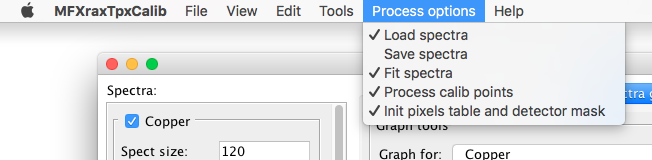
\includegraphics[width=14cm]{figures/calibsw_process_ops.png}
		\caption{Screenshot kalibračního softwaru - volby zpracování v~rámci kalibračního procesu}
		\label{fig:calib:sw_process_ops}
	\end{center}
\end{figure}


%********************************************************************************
% X-ray Calib impl
% > Vstupní data kalibrace
%********************************************************************************
\subsection{Vstupní data kalibrace}
Vstupní data se skládají z~několika sad měření pro různé zdroje mono-energetického ionizujícího záření (např. fluorescenčního), jejichž energie jsou předem známy. Z~naměřených hodnot jsou vytvořena spektra pro každý pixel detektoru (příkladem takového spektra může být obrázek \ref{fig:calib:sw_spektra}.%, na kterém je screenshot kalibračního softwaru se spektrem jednoho pixelu pro měření gama emise americia a~fluorescence india).

\begin{figure}[t]
	\begin{center}
		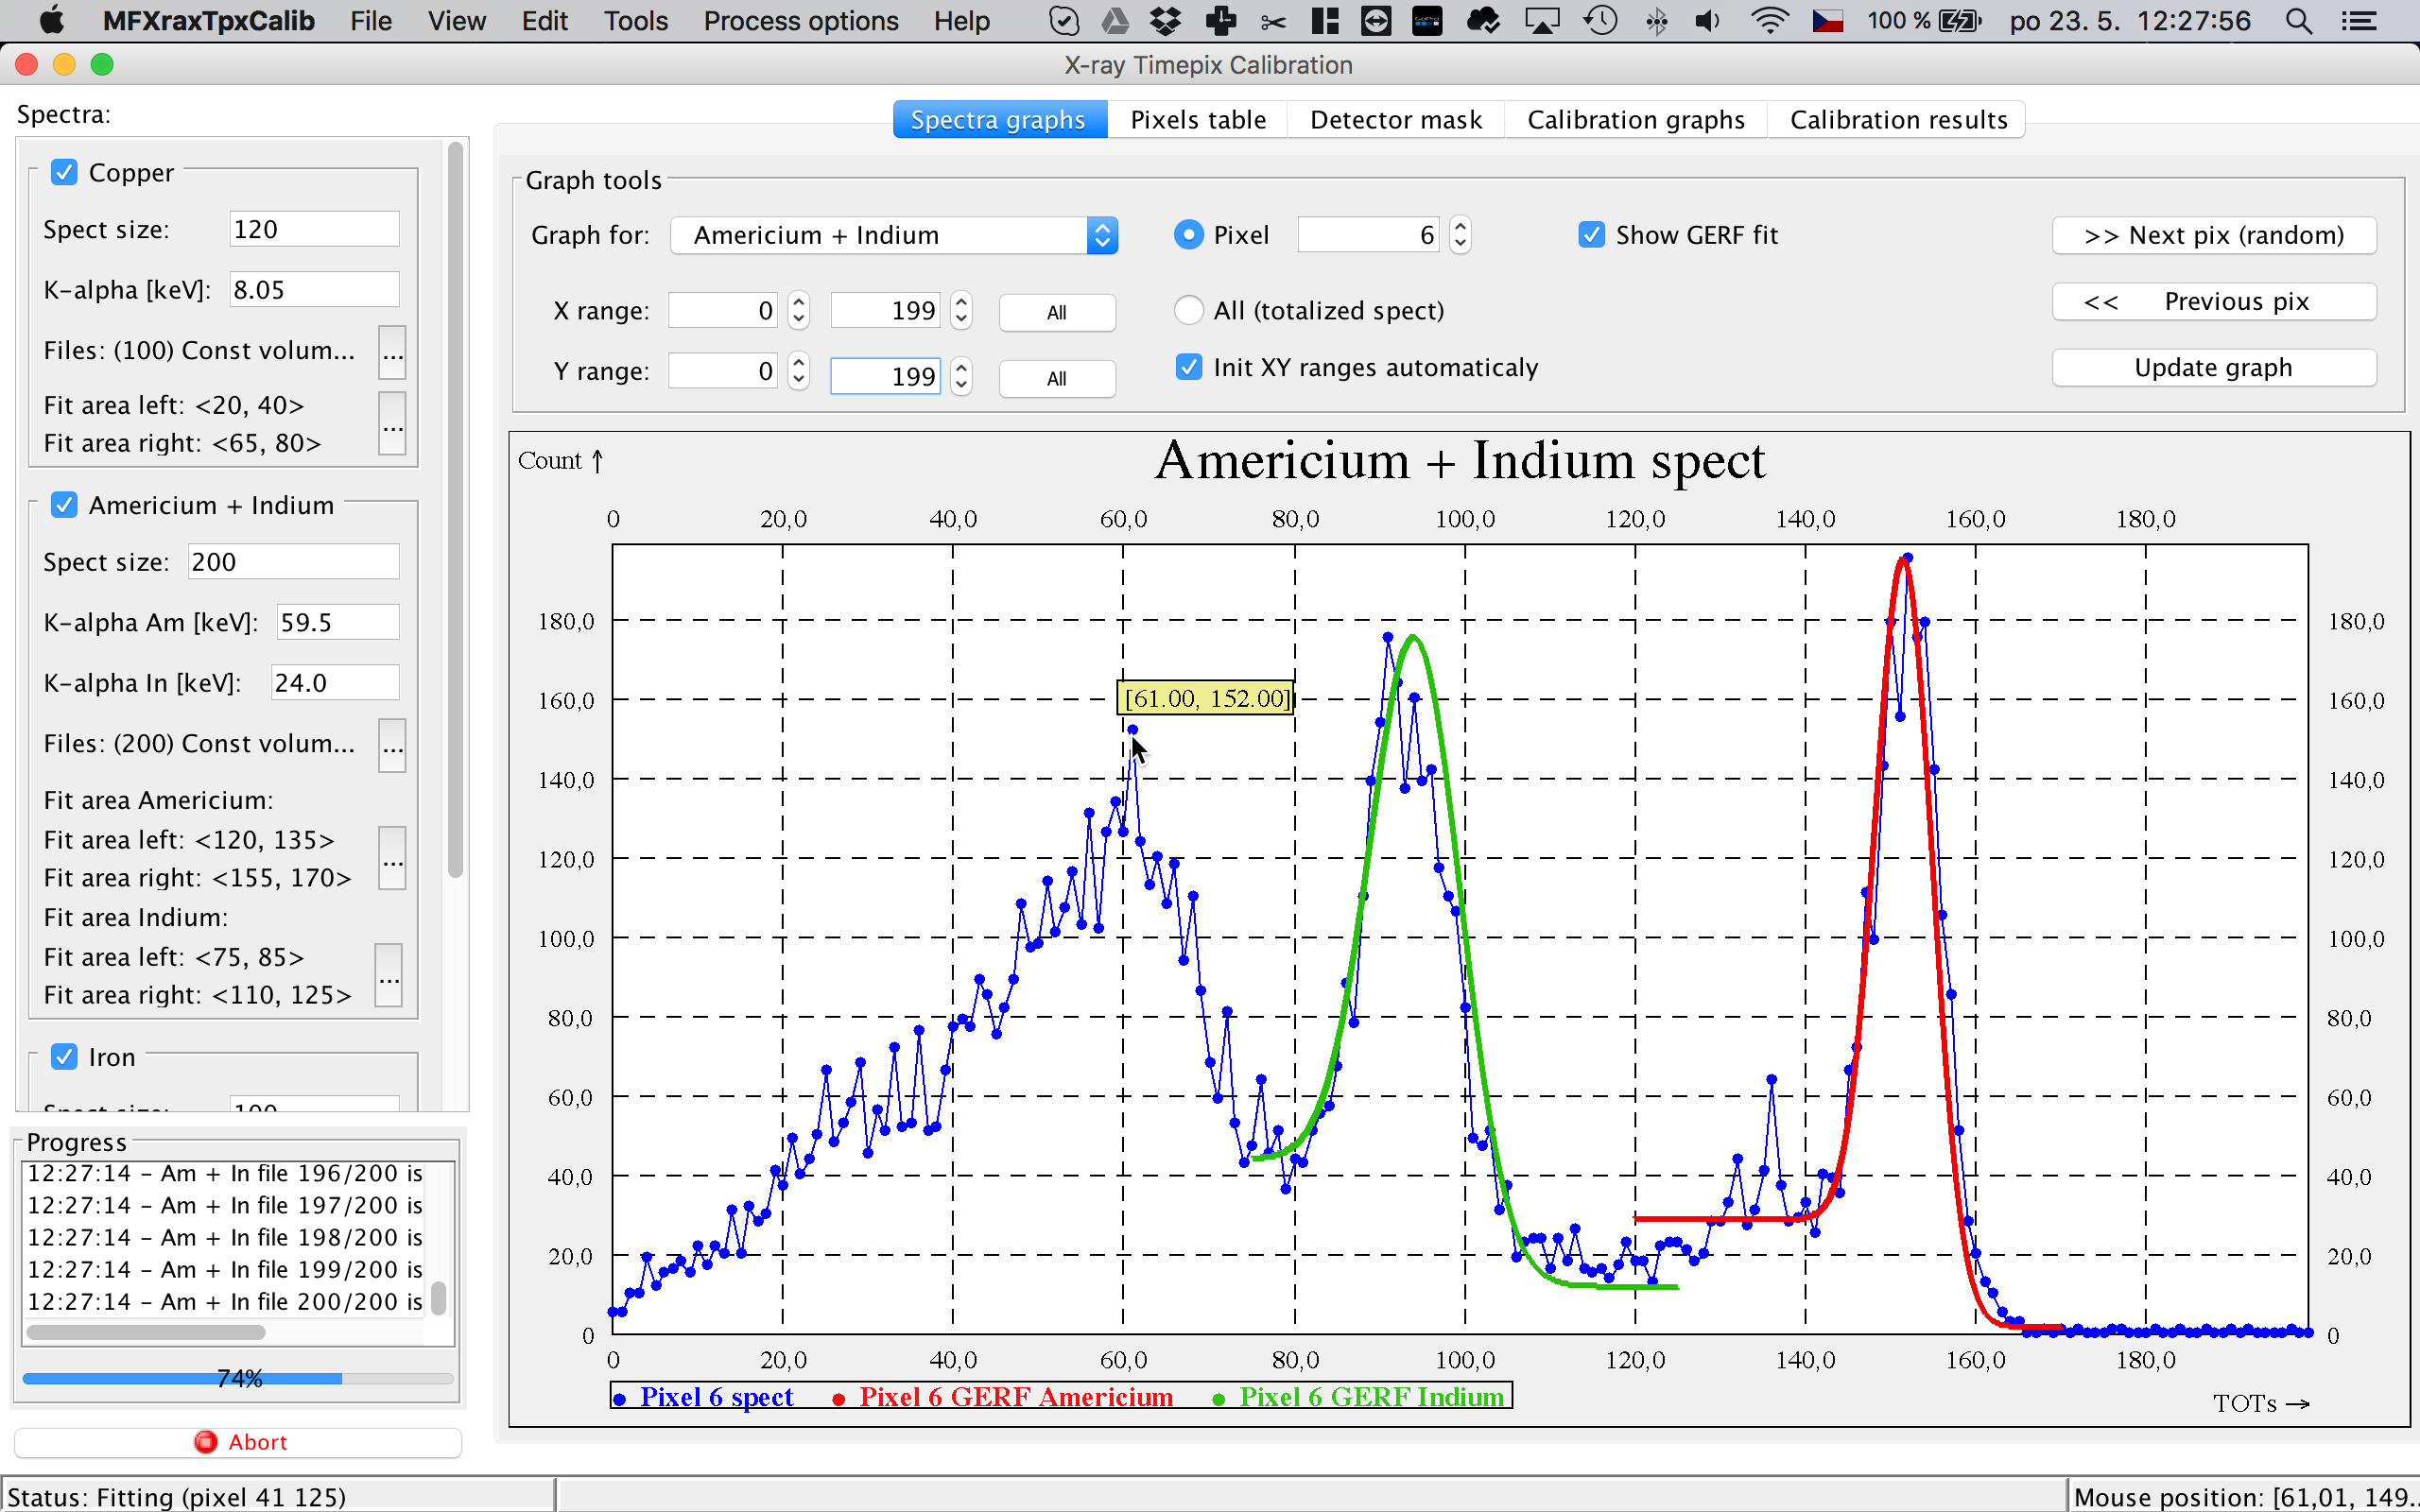
\includegraphics[width=15cm]{figures/calibsw_spectra_all.png}
		\caption{Screenshot kalibračního softwaru, zobrazující složené spektrum pro gama emisi americia (pravý červený pík) a~fluoresceni india (levý zelený pík), proložené funkcí \ref{eq:calib:gerf}. Levou část spekta tvoří fotony vzniklé Comptonovým rozptylem.}
		\label{fig:calib:sw_spektra}
	\end{center}
\end{figure}

K výběru vstupních dat slouží postranní panel hlavního okna kalibračního softwaru, kde je seznam jednotlivých měření. K~manipulaci s~položkami v~tomto seznamu slouží \texttt{Measurement manager} (dostupný ze záložky \texttt{File} v~hlavní liště - viz obr. \ref{fig:calib:sw_measurmanag}). V~rámci tohoto nástroje je možné přidávat, odebírat, či jinak upravovat jednotlivá měření a~jejich parametry (například velikost spektra apod.). Každé měření může obsahovat až tři kalibrační body, jejichž parametry je možné také nastavit skrze \texttt{Measurement manager}.

\begin{figure}[th!]
	\begin{center}
		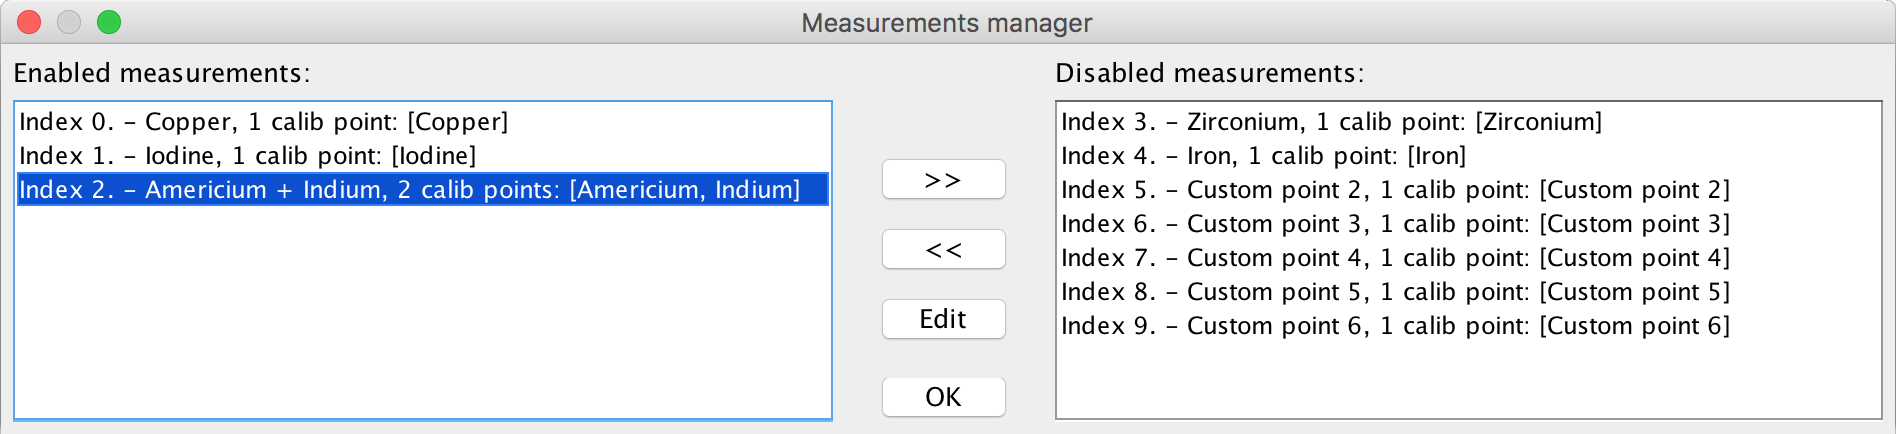
\includegraphics[width=15cm]{figures/calibsw_manager.png}
		\caption{Screenshot kalibračního softwaru - Measurement manager}
		\label{fig:calib:sw_measurmanag}
	\end{center}
\end{figure}

Vstupní data jsou podporována ve třech formátech:
\begin{description}
	\item[Multiframe] Formát slouží pro hromadné ukládání surových snímků z~detektoru, kde jsou jednotlivé snímky zapsány jako seznam zasažených pixelů a~jejich hodnot (pro více o tomto formátu viz \ref{atlas:cont:output}). Každý snímek je třeba načíst a vyfiltrovat pouze \texttt{Single-Hit} události (viz \ref{calib:xray}), ze kterých jsou následně vytvořena spektra pro všechny pixely.
	\item[Cluster log] Tento formát obsahuje snímky zapsané jako množinu clusterů, resp. shluků vzájemně sousedících pixelů s~nenulovou hodnotou. Z~těchto clusterů jsou vybrány jen clustery o velikosti jednoho pixelu (\texttt{Single-Hit} události), z~kterých jsou následně vytvořena spektra.
	\item[Spektra] Tento formát obsahuje již zpracovaná spektra. Pro spektrum o velikosti $n$ hodnot jsou vstupní data tvořena $n$ soubory, kde každý soubor obsahuje matici výskytů $n$-té hodnoty spektra ve všech pixelech detektoru. Tento formát je nejvýhodnější, z~důvodu malého objemu dat a~zvýšení rychlosti zpracovávání dat (odpadá filtrování \texttt{Single-Hit} událostí).
\end{description}


%********************************************************************************
% X-ray Calib impl
% > Analýza spekter + maska + tabulka
%********************************************************************************
\subsection{Analýza spekter}\label{calib:sw:spektra}
Pro nalezení závislosti TOT na energii zdroje ionizujícího záření v naměřených spektrech
%Jsou-li vstupní data načtená a~z nich vytvořená spektra pro jednotlivé pixely detektoru a~jednotlivá měření, je třeba v~těchto spektrech nalézt hodnoty TOT, která odpovídá energii zdroje ionizujícího záření, použitém v~daném měření. K~tomu 
dochází pomocí proložení spekter funkcí \ref{eq:calib:gerf} (viz \ref{calib:xray}). 

Tento algoritmus je v~softwaru implementován za použití metody nejmenších čtverců. Úkolem tohoto algoritmu je nalézt takové parametry $A,~\mu,~\sigma,~avg_{left}~\text{a}~avg_{right}$ funkce \ref{eq:calib:gerf} tak, aby hodnota funkce \ref{eq:sq:rms} byla minimální, resp. aby suma čtverců vzdáleností jednotlivých hodnot spektra a~jejich příslušných funkčních hodnot funkce \ref{eq:calib:gerf} (tzv. reziduí) byla minimální.

\begin{equation}\label{eq:sq:rms}
	E = \frac{1}{N} \sum_{i=0}^{N}(f_{GERF}(i) - count_i)^2
\end{equation}

Jedná se o iterativní metodu, kde hodnoty parametrů $A,~\mu,~\sigma,~avg_{left}~\text{a}~avg_{right}$ jsou v~rámci jednotlivých iterací postupně vylepšovány, resp. hodnota funkce \ref{eq:sq:rms} je minimalizována. Jelikož všechny tyto parametry jsou na sobě nezávislé, optimum každého z~parametrů může být získáno pomocí Gradientní metody v~rámci jedné iterace.

Algoritmus této metody je následující: Nejprve se k~danému parametru přičte konstanta základního kroku a~sleduje se změna sumy reziduí. Když se tato suma zvětší, jedná se o znamení špatného směru kroku, který je třeba vrátit a~konstantu základního kroku násobit~$-1$. Dále se ve smyčce přičítá postupně se zvětšující násobek základního kroku a~sleduje se změna sumy reziduí. Začne-li se tato suma zvětšovat, vrátí se aktuální krok zpátky a~algoritmus končí. Toto se v~rámci jedné iterace provede pro všechny zkoumané parametry.

Počet těchto iterací je možné v~softwaru nastavit v~hlavní liště (\texttt{Edit > Set number of iterations}). Jelikož tato metoda konverguje relativně rychle, optimální (z~hlediska doby a~kvality kalibrace) počet iterací je 3-5.

Z nalezených optimálních parametrů $A,~\sigma,~avg_{left}~\text{a}~avg_{right}$, resp. z~odchylky od jejich mediánu, je možné pro každý pixel určit jeho kvalitu, na jejímž základě vzniká maska špatných pixelů detektoru (viz obr. \ref{fig:calib:sw_mask}). Maska může být generována na základě jednoho z~parametrů, či více parametrů a~může být uložena v~textové podobě (matice hodnot, kde $0$ znamená nezamaskovaný a~$1$ zamaskovaný pixel).

\begin{figure}[th!]
	\begin{center}
		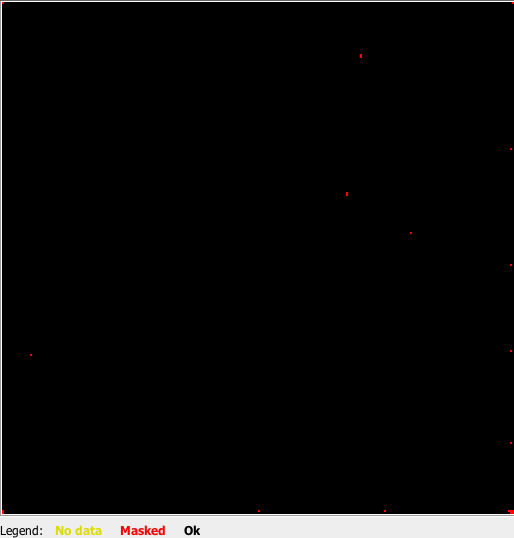
\includegraphics[width=10cm]{figures/calibsw_mask.png}
		\caption{Screenshot kalibračního softwaru - maska špatných pixelů}
		\label{fig:calib:sw_mask}
	\end{center}
\end{figure}

\newpage

%********************************************************************************
% X-ray Calib impl
% > vytvoření kalibrační funkce (+ uložení dat, dodatečné úpravy calib fce, kvalita calib apod.)
%********************************************************************************
\subsection{Vytvoření kalibrační funkce}
Po získání jednotlivých kalibračních bodů je možno přikročit k vytvoření kalibrační funkce pro každý pixel detektoru (viz obr. \ref{fig:calib:sw_calib_function}). Tato úloha spočívá v~proložení kalibračních bodů jednotlivých pixelů kalibrační funkcí \ref{eq:calib:calib_function}, resp. nalezení takových parametrů $a~,b~,c~\text{a}~t$ kalibrační funkce \ref{eq:calib:calib_function} tak, aby součet reziduí byl minimální (viz \ref{calib:sw:spektra}).

\begin{figure}[t]
	\begin{center}
		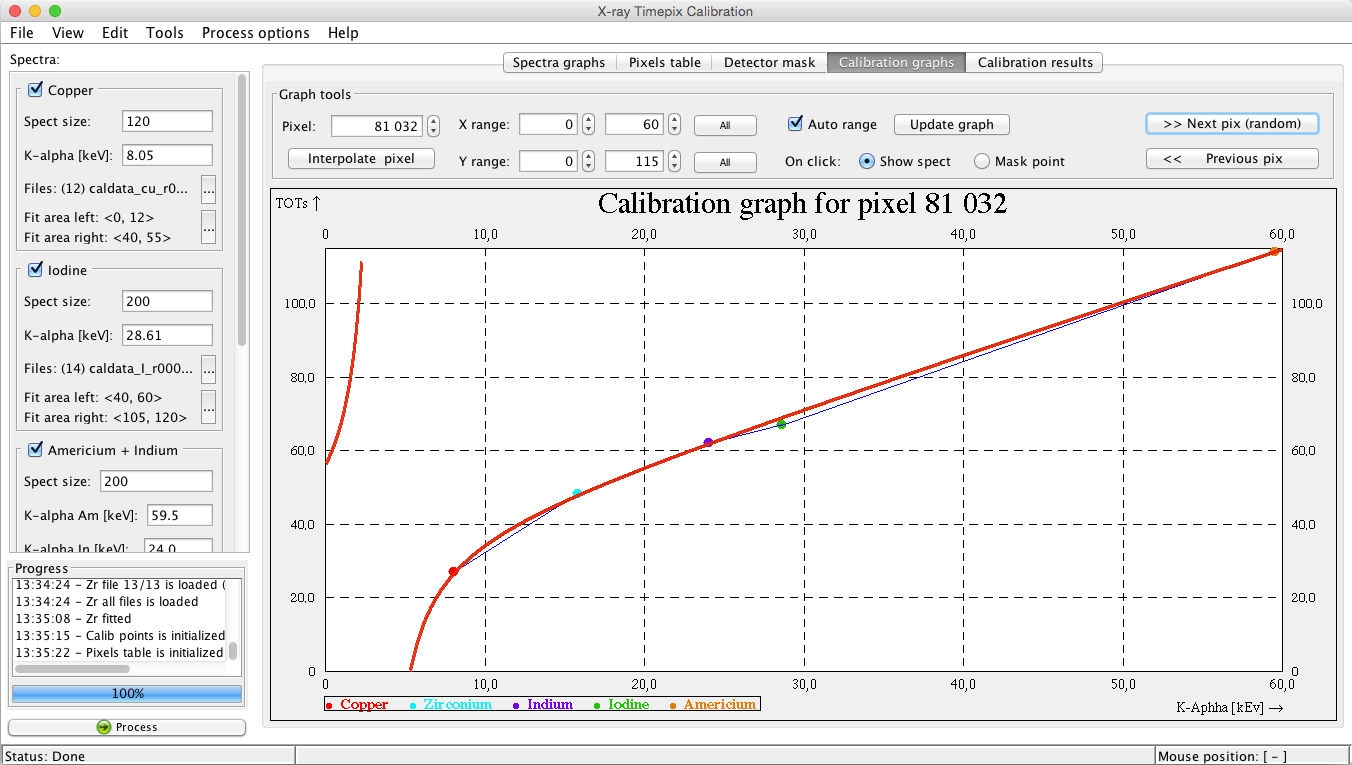
\includegraphics[width=15cm]{figures/calibsw_cc.png}
		\caption{Screenshot kalibračního softwaru - kalibrační funkce}
		\label{fig:calib:sw_calib_function}
	\end{center}
\end{figure}

Jednotlivé parametry kalibrační funkce \ref{eq:calib:calib_function} jsou vzájemně závislé, proto pro nalezení těchto parametrů nelze použít stejný algoritmus, jako při analýze spekter (\ref{calib:sw:spektra}). Tato metoda byla navržena tak, aby byla schopná kalibrační funkci vytvořit ze dvou bodů. Počet kalibračních bodů je variabilní položkou, proto jsou pro nalezení parametrů kalibrační funkce \ref{eq:calib:calib_function} použity různé algoritmy.

\begin{description}
	\item[Algoritmus pro dva body]
	Při kalibraci pomocí dvou kalibračních bodů je uživatel vyzván k~zadání parametrů $c$ a~$t$ kalibrační funkce. Zbylé parametry jsou vypočteny pomocí soustavy rovnic \ref{eq:calib:2points} a~dvou známých kalibračních bodů.
	\begin{eqnarray}\label{eq:calib:2points}
		ax_{1} + b - \frac{c}{x_{1}-t} &=& y_{1} \\
		ax_{2} + b - \frac{c}{x_{2}-t} &=& y_{2} \nonumber 
	\end{eqnarray}
	Při parametrizaci proměnných $c$ a~$t$ vzniká velká nepřesnost, především v~nelineární oblasti nižších energiích, proto je tato metoda pro dva body nejméně přesná.

	\item[Algoritmus pro tři body]
	Tří-bodová kalibrace je oproti dvou-bodové kalibraci značně přesnější. Protože kalibrační funkce má čtyři parametry, je třeba nějaký z~nich parametrizovat. Uživatel je na začátku kalibračního procesu vyzván k~zadání parametru $t$ a~zbylé parametry budou vypočteny ze soustavy rovnic \ref{eq:calib:3points}.
	\begin{eqnarray}\label{eq:calib:3points}
		ax_{1} + b - \frac{c}{x_{1}-t} &=& y_{1} \nonumber \\
		ax_{2} + b - \frac{c}{x_{2}-t} &=& y_{2} \\
		ax_{3} + b - \frac{c}{x_{3}-t} &=& y_{3}\nonumber 
	\end{eqnarray}

	\item[Algoritmus pro čtyři body]
	Algoritmus pro čtyři body je komplikovanější. Nejprve je parametrizován parametr $t$ (bez zásahu uživatele). Poté jsou parametry $a,~b~\text{a}~c$  vypočteny pomocí třech bodů soustavy rovnic \ref{eq:calib:3points}. Tyto tři body jsou vybrány následovně:
	\begin{description}
		\item[1. bod] je vybrán jako bod s~nejnižší energií.
		\item[2. bod] je vybrán z~některého z~prostředních bodů (ve výchozím nastavení 2. bod s~nejnižší energií - možné změnit v~\texttt{Edit > Adjust middle trial point}).
		\item[3. bod] je vybrán jako bod s~nejvyšší energií.
	\end{description}

	Poté pomocí metody bisekce a~metody nejmenších čtverců je nalezena taková hodnota parametru $t$, kdy jeho reziduum je minimální, v~ideálním případě nulové.

	\item[Algoritmus pro pět a~více bodů]
	První část algoritmu pro pět a~více bodů se od algoritmu pro čtyři body nikterak neliší - pomocí třech bodů (volba prostředního je opět na uživateli) jsou vypočteny parametry $a,~b~\text{a}~c$ a~poté pomocí metody bisekce a~čtvrtého bodu je určen parametr $t$. V~ideálním případě prochází funkce \ref{eq:calib:calib_function} všemi čtyřmi body, nebo alespoň jejich rezidua jsou minimální. 

	Pátý bod (popř. další body) je zohledněn pomocí metody bisekce a~metody nejmenších čtverců, přičemž v~rámci jedné iterace tohoto algoritmu se mění všechny parametry (jelikož jsou vzájemně závislé). Postupně je ke každému parametru přičtena konstanta základního kroku a~je sledována se změna sumy reziduí. Z~těchto změn je vytvořen vektor směru změny všech parametrů. Pomocí metody bisekce je přičítán násobek tohoto vektoru (v~jednotlivých krocích) k~parametrům funkce, přičemž je sledována změna sumy reziduí. Daná iterace končí, když se suma reziduí přestane zmenšovat.

	Počet těchto iterací uživatel může opět nastavit v hlavní liště (\texttt{Edit > Set number of iterations}).

\end{description}

Po dokončení procesu kalibrace software nabízí v~záložce \texttt{Calibration graphs} možnost zobrazení kalibrační funkce pro jednotlivé pixely detektoru. Zde je možné jednotlivé pixely interpolovat (více v~\ref{calib:sw:post_process}), nebo kliknutím na daný kalibrační bod zamaskovat, nebo zobrazit jeho spektrum (dle preferencí uživatele). Software rovněž umožňuje hromadné maskování kalibračních bodů ve zvoleném intervalu (\texttt{Tools > Batch calib points masking} v~hlavní liště).

Výstupní data tvoří $a~,b~,c~\text{a}~t$ parametry kalibrační funkce \ref{eq:calib:calib_function}, které je možné uložit (pomocí \texttt{File > Save calib files} v~hlavní liště). Tato data je možné uložit v~samostatných souborech pro každý parametr, kde hodnoty daného parametru pro jednotlivé pixely jsou zapsány v~matici, nebo je možné tato data uložit do jednoho souboru, kde jednotlivé parametry jsou zapsány ve sloupcích.


%********************************************************************************
% X-ray Calib impl
% > Dodatečné úpravy
%********************************************************************************
\subsection{Dodatečné úpravy}\label{calib:sw:post_process}
Tento kalibrační software rovněž nabízí nástroje pro vizualizaci kvality kalibrace. K~tomuto účelu slouží záložka \texttt{Calibration results}, kde v~rámci bočního pohledu na detektor je možné si v~grafu zobrazit všechny hodnoty vybraného parametru kalibrační funkce \ref{eq:calib:calib_function} - viz obr. \ref{fig:calib:sw_calib_results}.

Díky této vizualizaci výsledků kalibrace je možné snadno odhalit případnou deviaci některého z~parametrů pro určitý pixel detektoru. Kalibrační hodnoty je pro takto poškozený pixel možné upravit, například pomocí interpolace hodnot čtyř sousedních pixelů (spojených hranou s~poškozeným pixelem). Pixely je možné interpolovat samostatně, nebo automaticky pomocí nástroje zvaném \texttt{Batch interpolating} (v záložce \texttt{Tools} hlavní lišty), který uživateli umožňuje zvolit rozsah hodnot daného parametru, ve kterém budou všechny pixely interpolovány.

\begin{figure}[t]
	\begin{center}
		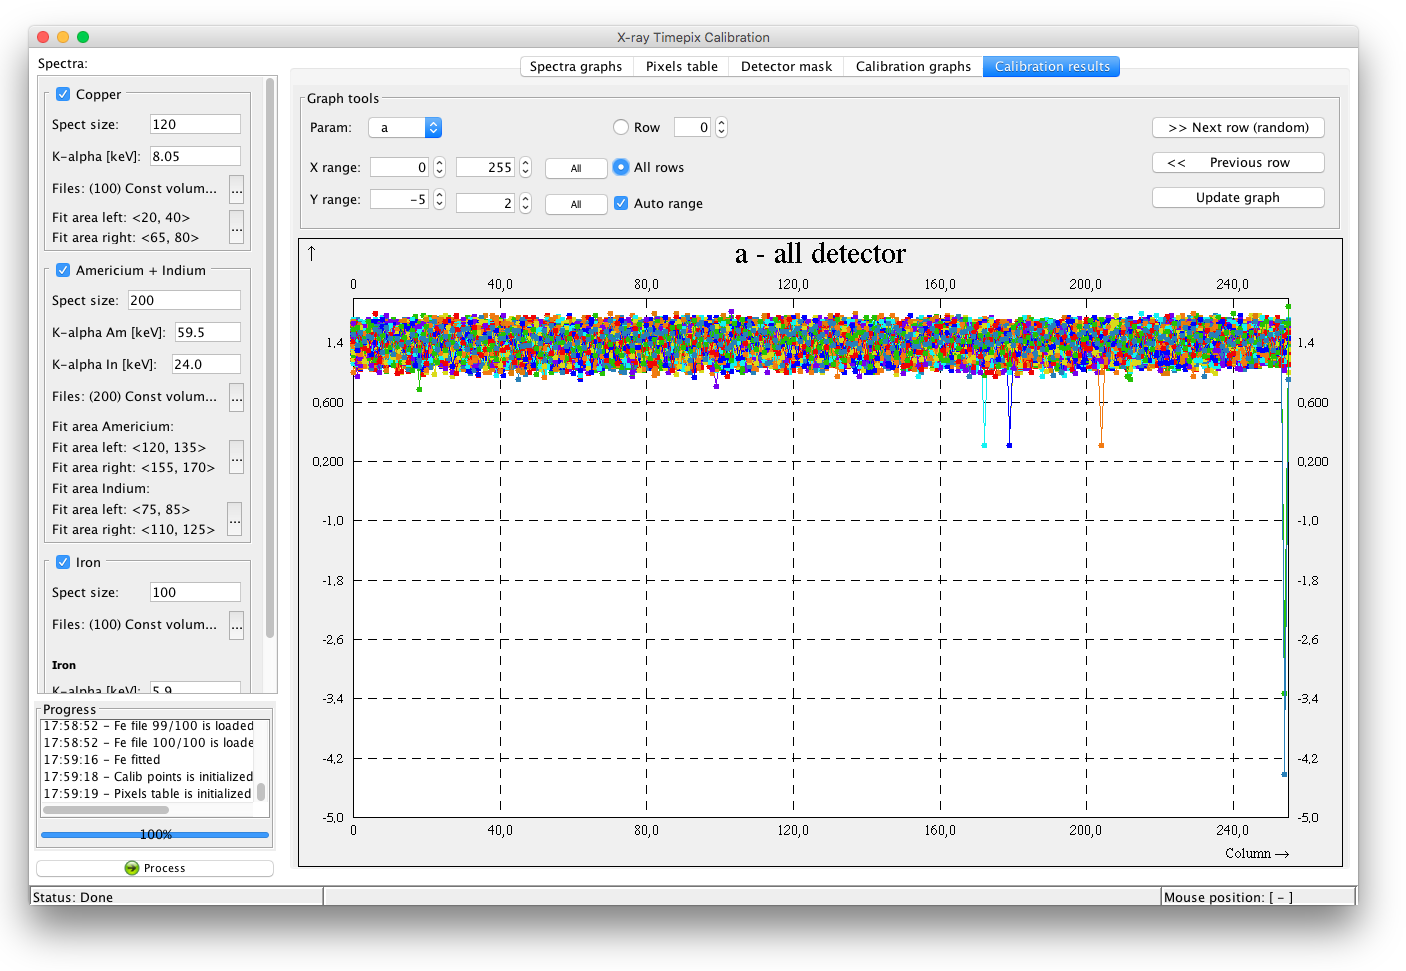
\includegraphics[width=16cm]{figures/calibsw_result.png}
		\caption{Screenshot kalibračního softwaru - vizualizace výsledných parametrů kalibrace v řezu přes řádky detektoru}
		\label{fig:calib:sw_calib_results}
	\end{center}
\end{figure}










\addbibresource{reference.bib}

\chapter{Atlas TPX}\label{atlas}
Atlas TPX, síť 16\footnote{V průběhu LS3\textsuperscript{\ref{ls}} (plánováno 2017 - 2018) je plánováno rozšíření teto sítě o nové detektory} hybridních částicových pixelových detektorů typu Timepix \ref{det:tim}, nainstalovaných na různé pozice experimentu Atlas na LHC\footnote{z angl. Large Hadron Collider} v CERN během LS2\footnote{\label{ls}z angl. long shutdown - dlouhodobá technologická přestávka LHC} (leden 2013 až březen 2015) je následníkem svého předchůdce - sítě Atlas MPX (viz \ref{atlas:mpx}). Hlavní motivací výměny této sítě bylo využití nových technologií, především pak nového detekčního čipu Timepix. Ten na rozdíl od svého předchůdce Medipix2 \ref{det:med} umožňuje rozšíření naměřené informace i o časovou oblast (viz \ref{det:tim}). To nově umožňuje provozovat detektory v módech TOA\footnote{z angl. Time of Arrival - čas příletu částice v hodinových cyklech detektoru od začátku akvizice} a TOT\footnote{z angl. Time Over Treshold - počet hodinových cyklů, kdy komparační napětí je větší, než referenční (ekvivalent energie deponované částice, viz kapitola \ref{calib})}. 

Další změnou oproti svému předchůdci je, že každý detektor obsahuje dva detekční čipy s tloušťkami $300~\mu m$ a $500~\mu m$, umístěné předními stranami k sobě - viz \ref{fig:tpx_detector_layers}. To přináší možnost měřit koincidence - když částice projde oběma vrstvami  detektoru a zároveň v každé nechá jisté měřitelné množství své energie, je detekována oběma vrstvami a je možné zpětně zrekonstruovat její trajektorii. Tyto koincidence se nejsnáze detekují, pokud oba Timepix čipy pracují v módu TOA - jelikož rychlost částic se blíží rychlosti světla, je vysoce pravděpodobné, že zasažené pixely budou mít stejnou hodnotu.


\begin{figure}[th]
	\begin{center}
		\begin{subfigure}{6cm}
			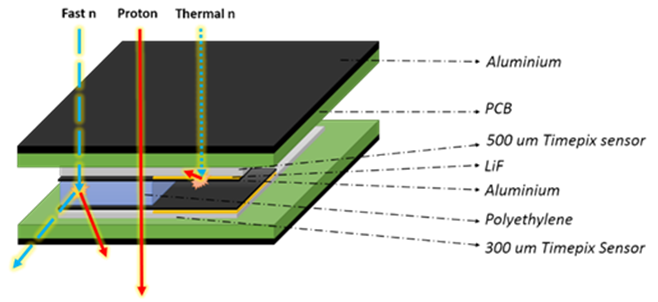
\includegraphics[width=6cm]{figures/tpx_lay.png}	
			\caption{Vrstvy detektoru}
			\label{fig:tpx_detector_layers}
		\end{subfigure}
		\hspace{0.5cm}
		\begin{subfigure}{5cm}
			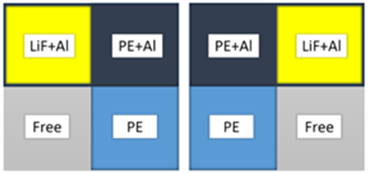
\includegraphics[width=5cm]{figures/tpx_conv.png}
			\caption{Rozmístění konvetorů}
			\label{fig:tpx_detector_convertors}
		\end{subfigure}
		\caption{Atlas TPX detektor - vrstvy a rozmístění konvertorů}
		\label{fig:tpx_detector}
	\end{center}			
\end{figure}

Mezi vrstvami detektoru je umístěn konvertující materiál pro detekci termálních a rychlých neutronů. Rozmístění těchto konvertorů je na obrázku \ref{fig:tpx_detector_convertors}.

Hlavním úkolem Atlas TPX experimentu je online monitorování spektrálních charakteristik velice různorodého radiačního prostředí Atlas experimentu, založené na prostorovém uspořádání sítě a (vzhledem k aktuálním módu detektoru) i na informaci o deponované energii zainteragovaných částic, či na času jejich interakce. 


Detektory, instalované blízko interakčnímu bodu, jsou rovněž použity jako monitory integrované luminozity, což je veličina, která udává počet realizovaných srážek, resp. s intenzitou svazku urychlovače. Podle \cite{wagner:o_lhc} je to veličina, která v případě srážení dvou proti sobě letících svazků ukazuje, jaký je součin počtů částic v jednotlivých svazcích prolétajících jednotkovou plochou v srážkové oblasti, vynásobený počtem obletů svazků za jednotku času (nejčastěji se vyjadřuje v jednotkách na centimetr čtvereční a sekundu).

\begin{figure}[ht]
	\begin{center}
		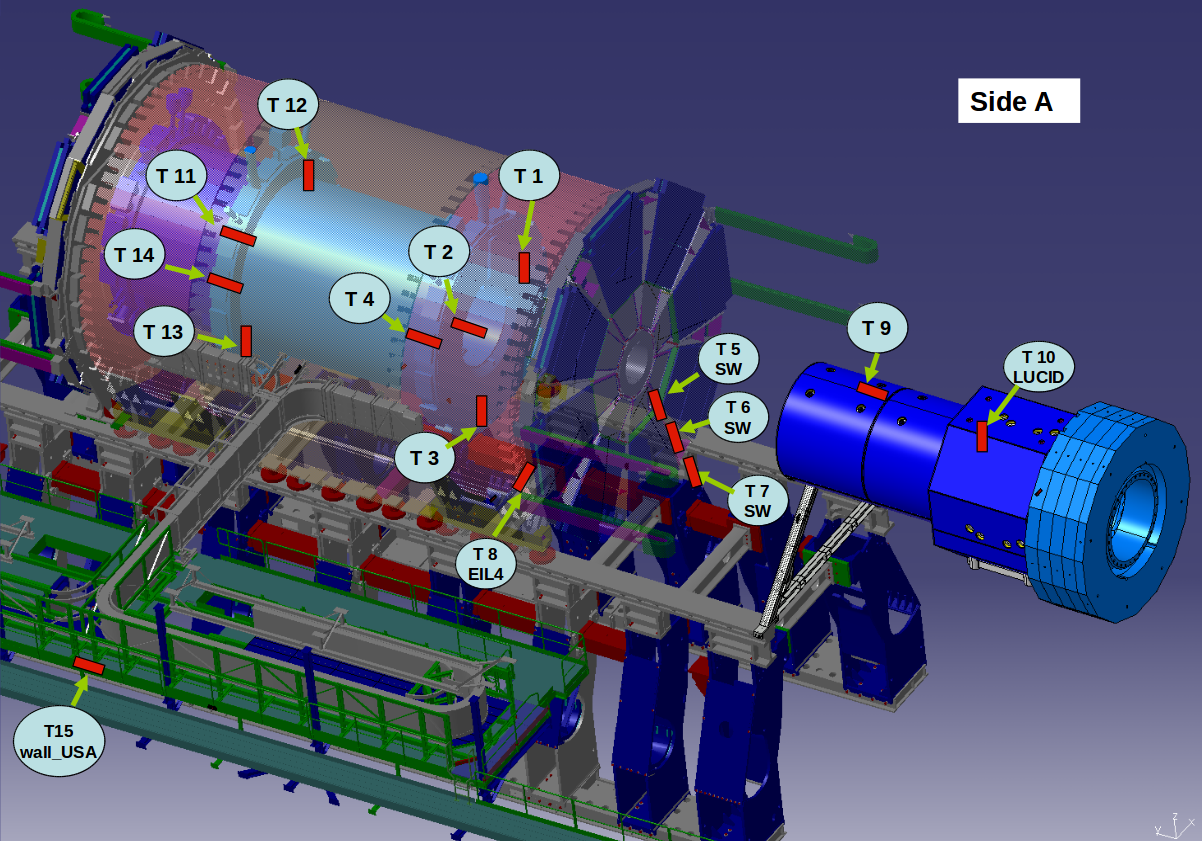
\includegraphics[width=12cm]{figures/tpx_positions.png}
		\caption{Atlas TPX - přehledem rozmístění detektorů}
		\label{fig:tpx_positions}
	\end{center}
\end{figure}

%********************************************************************************
% Atlas MPX
%********************************************************************************
\section{Atlas MPX}\label{atlas:mpx}
Atlas MPX\cite{Vykydal200935}\cite{atlasmpx} je předchůdcem detektorové sítě Atlas TPX, který je v současné době plně nahrazen. Detektorová síť Atlas MPX se skládala z 16 Medipix2 detektorů, které byly instalovány na různé pozice Atlas detektoru. Hlavním cílem této sítě bylo měření vlastností radiačního pole uvnitř experimentu Atlas, jeho složení, spektroskopických charakteristik a částečně také přispěla k měření neutronů. 


Všechny detektory operovaly v tzv. \texttt{Medipix módu}, který se vyznačuje tím, že v rámci jedné akvizice počítá počet částic, které interagovaly pixelovou maticí detektoru a jejichž deponovaná energie byla vyšší, než prahová. Na obrázku \ref{fig:mpx_cluster} je znázorněn snímek z jednoho detektoru s detailem zachycených částic. Na obrázku vpravo nahoře je částice typu \texttt{heavy blob} (těžce nabitá částice, jejíž trajektorie byla kolmá s povrchem detektoru), vpravo dole je pak zachycena částice typu \texttt{heavy track} (také těžce nabitá částice, která ale přiletěla pod větším a proto zanechala větší stopu) - více klasifikaci částic se dočtete v podkapitole \ref{atlas:sw_arch}.


\begin{figure}[ht]
	\begin{center}
		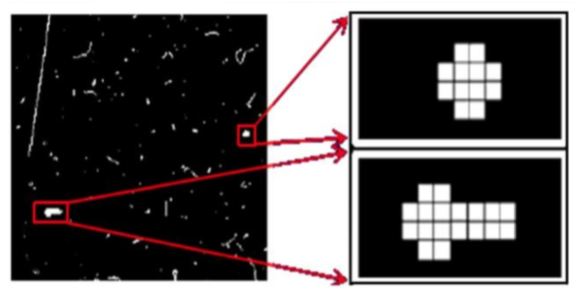
\includegraphics[width=7cm]{figures/mpx_cluster.png}
		\caption{Snímek z Atlas MPX detektoru s výřezem zachycených částic (převzato z \cite{atlasmpx})}
		\label{fig:mpx_cluster}
	\end{center}
\end{figure}


Každý z těchto detektorů byl osazen $300~\mu m$ tlustým křemíkovým senzorem, který byl pokryt konvertory pro lepší detekční účinnost neutronů (obr. \ref{fig:mpx_lay}).

\begin{figure}[ht]
	\begin{center}
		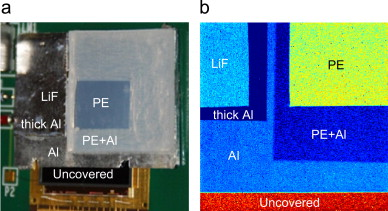
\includegraphics[width=7cm]{figures/mpx-layers.jpg}
		\caption{Fotografie znázorňující Medipix2 detektor s neutronovými konvertory (převzato z \cite{Vykydal200935})}
		\label{fig:mpx_lay}
	\end{center}
\end{figure}

\subsection{Hardwarová a softwarová architektura sítě Atlas MPX}
Tato síť se skládala z 16 \texttt{Medipix2} \ref{det:med} detektorů, které byly pomocí USB vyčítacího rozhraní \texttt{FITPix} \ref{det:fitpix} připojeny ke třem počítačům (z důvodu distribuce toku dat a výkonu). Na každém počítači se o komunikaci s detektory staral software \texttt{Pixelman} \ref{det:pixelman}, který řídil akvizici dat, nastavování parametrů detektorů apod. 

Pro vzdálené obládání byl vyvinut plugin pro Pixelman, který umožňoval jeho rozšíření o TCP/IP ovládací vrstvu. Pomocí jednoduchého textového protokolu bylo tedy možné řídit každý ze třech uzlů. Pro tyto účely byla vyvinuta centrální řídící aplikace \cite{Turecek2011S45}, pomocí které bylo možné řídit řídit akvizici všech detektorů a nastavovat jejich parametry. Tato aplikace poskytovala webové rozhraní (obr. \ref{fig:mpx_web}), které díky tou dobou méně striktní CERNské politice síťové bezpečnosti bylo možné tento experiment ovládat odkudkoliv z internetu.

\begin{figure}[ht]
	\begin{center}
		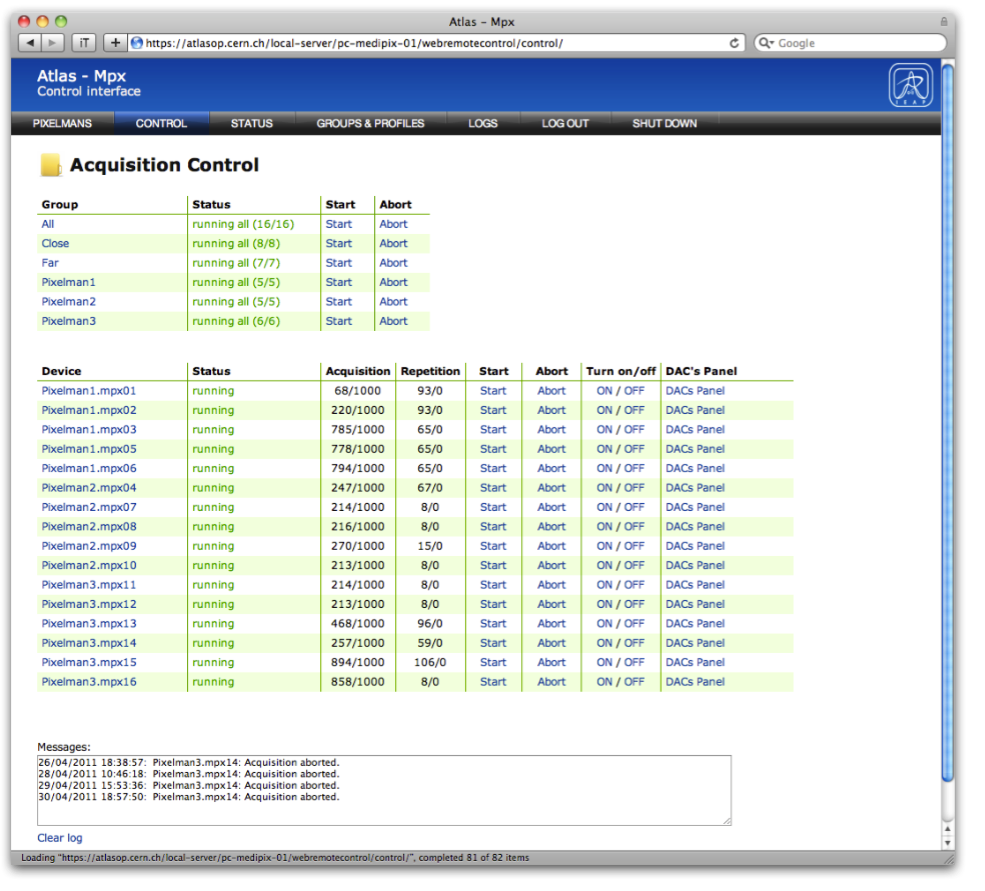
\includegraphics[width=10cm]{figures/mpx_web.png}
		\caption{Atlas MPX - řídící aplikace (převzato z \cite{TurecekThesis2011})}
		\label{fig:mpx_web}
	\end{center}
\end{figure}

%********************************************************************************
% Hardwarová architektura
%********************************************************************************
\section{Hardwarová architektura}\label{atlas:hw_arch}
Při návrhu hardwarové architekty sítě Atlas TPX musela být zohledněna zvýšená intenzita radiačního a elektromagnetického pole v prostorách Atlas detektoru. Snahou proto bylo, co nejvíce hardwarových komponent umístit z dosahu tohoto pole. Z pohledu hardwarové instalace této detektorové sítě se prostory Atlas experimentu dělí na dvě části - \texttt{UX15} a \texttt{USA15} (viz obr. \ref{fig:tpx_hw_diagram}). V \texttt{UX15} se nachází vlastní experiment. V tomto prostoru byly umístěny jen detektory (na obr. \ref{fig:tpx_hw_diagram} \texttt{TPX01} až \texttt{TPX15}) a zbytek sítě byl instalován v \texttt{USA15}, kterou od zbytku experimentu dělí cca $60~m$ tlustá železobetonová stěna. Tady se nachází vyčítací elektronika a další nezbytný hardware.

\begin{figure}[t]
	\begin{center}
		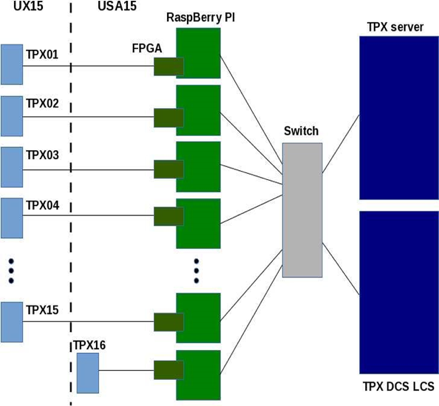
\includegraphics[width=6cm]{figures/tpx_hw_diagram.png}
		\caption{Atlas TPX - diagram hw komponent}
		\label{fig:tpx_hw_diagram}
	\end{center}
\end{figure}

Na obrázku \ref{fig:tpx_hw_foto} je fotografie  těchto komponent. Jak již bylo zmíněno výše, detektor (z obr. \ref{fig:tpx_hw_foto}, na obr. \ref{fig:tpx_hw_diagram} jako \texttt{TPX01} až \texttt{TPX15}) se skládá z dvojice detekčních čipů \texttt{Timepix}, které jsou pomocí \texttt{LVDS} zesilovačů a cca $100~m$ dlouhých ethernetových kabelů propojeny se zařízením \texttt{AtlasPix} (obr. \ref{fig:tpx_hw_foto} dole), které vzniklo modifikací vyčítacího rozhraní \texttt{FITPix} \ref{det:fitpix}. Toto zařízení obsahuje \texttt{FPGA}\footnote{z angl. Field Programmable Gate Array (programovatelné hradlové pole)}, minipočítač \texttt{Raspberry Pi} a další podpůrnou elektroniku. 

\texttt{FPGA} se stará o komunikaci s \texttt{Timepix} detektory, v rámci které dochází k nastavování řídících registrů \texttt{Timepix} čipů, ovládání akvizice, vyčítání dat, řízení triggeru\footnote{řídící signál, který spouští resp. zastavuje (dle konfigurace) akvizici detektoru} apod.

\begin{figure}[t]
	\begin{center}
		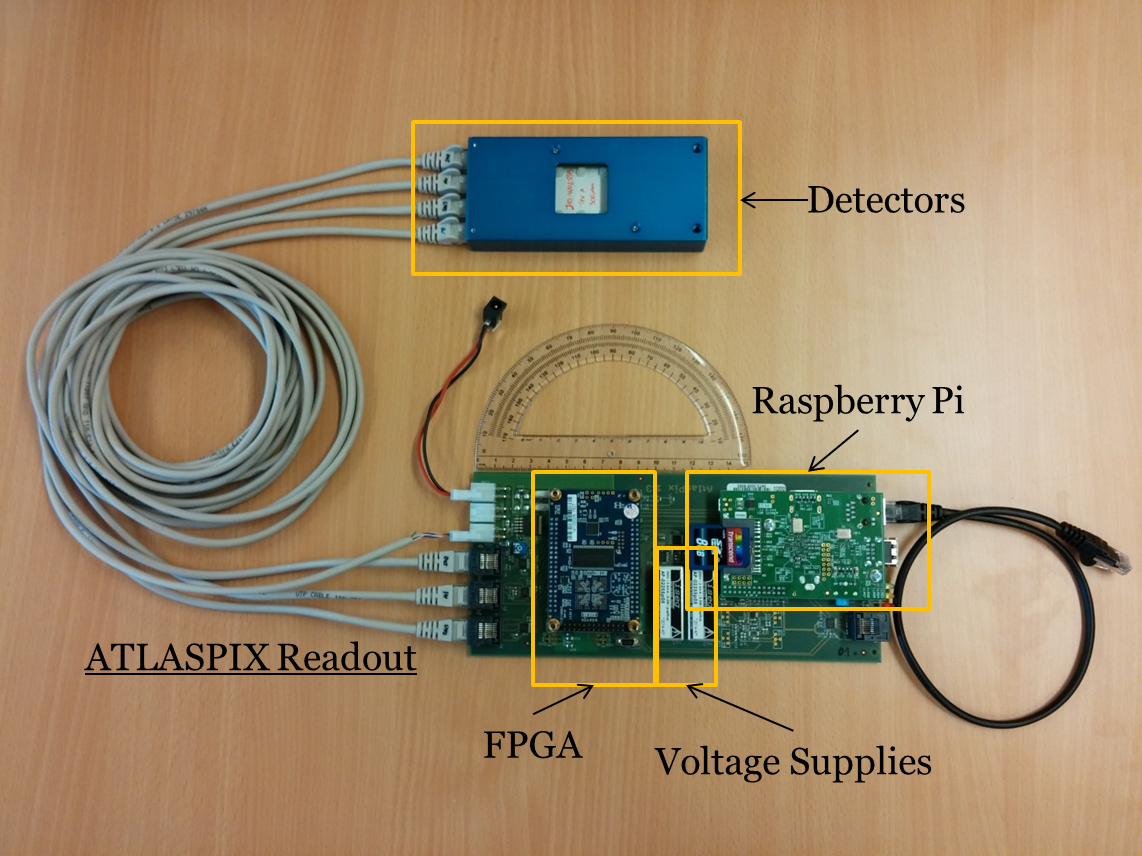
\includegraphics[width=8cm]{figures/tpx_hw_foto.png}
		\caption{Atlas TPX - fotografie hw komponent}
		\label{fig:tpx_hw_foto}
	\end{center}
\end{figure}

Dalším článkem tohoto řetězce je minipočítač \texttt{Raspberry Pi}, který plní dvě úlohy. Tou první je komunikace s \texttt{FPGA} pomocí \texttt{SPI}\footnote{z angl. Serial Peripheral Interface (sériové periferní rozhraní)} rozhraní a deserializace (získání dat ze struktury komunikačního protokolu) a derandomizace (není zaručena časová posloupnost) surových dat z \texttt{FPGA}. Druhou úlohou tohoto zařízení je poskytování API\footnote{z angl. Application Programming Interface (aplikační programovací rozhraním)} vyšším řídícím vrstvám této sítě pomocí specifikovaného komunikačního protokolu a klasického ethernetového rozhraní.

Všechny tyto zařízení jsou pomocí ethernetového switche propojeny s \texttt{TPX serverem}, centrálním bodem této sítě, který jí pomocí řídícího softwaru \ref{atlas:cont} a komunikačního protokolu \ref{atlas:cont:det} ovládá. Zároveň je k síti připojen i \texttt{TPX DCS\footnote{z angl. Data Control System} server}, pomocí kterého jsou různé stavové informace \texttt{Atlas TPX} sítě předávány CERNu, resp. Atlas experimentu. Tyto stavové informace jsou převážně hardwarového charakteru (na př. napětí, časování apod.), ale také jsou předávána data o počtu pořízených snímků, jejich okupanci apod.

%********************************************************************************
% Softwarová architektura
%********************************************************************************
\section{Softwarová architektura}\label{atlas:sw_arch}
Na obrázku \ref{fig:tpx_sw_diagram} je znázorněn diagram návrhu softwarové architektury sítě Atlas TPX z pohledu jejího řízení, vizualizace dat a předávání stavových informací CERNu. Diagram je členěn do dvou základních částí - ATCN\footnote{z angl. ATLAS Technical Control Network} (technická síť Atlas experimentu, která je oddělena od zbytku Atlas sítě a obsahuje systémy pro vyčítání dat a pro řízení, včetně TDAQ\footnote{z angl. Trigger and Data Aquisition (trigger a akvizice dat)} a DSC \cite{Ballestrero:atlas_network_upgrade}) a CERN služby, které poskytují perzistentní úložiště dat a web server pro jejich vizualizaci.

\begin{figure}[th]
	\begin{center}
		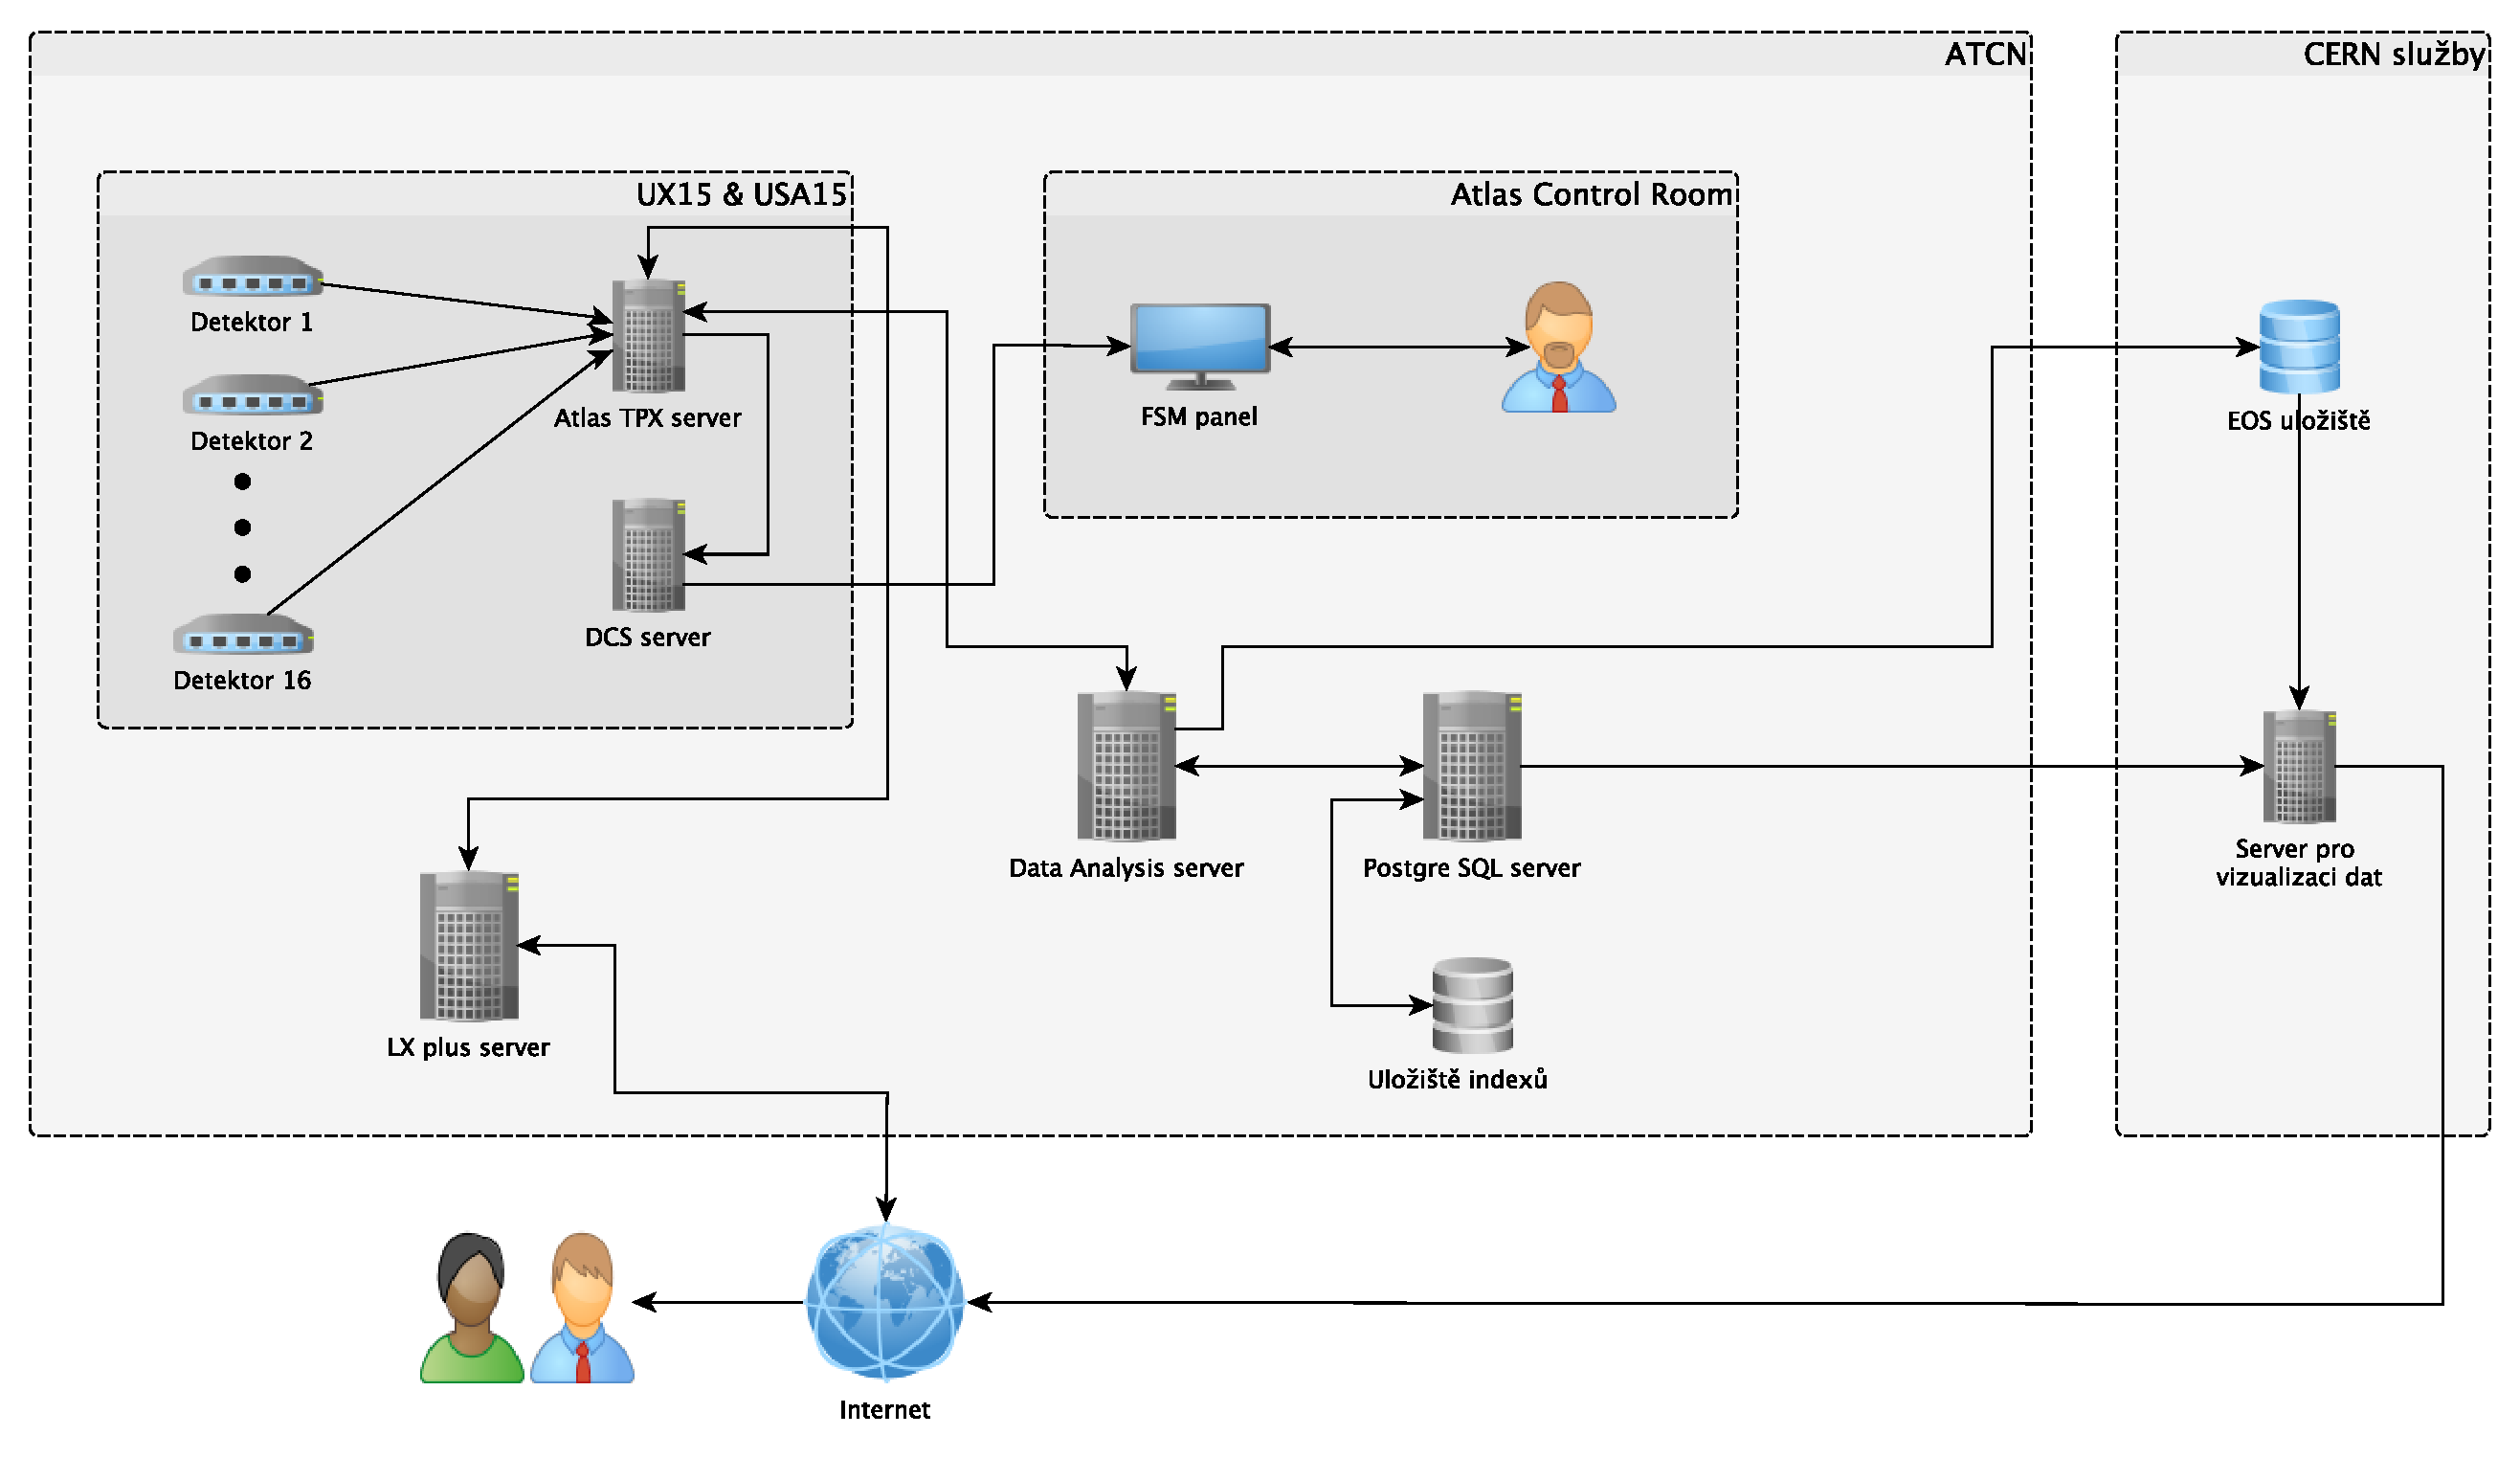
\includegraphics[width=16cm]{figures/atlas_tpx_sw_diagram.pdf}
		\caption{Atlas TPX - diagram softwarových komponent}
		\label{fig:tpx_sw_diagram}
	\end{center}
\end{figure}

\begin{description}
	\item[Popis architektury z pohledu řízení:] 
		Na obrázku \ref{fig:tpx_sw_diagram} se nachází Atlas TPX server, který je umístěn v serverové místnosti (USA15) Atlas experimentu, umístěné cca $100~m$ pod zemským povrchem. Tento server pomocí komunikačního protokolu (specifikovaném v \ref{atlas:cont:det}) řídí činnost detektorů (nastavování parametrů, ovládání akvizice apod.). Zároveň pomocí JSON REST API poskytuje rozhraní pro své řízení a předávání stavových informací (více v \ref{atlas:cont:api}). Díky tomuto rozhraní je možné činnost serveru řídit z ATCN sítě. Pro potřeby vzdáleného ovládání mimo síť ATCN slouží \texttt{LX plus server}, který zajistí spojení vytvořením SSH tunelu.\\
		Předávání stavových informací zajišťuje \texttt{DCS server}, který je od \texttt{Atlas TPX serveru} získává pomocí jeho API. Hlavním úkolem DCS je zajištění získávání stavových informací ze všech experimentů a detektorů homogenním způsobem a interakce s LHC (předávání dat luminozitě, stavu svazku urychlovače, radiační pozadí apod.). Tato data jsou dále předávána do Atlas Control Room, která se nachází na povrchu. Tam jsou tato data operátorů prezentována pomocí \texttt{FSM} panelu, což je aplikace, která vizualizuje stromovou strukturu všech systému a detektorů Atlas experimentu. Každý list této stromové struktury (detektor, senzor atd.) má několik proměnných, z nichž každá má předem definované intervaly s příslušnými stavy (\texttt{OK}, \texttt{WARNING}, \texttt{ERROR}, \texttt{FATAL} atd.). Výhodou této struktury je, že pokud kterýkoliv list změní svůj stav, tak se tato informace propaguje přes všechny nadřazené uzly, tudíž odhalení případné chyby je pro operátory mnohem snazší.
	\item[Popis architektury z pohledu analýzy a vizualizace dat:] 
		Když kterýkoliv detektor dokončí akvizici snímku, tak vygeneruje a pošle asynchronní událost \texttt{Atlas TPX serveru} s informací, že data jsou připravena k vyčtení. Následně server vyčte snímek z detektoru (i s jeho metadaty), zpracuje a připojí k němu informace o nastavení detektoru. Poté je třeba data přenést do \texttt{Data analysis serveru}, což v principu je možné dvěma\footnote{V současné době je možný pouze první způsob, protože díky politice CERNské síťové bezpečnosti a dlouhými schvalovacími termíny je Data analysis server a všechny s ním související systémy (web server, databáze s indexem a vlastní úložiště dat) prozatím umístěn v ÚTEF ČVUT v Praze.} způsoby:
		\begin{enumerate}
			\item \texttt{Atlas TPX server} uloží získaná data v textové podobě do lokálního (či síťového) datového úložiště, odkud jsou přenesena do \texttt{Data analysis serveru} pomocí automatického kopírovacího skriptu.
			\item Druhou možností je přenesení dat pomocí JSON REST API protokolu, který je \texttt{Data analysis serverem} implementován. Tento druhý způsob je výhodnější, neb minimalizuje prodlevu mezi dobou pořízení snímku a následném zpracováním \texttt{Data analysis serverem} a dostupnosti jeho vizualizace pomocí web serveru a zároveň přináší úsporu objemu přenesených dat.
		\end{enumerate}
		Hlavní úlohou \texttt{Data analysis serveru} je provedení tzv. Cluter analýzy. Jde o proces, při kterém jsou z každého snímku získány shluky sousedních pixelů (tzv. clusterů), které mají nenulovou hodnotu. Z těchto clusterů, resp. z jejich tvaru a celkové deponované energie částice (pokud zasažení pixely operovaly v TOT módu) je možné zjistit typ částice, která danou událost způsobila. Na obrázku \ref{fig:tpx_ca} můžete vidět 6 základních dělení clusterů, kde
		 \begin{enumerate}[label=(\alph*)]
			\item je tzv. \texttt{DOT}, způsobený fotony, či elektrony o energii do $10~keV$
			\item je tzv. \texttt{SMALL BLOB}, způsobený fotony, či elektrony s energií vetšinou nad $10~keV$
			\item je tzv. \texttt{CURLY TRACK}, způsobený elektrony do $10~MeV$
			\item je tzv. \texttt{HEAVY BLOBS}, způsobený těžce nabitými částicemi (na př. alfa)
			\item je tzv. \texttt{HEAVY TRACK}, způsobený těžce nabitými částicemi (na př. protony)
			\item je tzv. \texttt{STAIGHT TRACK}, způsobený těžce nabitými částicemi (muony apod.)
		\end{enumerate}
		Po dokončení analýzy dat, jsou data uložena do \texttt{ROOT}\footnote{\url{https://root.cern.ch/}} souborů (do souborové struktury po detektorech a hodinách). \texttt{ROOT} je framework, který je vyvíjen v CERN a je určený pro ukládání dat a jejich analýzu. Vygenerované soubory jsou ukládány do \texttt{EOS úložiště}, což je služba pro perzistentní ukládání \texttt{ROOT} souborů provozovaná CERN.\\
		Jelikož každý \texttt{ROOT} soubor má velikost řádově v jednotkách $GB$, jakékoliv operace nad nimi (na příklad vyhledávání) jsou velice časově náročné. Z tohoto důvodu vznikla \texttt{PostgreSQL} databáze s indexem na jednotlivé clustery, obsažené v \texttt{ROOT} souborech. 
		Pro vizualizaci dat slouží web server, který pomocí databáze s indexem a \texttt{ROOT} souborů poskytuje online výsledky cluster analýzy a další informace.
\end{description}

\begin{figure}[t]
	\begin{center}
		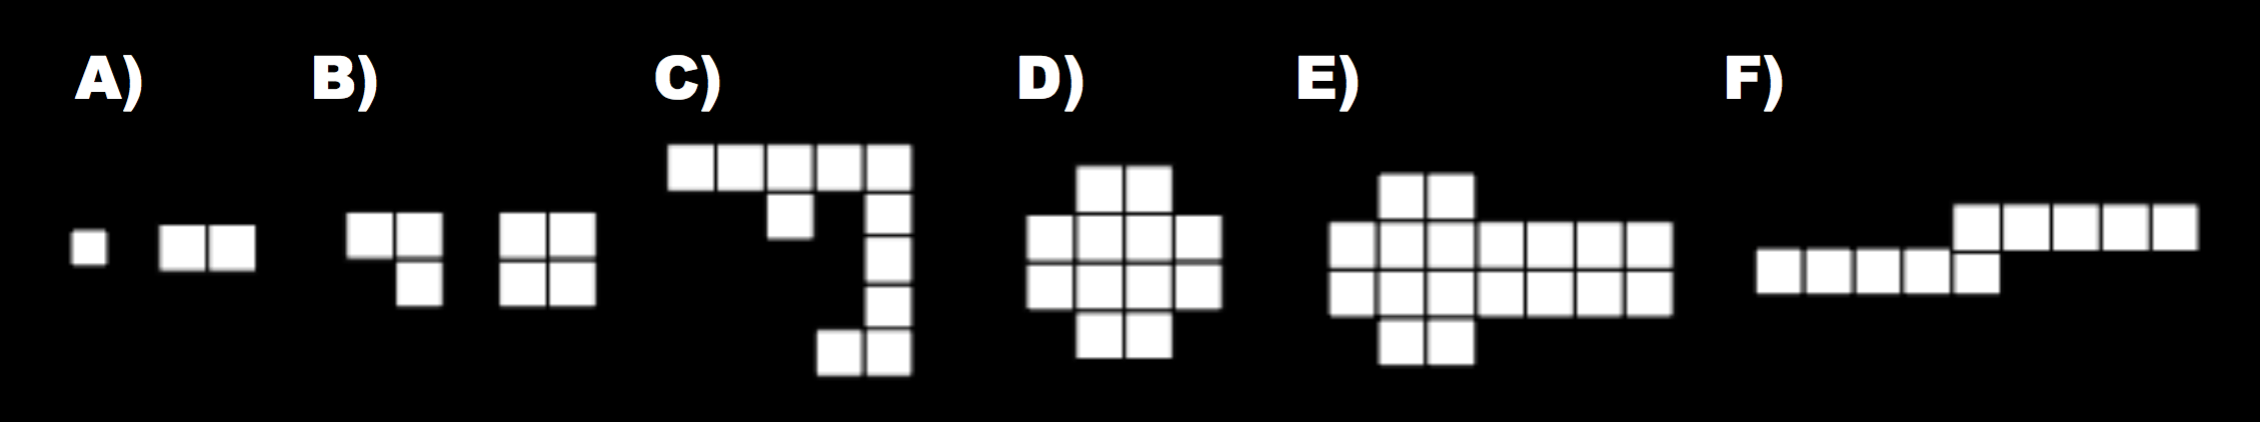
\includegraphics[width=10cm]{figures/ca.png}
		\caption{Cluster analýza - 6 základních typů clusterů (převzato z \cite{TurecekThesis2011})}
		\label{fig:tpx_ca}
	\end{center}
\end{figure}


%********************************************************************************
% Řídící software a jeho implementace
%********************************************************************************
\section{Řídící software a jeho implementace}\label{atlas:cont}
Tato kapitola je věnována návrhu a implementaci řídícího software sítě Atlas TPX, který je nasazen na Atlas TPX serveru (viz obr. \ref{fig:tpx_sw_diagram}). Úkolem  tohoto software se zajištění komunikace s detektory, zejména pak řízení akvizice, nastavování parametrů a vyčítání dat - tato komunikace bude popsána v kapitole \ref{atlas:cont:det}. Další úlohou tohoto software je poskytování rozhraní pro řízení své činnosti a pro předávání stavových informací o Atlas TPX síti. Toto rozhraní je implementováno pomocí \texttt{JSON REST API} a detailně bude popsáno v kapitole \ref{atlas:cont:api}. \todo

%********************************************************************************
% Řídící software a jeho implementace - Řízení detektorů
%********************************************************************************
\subsection{Řízení detektorů}\label{atlas:cont:det} % + komunikační protokol
Jak již bylo zmíně výše, detektor se skládá ze dvou \texttt{Timepix} detekčních čipů, \texttt{FPGA} a minipočítače \texttt{Raspberry Pi}, který implementuje komunikační protokol, díky kterému umožňuje řídícímu software ovládání činnosti detektoru. V podkapitole \ref{atlas:cont:det:comunikacni_protokol} naleznete popis tohoto komunikačního protokolu.

%********************************************************************************
% Řídící software a jeho implementace - Řízení detektorů
% > Komunikační protokol
%********************************************************************************
\subsubsection{Komunikační protokol}\label{atlas:cont:det:comunikacni_protokol}
Tabulka \ref{tab:com_packet} znázorňuje strukturu komunikačního rámce (tzv. paketu) tohoto protokolu pomocí posloupnosti bytů z pohledu Atlas TPX serveru, resp. z pohledu řídícího software. V horní části se nachází struktura odchozího paketu, kde:
\begin{description}
	\item[0x55]\footnote{\label{hexa}značení v hexadecimální soustavě} je tzv. \texttt{START BYTE}, který značí začátek paketu,
	\item[CMD] je typ příkazu (tzv. \texttt{COMMAND TYPE}) - viz tabulka přehledu příkazů \ref{tab:commands},
	\item[SIZE 1..4] je pole vždy o velikosti čtyřech bytů značících velikost (resp. počet bytů) položky \texttt{DATA}, zakódovaných v \texttt{BIG ENDIAN},
	\item[DATA 1 .. DATA n] je pole vlastních přenesených dat o velikosti $n$,
	\item[0xAA] \texttt{STOP BYTE}, který značí konec paketu.
\end{description}
Struktura odchozího paketu je velice podobná, až na byte \texttt{ERR}, který oproti příchozího paketu obsahuje. Tento byte může nabývat hodnoty 0x00 (když zpracování požadavku serveru detektorem proběhlo bet chyby), nebo 0x01 (jinak).

\begin{table}[th]
	\begin{center}
		\begin{bytefield}[bitwidth=1.35cm]{8}
			%\bitheader{0-8} \\
			\begin{rightwordgroup}{odchozí\\paket}
				\bitbox{1}{0x55} & \bitbox{1}{CMD} 
				& \bitbox{1}{SIZE 1} & \bitbox{1}{SIZE 2} & \bitbox{1}{SIZE 3} & \bitbox{1}{SIZE 4}
				& \bitbox{3}{DATA 1 .. DATA $n$} & \bitbox{1}{0xAA}
			\end{rightwordgroup} \\ \\ 
			%\bitheader{0-9} \\
			\begin{rightwordgroup}{příchozí\\paket}
				\bitbox{1}{0x55} & \bitbox{1}{CMD} & \bitbox{1}{ERR}
				& \bitbox{1}{SIZE 1} & \bitbox{1}{SIZE 2} & \bitbox{1}{SIZE 3} & \bitbox{1}{SIZE 4}
				& \bitbox{3}{DATA 1 .. DATA $n$} & \bitbox{1}{0xAA}
			\end{rightwordgroup}
			\end{bytefield}
	\end{center}
	\caption{Komunikační protokol - struktura paketů z pohledu serveru}
	\label{tab:com_packet}
\end{table}

\begin{table}[th]
	\begin{center}
		\begin{tabular}{|c|l|}
			\hline
			\textbf{Hodnota příkazu} & \textbf{Název příkazu} \\
			\hline
			0x01 & Ping \\
			\hline
			0x02 & Get status of the detector \\
			\hline
			0x03 & Reset of the device \\
			\hline
			0x04 & Set Bias and Timepix Clock \\
			\hline
			0x05 & Get Bias and Timepix Clock \\
			\hline
			0x06 & Set Pixel Configuration \\
			\hline
			0x07 & Get Pixel Configuration \\
			\hline
			0x08 & Set DAC \\
			\hline
			0x09 & Get DAC \\
			\hline
			0x0A & Perform Digital Test \\
			\hline
			0x0B & Perform Acquisition \\
			\hline
			0x0C & Readout Measured Data \\
			\hline
			0x0D & Direct FITPix Command \\
			\hline
			0x0E & Stop acquisition \\
			\hline
			0xFD & Asynchronous Event from device \\
			\hline
			0xFE & Reboot device \\
			\hline
			0xFF & Shut down \\
			\hline
			\end{tabular}
	\end{center}
	\caption{Komunikační protokol - přehled příkazů}
	\label{tab:commands}
\end{table}

%********************************************************************************
% Řídící software a jeho implementace - Řízení detektorů
% > Popis příkazů komunikačního protokolu
%********************************************************************************
\subsubsection{Popis příkazů komunikačního protokolu}
Následuje struční popis příkazů komunikačního protokolu z pohledu obsahu vlastních přenesených dat odchozího a příchozího paketu (viz tabulka \ref{tab:com_packet})

\begin{description}
	\item[0x01 - Ping]:
		Příkaz pro ověření spojení s detekorem. Na základě rozdílu času odeslání a přijetí paketu je vypočtena prodleva spojení v $ns$ (tzv. ping)
		\begin{description}
			\item[Odchozí data:] nic
			\item[Příchozí data:] nic
		\end{description}
	\item[0x02 - Get status of the detector]:
		Příkaz pro zjištění stavu detektoru.	
		\begin{description}
			\item[Odchozí data:] nic
			\item[Příchozí data ($2~B$):] GST MST
				\begin{itemize}
					\item GST - General Status (obecný status)
						\begin{itemize}
							\item 0x00 - Ok
							\item 0x01 - Chyba detekčního čipu
							\item 0x02 - Obecná chyba
						\end{itemize}
					\item MST - Measurement Status (měřící status)
						\begin{itemize}
							\item 0x00 - Nečinný
							\item 0x01 - Probíhá akvizice
							\item 0x02 - Čekání na trigger
							\item 0x03 - Data připravena k vyčtení
							\item 0x04 - Chyba akvizice
						\end{itemize}
				\end{itemize}
		\end{description}
	\item[0x03 - Reset of the device]:
		Tento příkaz slouží pro vyresetování \texttt{FPGA} a dalších řídících struktur detektoru.
		\begin{description}
			\item[Odchozí data:] nic
			\item[Příchozí data:] nic
		\end{description}
	\item[0x04 - Set Bias and Timepix clock]:
		Příkaz nastavující napětí (Bias) na obou Timepix čipech a jejich meřící frekvenci (Timepix clock)
		\begin{description}
			\item[Odchozí data ($24~B$):] BIAS1($8~B$) BIAS2($8~B$) CLK($8~B$)
				\begin{itemize}
					\item BIAS1, BIAS2 - hodnota napětí pro Timepix čipy (zakódovaná jako 64-bitové double-precision číslo dle standartu \texttt{IEEE 754})
					\item CLK - Měřící frekvence obou Timepix čipů (zakódovaná jako 64-bitové double-precision číslo dle standartu \texttt{IEEE 754})
				\end{itemize}
			\item[Příchozí data:] nic
		\end{description}
	\item[0x05 - Get Bias and Timepix clock]:
		Příkaz pro vyčtení úrovně napětí z obou Timepix čipů a jejich meřící frekvenci
		\begin{description}
			\item[Odchozí data:] nic
			\item[Příchozí data ($24~B$):] BIAS1($8~B$) BIAS2($8~B$) CLK($8~B$)
				\begin{itemize}
					\item BIAS1, BIAS2 - hodnota napětí pro Timepix čipy (zakódovaná jako 64-bitové double-precision číslo dle standartu \texttt{IEEE 754})
					\item CLK - Měřící frekvence obou Timepix čipů (zakódovaná jako 64-bitové double-precision číslo dle standartu \texttt{IEEE 754})
				\end{itemize}
		\end{description}
	\item[0x06 - Set Pixel Configuration]:
		Příkaz pro nastavení konfigurace pro každý pixel detektoru
		\begin{description}
			\item[Odchozí data ($(1+(65536~nebo~2*65536))~B$):] TYPE($1~B$) PIXCFG($(65536~nebo~2*65536)~B$)
				\begin{itemize}
					\item TYPE - Výběr čipu, pro který je konfigurace určena
						\begin{itemize}
							\item 0x00 - Konfigurace určena oboum čipům (délka PIXCFG je $2*65536~B$)
							\item 0x01 - Konfigurace určena prvnímu čipu (délka PIXCFG je $65536~B$)
							\item 0x02 - Konfigurace určena druhému čipu (délka PIXCFG je $65536~B$)
						\end{itemize}
					\item PIXCFG - Pole konfiguračních bytů (každý byte je pro jeden pixel) pro jednotlivé pixely. Délka tohoto pole je závyslá na parametru TYPE. Struktura bytu pro konfiguraci pixelu je následovná: \\ MASK\_BITE($1~b$) TEST\_BITE($1~b$) THL($4~b$) MODE($2~b$)
						\begin{itemize}
							\item MASK\_BITE - Pixel je aktivní při hodnotě $1$, zamaskovaný při $0$.
							\item TEXT\_BITE - \todo
							\item THL - Tyto čtyři bity udávají číslo od 0 do 15, které je použito pro posun globální hodnoty THL
							\item MODE - Mód pixelu (0 - Medipix, 1 - Time-Over-Treshold, 2 One-Hit, 3 - Time-of-Arrival)
						\end{itemize}
				\end{itemize}
			\item[Příchozí data:] nic
		\end{description}
	\item[0x07 - Get Pixel Configuration]:
		Příkaz pro vyčtení konfigurace pixelů detektoru.
		\begin{description}
			\item[Odchozí data ($1~B$):] TYPE - Výběr čipu, pro který je konfigurace určena (viz předchozí příkaz)
			\item[Příchozí data ($(65536~nebo~2*65536)~B$):] PIXCFG (viz předchozí příkaz)
		\end{description}
	\item[0x08 - Set DAC]:
		Příkaz pro nastavení hodnot DAC převodníků detektoru.
		\begin{description}
			\item[Odchozí data ($3~B$):] DAC\_IDX DAC\_VAL DAC\_VAL
				\begin{itemize}
					\item DAC\_IDX - DAC index
					\item DAC\_VAL - DAC hodnota
				\end{itemize}
			\item[Příchozí data:] nic
		\end{description}
	\item[0x09 - Get DAC]:
		Příkaz pro vyčtení hodnoty DAC převodníků detektoru.
		\begin{description}
			\item[Odchozí data ($1~B$):] DAC\_IDX
				\begin{itemize}
					\item DAC\_IDX - DAC index
				\end{itemize}
			\item[Příchozí data ($2~B$):] DAC\_VAL DAC\_VAL
				\begin{itemize}
					\item DAC\_VAL - DAC hodnota
				\end{itemize}
		\end{description}
	\item[0x0A - Perform Digital Test]:
		Příkaz pro vykonání testu digitálních částí detektoru.
		\begin{description}
			\item[Odchozí data:] nic
			\item[Příchozí data ($3~B$):] BPC BPC BPC
				\begin{itemize}
					\item BPC - Počet chybných pixelů detektoru
				\end{itemize}
		\end{description}
	\item[0x0B - Perform Acquisition]:
		Příkaz pro zahájení akvizice snímku/snímků.
		\begin{description}
			\item[Odchozí data ($13~B$):] ACQTM($8~B$) ACQCNT($4~B$) TGRMOD
				\begin{itemize}
					\item ACQTIM - Akviziční čas v sekundách (zakódovaný jako 64-bitové double-precision číslo dle standartu \texttt{IEEE 754}).
					\item ACQCNT - Počet snímku (pokud je 0, detektor bude opakovat akvizici s těmito parametry až do její zastavení)
					\item TRIGMOD - Mód triggeru
						\begin{itemize}
							\item 0x00 - bez triggeru
							\item 0x01 - akvizice zahájena na signál triggeru
							\item 0x02 - akvizice ukončena
							 na signál triggeru
						\end{itemize}
				\end{itemize}
			\item[Příchozí data:] nic
		\end{description}
	\item[0x0C - Read Measured Data]:
		Tento příkaz slouží pro vyčtení naměřených dat z detektoru.
		\begin{description}
			\item[Odchozí data ($6~B$):] DET TYPE FRAME\_ID FRAME\_ID FRAME\_ID FRAME\_ID
				\begin{itemize}
					\item DET - selektor Timepix čipu
						\begin{itemize}
							\item 0x00 - oba čipy
							\item 0x01 - jen první čip
							\item 0x02 - jen druhý čip
						\end{itemize}
					\item TYPE - typ vyčítaných dat
						\begin{itemize}
							\item 0x00 - deserializovaný a derandomizovaný snímek
							\item 0x01 - surová data z FPGA
							\item 0x02\_ID - metadata k danému snímku (akviziční čas, napětí apod.)
						\end{itemize}
					\item FRAME\_ID - ID naměřeného snímku
				\end{itemize}
			\item[Příchozí data:] Velikost a typ příchozích dat se liší dle použitých parametrů DET a TYPE
				\begin{itemize}
					\item Pro TYPE 0x00 přijde pole bytů hodnot čítačů jednotlivých pixelů (hodnota každého pixelu je reprezentována pomocí dvou bytů)
					\item Pro TYPE 0x01 přijdou blíže nespecifikovaná surová data z FPGA
					\item Pro TYPE 0x02 přijdou metadata, vázající se k danému snímku s následující strukturou:
						\begin{itemize}
							\item UNIX časové razítko začátku akvizice [$ms$] ($5~B$)
							\item Bias1 - měřící napětí prvního čipu [$V$] ($8~B$, double-precision dle \texttt{IEEE 757})
							\item Bias2 - měřící napětí druhého čipu [$V$] ($8~B$, double-precision dle \texttt{IEEE 757})
							\item Měřící frekvence [$Hz$] ($8~B$, double-precision dle \texttt{IEEE 757})
							\item Doba akvizice [$s$] ($8~B$, double-precision dle \texttt{IEEE 757})
						\end{itemize}	

				\end{itemize}
		\end{description}
	\item[0x0D - Direct FPGA Command]:
		Příkaz pro přímé poslání dat do FPGA a získání odpovědi.
		\begin{description}
			\item[Odchozí data:] Dle použitého příkazu
			\item[Příchozí data:] Dle použitého příkazu
		\end{description}
	\item[0x0E - Stop acquisition]:
		Příkaz pro zastavení aktuálně probíhající akvizice.
		\begin{description}
			\item[Odchozí data ($1~B$):] TYPE
				\begin{itemize}
					\item TYPE: Typ zastavení
						\begin{itemize}
							\item 0x00 - Zastavení akvizice po dokončení aktuálně pořizovaného snímku
							\item 0x01 - Bezprostřední zastavení akvizice 
						\end{itemize}
				\end{itemize}
			\item[Příchozí data:] nic
		\end{description}
	\item[0xFD - Asynchronous Event From Device]:
		Tento typ příkazu je asynchronní a detektor ho posílá samovolně dle nastalé události - na příklad dokončení akvizice.
		\begin{description}
			\item[Příchozí data ($5~B$):] EVID VAL VAL VAL VAL
				\begin{itemize}
					\item EVID - Typ nastalé události (na př. 0x00 pro událost dokončení akvizice)
					\item VAL - Doplňující data (na př. ID snímku pro událost dokončení akvizice)
				\end{itemize}
		\end{description}
	\item[0xFE - Reboot of the Device]:
		Příkaz pro restartování detektoru.
		\begin{description}
			\item[Odchozí data:] nic
			\item[Příchozí data:] nic
		\end{description}
	\item[0xFF - Shutdown of the Device]:
		Příkaz pro vypnutí detektoru.
		\begin{description}
			\item[Odchozí data:] nic
			\item[Příchozí data:] nic
		\end{description}
\end{description}


%********************************************************************************
% Řídící software a jeho implementace - Řízení detektorů
% > Synchronní a asynchronní příkazy komunikačního protokolu
%********************************************************************************
\subsubsection{Synchronní a asynchronní příkazy komunikačního protokolu}\label{atlas:com:synchonni_a_asynchonni_prikazy}
Téměř všechny příkazy komunikačního protokolu jsou synchronní, tzn. server vyšle odchozí paket (s typem příkazu a jeho daty), který detektor zpracuje a bezprostředně vygeneruje a pošle odchozí paket (s příslušnými daty, typem příkazu a informací, zda-li při jeho zpracování došlo k chybě). Příkladem této synchronní komunikace je příkaz ping na obrázku \ref{fig:uml:com_priklad} nahoře.

Vedle synchronních příkazů existuje i jeden asynchronní - \texttt{0xFD - Asynchronous Event From Device}. V současné verzi komunikačního protokolu je tento příkaz využit jen pro oznámení serveru, že detektor dokončil akvizici a má data připravena k vyčtení.

Na obrázku \ref{fig:uml:com_priklad} je znázorněn příklad kombinace synchronní a asynchronní komunikace pro pořízení snímku. Nejprve server vyšle synchronní příkaz s žádostí o provedení akvizice (s parametry: doba akvizice, počet snímků a mód triggeru) na který hned dostane odpověď. Následuje vyčítací smyčka - detektor udělá akvizici snímku (pokud již všechny neudělal) a vyšle serveru asynchronní příkaz s kódem právě dokončené akvizice a s ID\footnote{unikátní číslo snímku od spuštění detektoru} snímku. Tuto asynchronní zprávu server zachytí a provede vyčítací sekvenci (pomocí příkazu \texttt{0x0C - Read Measured Data}), jejíž kroky se mohou lišit dle konfigurace. Ve výchozím nastavení tato sekvence vypadá následovně:
\begin{enumerate}
	\item Vyčtení vlastního snímku (hodnot jednotlivých pixelů).
	\item Vyčtení metadat (tzv. \texttt{DSC}). Tato data obsahují dodatečné informace ke snímku, jako na příklad přesnou dobu akvizice, čas začátku akvizice a měřící napětí a frekvenci Timepix čipů.
\end{enumerate}

\begin{figure}[t]
	\begin{center}
		\begin{sequencediagram}
			\newinst{s}{:AtlasTPX server}
			\newinst[7]{d}{:Detektor}
			\begin{sdblock}{Ping}{}
				\begin{call}{s}{ping()}{d}{}
				\end{call}
			\end{sdblock}
			\begin{sdblock}{Pořízení snímku}{}
				\begin{call}{s}{performAcq(framesCount, acqTime, trigMod)}{d}{return(success)}	
				\end{call}
				%\postlevel
				\begin{sdblock}{Měřící smyčka}{while(currentFrame <= framesCount)}
					\begin{callself}{d}{performAcq}{acqFinished}
					%\postlevel	
					\end{callself}
					\mess{d}{asynchronousEvent - acq finished}{s}
					%\postlevel
					\begin{call}{s}{readOutMeasuredData(det, frameID, type = FRAME)}{d}{return(data)}
					\end{call}
					%\postlevel
					\begin{call}{s}{readOutMeasuredData(det, frameID, type = DSC)}{d}{return(data)}
					\end{call}
				\end{sdblock}
			\end{sdblock}
		\end{sequencediagram}
		\caption{Příklad použití komunikačního protokolu}
		\label{fig:uml:com_priklad}
	\end{center}
\end{figure}


%********************************************************************************
% Řídící software a jeho implementace - Řízení detektorů
% > Implementace modulu pro řízení detektorů na straně serveru
%********************************************************************************
\subsubsection{Implementace modulu pro řízení detektorů na straně serveru}\label{atlas:cont:impl}
V této podkapitole bude popsána implementace řízení detektorů v řídícím softwaru sítě Atlas TPX. Celý software byl implementován v jazyce \texttt{JAVA} za pomoci build nástroje \texttt{Maven}\footnote{\url{https://maven.apache.org/}} a knihoven \texttt{Dropwizard}\footnote{\url{http://www.dropwizard.io}}, \texttt{Retrofit}\footnote{\url{http://square.github.io/retrofit/}} a \texttt{RxJava}\footnote{\url{https://github.com/ReactiveX/RxJava}}.

Jak již bylo zmíněno výše, detektory jsou připojeny k Atlas TPX serveru přes ethernetové rozhraní a pomocí TPC/IP protokolu je vlastní komunikace realizována pomocí výše popsaného komunikačního protokolu. Z pohledu navazování spojení byla použita architektura klient-server tak, že detektor plní roli serveru a Atlas TPX server zase klienta. Tato architektura bylo použita s ohledem na robustnost a stabilitu této sítě a aby úloha navazování spojení zůstala v kompetenci Atlas TPX serveru. Když by na příklad došlo k přerušení napájení nebo jiné chybě jednoho z detektorů, Atlas TPX server by nebyl schopen se pokusit o znovu navázání spojení.

\begin{figure}[th]
	\begin{center}
		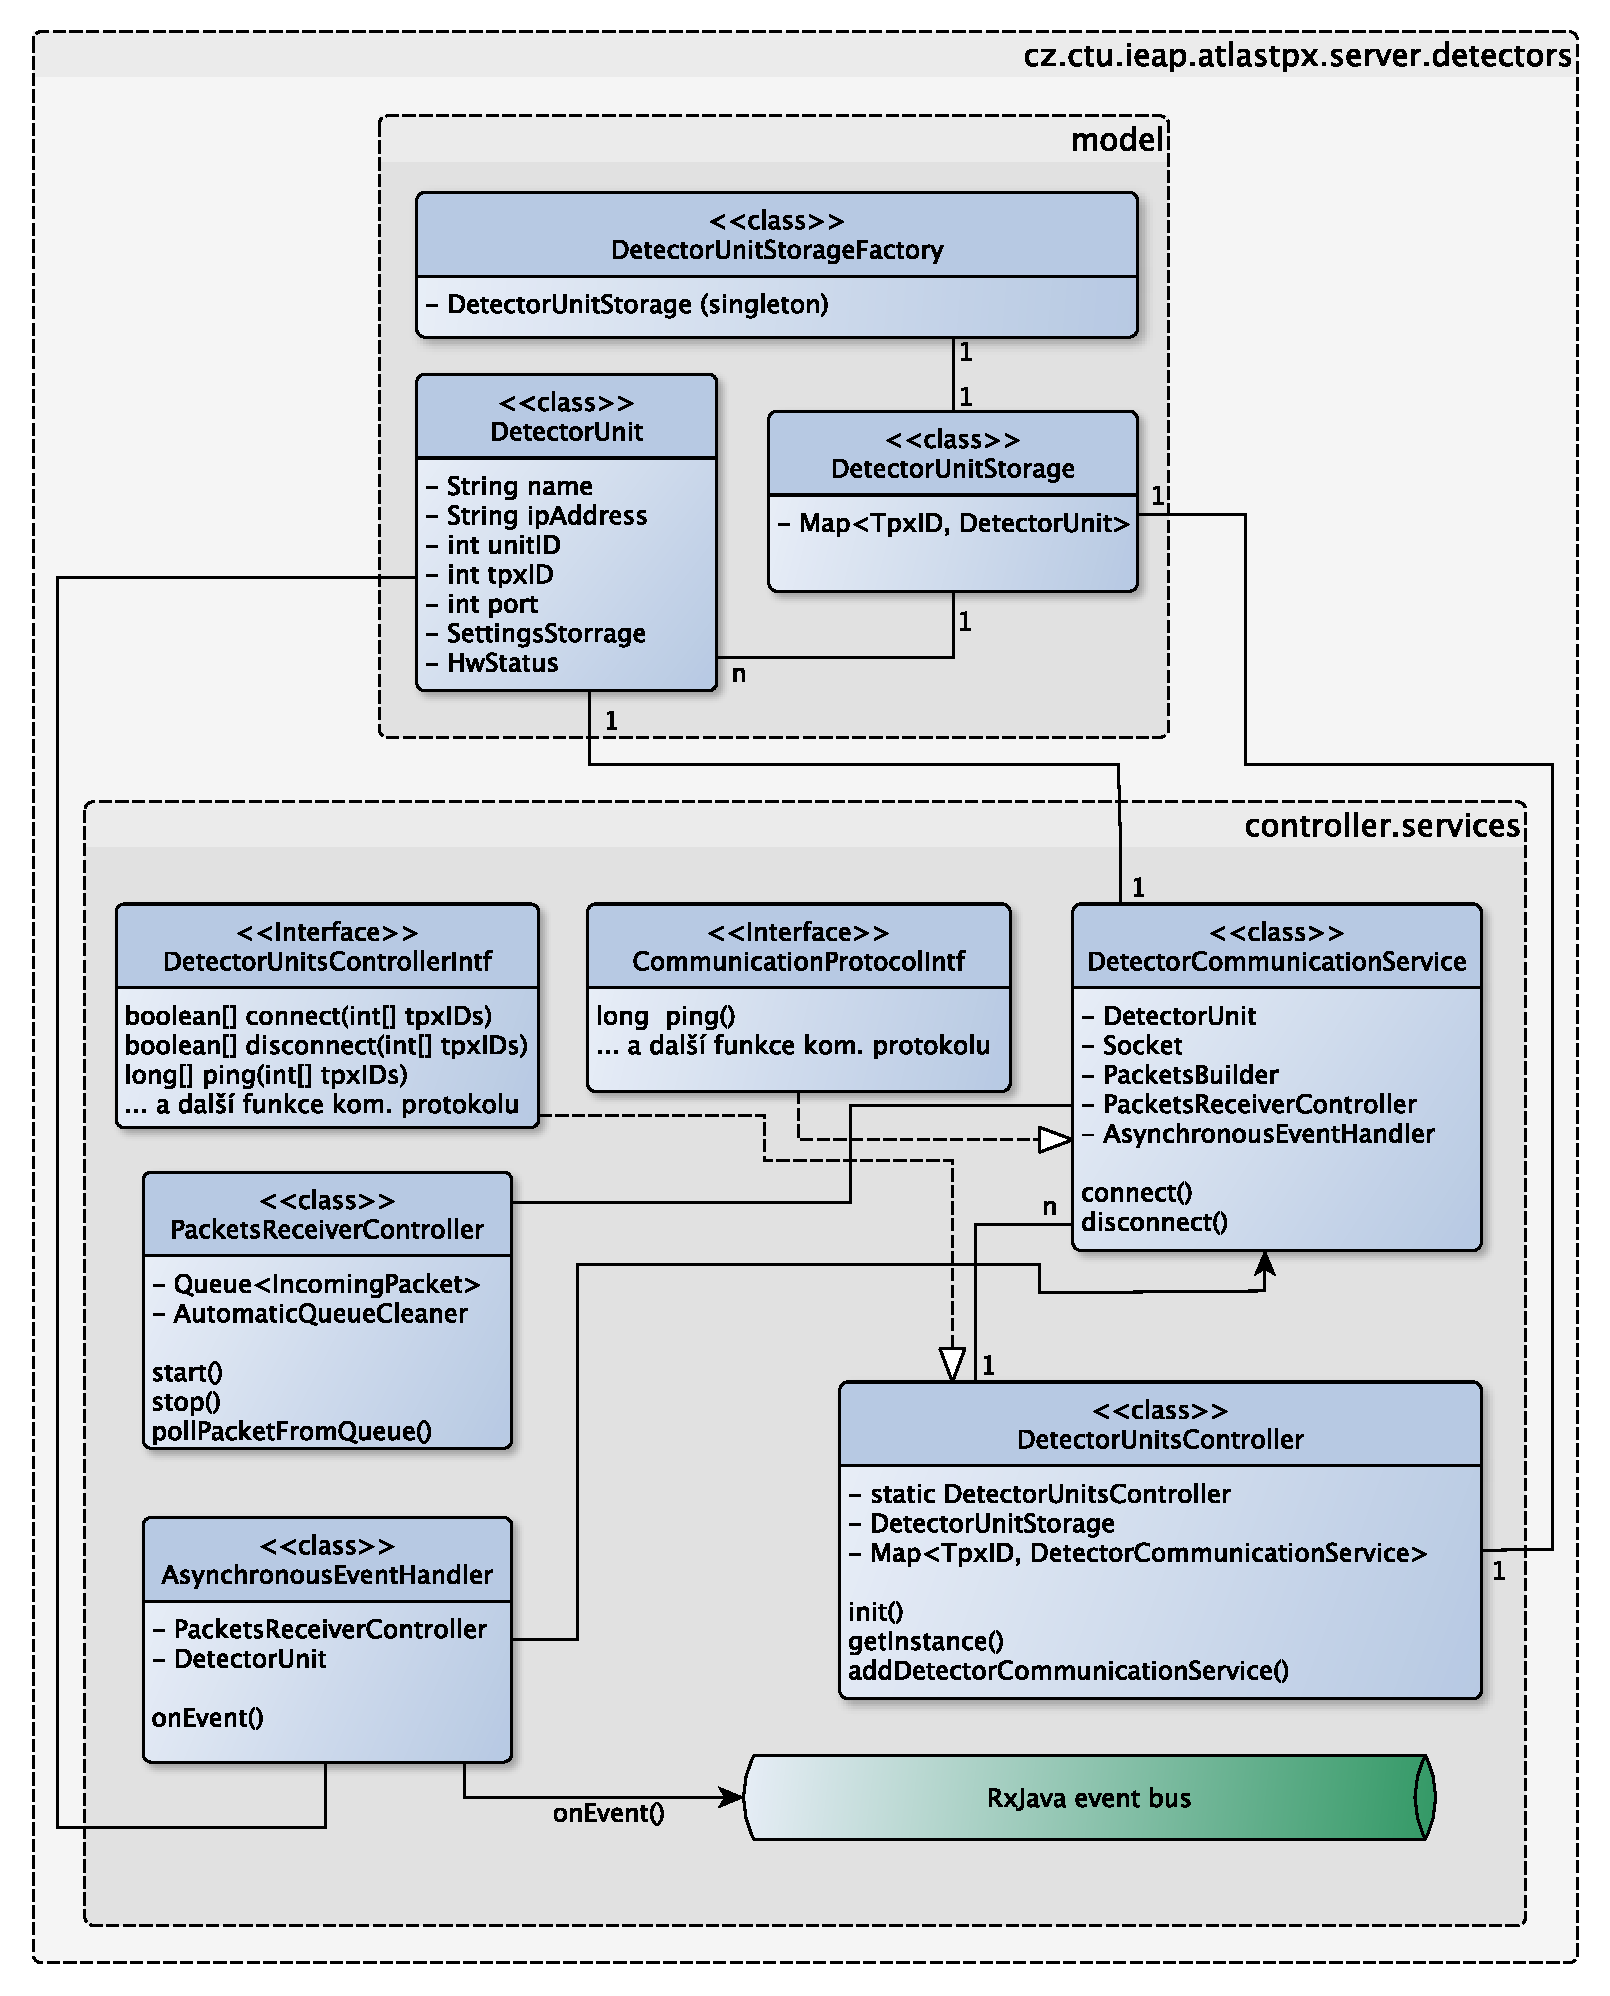
\includegraphics[width=11cm]{figures/atlas_tpx_detectors_class.pdf}
		\caption{Diagram tříd modulu pro ovládání detektorů}
		\label{fig:class:detectors}
	\end{center}
\end{figure}

Na obrázku \ref{fig:class:detectors} můžete vidět diagram tříd modulu pro práci s detektory řídícího softwaru. Tento diagram není úplný a obsahuje jen několik nejdůležitějších tříd, zbytek je k nalezení na přiloženém CD.

Při návrhu tohoto modulu bylo vycházeno z návrhového vzoru Model-View-Controller \cite{DesignPatterns-Gamma:1995:DPE:186897}, resp. z jeho modifikace Model-Controller, protože tento modul žádnou prezentační vrstvu nemá. 

Začněme popisem balíčku \texttt{model}. Jeho nejdůležitější třídou je třída \texttt{DetectorUnit}, která uchovává všechny informace o jednom detektoru, jako na příklad název, tpxID, unitID, ip adresu, port, \texttt{SettingsStorage} (úložiště nastavení detektoru, jako na příklad bias, clock, parametry akvizice, DAC hodnoty atd.) a \texttt{HwStatus} (tento objekt nese informace o posledních naměřeních údajích získaných z detektoru, jako třeba aktuální hodnoty bias, ping, obecný a měřící status apod.).

Pro uchovávání všech instancí třídy \texttt{DetectorUnit} slouží singleton \cite{DesignPatterns-Gamma:1995:DPE:186897} třída \texttt{DetectorUnit\\Storage}, která tyto instance uchovává v kolekci HashMap, jejímž klíčem je TpxID (Integer). Instanci tohoto singletonu je možné získat pomocí třídy \texttt{DetectorUnitStorageFactory}, resp. pomocí její statické metody \texttt{getStorage()}. Před prvním použití je třeba nejprve toto úložiště inicializovat pomocí statické metody \texttt{DetectorUnitStorageFactory.initStorage(String\\initFilePath)}, které se coby parametr předá cesta v souborovém systému k "*.csv" souboru s tabulkou s detektory. Každý řádek tohoto souboru reprezentuje jeden detektor a je v následujícím formátu:
\begin{center}
	název\_detektoru\textbf{\Large{;}}ip\_adresa\textbf{\Large{;}}unit\_id\textbf{\Large{;}}tpx\_id\textbf{\Large{;}}port
\end{center}

V balíčku \texttt{controller.services} se nachází vlastní logika tohoto modulu. 
Třída \texttt{Detector\\CommunicationService} se stará o vlastní komunikaci s detektorem (jedna instance = jeden detektor). Tato třída obsahuje instanci třídy \texttt{DetectorUnit} (předané v konstruktoru), která mimo jiné obsahuje IP adresu a port příslušného detektoru. Tyto parametry se používají v metodě \texttt{connect()}, ve které se vytvoří spojení s detektorem (socket, BufferedOutputStream, BufferedInputStream apod.). Pro odpojení detektoru zase slouží metoda \texttt{dicconnect()}. Krom metod pro síťovou komunikaci obsahuje i všechny metody implementované z interface \texttt{CommunicationProtocolIntf} - všechny synchronní metody komunikačního protokolu. 

Pro příjem příchozích paketů z detektoru vznikl \texttt{PacketsReceiverController}. Ten ve vlastním vlákně vyčítá proud bytů, přicházejících z detektoru a následně provádí jejich parsování, jehož výsledkem je instance objektu \texttt{IncomingPacket}, které obsahuje typ příkazu, příznak chyby a vlastní data. Takto vzniklý paket je zařazen do fronty příchozích paketů detektoru (implementované jako \texttt{ConcurrentLinkedQueue<IncomingPacket>}). Nad touto frontou pracují jednak všechny metody se synchronními příkazy komunikačního protokolu (které sledují, zda-li se v ní v daném časovém intervalu objeví odpověď), ale také instance objetu \texttt{AsynchronousEventHandlerController}. Ten ve vlastním vlákně tuto frontu sleduje a objeví-li se paket s typem příkazu \texttt{0xFD (Asynchronous Event From Device)}, tak ho z fronty odebere, jeho vlastní data rozparsuje a dále zpracuje. Pokud se na příklad jedná o událost dokončené akvizice, tak \texttt{ReadOutService} snímek z detektoru vyčte a pomocí \texttt{RxJava event bus} vyšle asynchronní zprávu napříč celou aplikací s vyčteným snímkem. Zde byl použit návrhový vzor Producer - Consumer, kde \texttt{AsynchronousEventHandlerController} představuje Producer a na kterémkoliv jiném místě aplikace se Consumer (možno i více Consumerů) muže zaregistrovat ke sledování událostí v event bus. Příkladem takového Comsumera může být \texttt{FrameSaverController}, který se postará o uložení získaného snímku (viz kapitola \ref{atlas:cont:output}).

Aby bylo možné pohodlně ovládat více detektorů současně, vznikl\\\texttt{DetectorUnitsController}. Ten implementuje interface \texttt{DetectorUnitsControllerIntf}, jehož metody pokrývají veškerou funkcionalitu detektoru, jako třeba metody k navázání a ukončení spojení, ale také všechny metody komunikačního protokolu. Všechny tyto metody mají jeden společní parametr - \texttt{int[] tpxIDs} (pole TpxID detektorů). Tento parametr určuje, nad kterými detektory se má daná metoda hromadně vykonat. Jejich výstupem je zase pole, jehož typ se liší dle příkazu (na příklad pro metodu connect je to pole boolean proměnných - značící úspěch připojení, pro ping zase double čísel, udávajících odezvu spojení v $ns$). Tento objekt je zase typu singleton a jeho instanci lze získat pomocí metody \texttt{getInstance()}. Po spuštění aplikace je však třeba tento singleton nainicializovat pomocí metody \texttt{init()}, která pomocí \texttt{DetectorUnitStorageFactory} vytvoří datovou strukturu  s \texttt{DetectorCommunicationService} jednotlivých detektorů.


%********************************************************************************
% Řídící software a jeho implementace - Řízení detektorů
% > Emulátor detektoru
%********************************************************************************
\subsubsection{Emulátor detektoru}
Pro účely vývoje a testování řídícího software pro \texttt{Atlas TPX server} byl vyvinut emulátor detektoru, který plně emuluje jeho činnost. Emulátor byl rovněž napsán v jazyce \texttt{JAVA} a jeho zdrojové kódy a spustitelný \texttt{jar} soubor naleznete na přiloženém CD.

Emulátor se spouští se dvěma povinnými parametry, kde
\begin{enumerate}
	\item je port, na kterém server emulátoru naslouchá (celé číslo),
	\item je pravděpodobnost, s jakou při zpracovávání požadavku bude simulována chyba - $0$ znamená bez chyb, $1$ samé chyby (desetinné číslo).
\end{enumerate}

\begin{figure}[t]
	\begin{center}
		\begin{sequencediagram}
			\newinst{ss}{:AtlasPix (ServerSocket)}
			\newthread[blue]{ch}{:ClientHandler}
			\newthread[gray]{pr}{:PaketReceiver}
			\newthread[red]{ap}{:AcquisitionPerformer}
			\begin{sdblock}{Připojení klienta}{}
				\begin{call}{ss}{acceptClient}{ch}{success}
					\begin{call}{ch}{startReceiving}{pr}{success}
					\end{call}
				\end{call}
			\end{sdblock}
			\begin{sdblock}{Akvizice snímku}{}
				\begin{callself}{pr}{performAcqRequest}{success}
					\begin{call}{pr}{acqRequest}{ch}{success}
						\mess{ch}{performAcq}{ap}
					\end{call}	
				\end{callself}	
				\postlevel
				\mess{ap}{onAcqPerformed}{ch}
				\begin{callself}{ch}{onAcqPerformed}{success}
				\end{callself}	
			\end{sdblock}			
		\end{sequencediagram}
		\caption{Emulátor detektoru - sekvenční diagram připojení klienta a pořízení snímku}
		\label{fig:uml:emulator}
	\end{center}
\end{figure}

Na obrázku \ref{fig:uml:emulator} je zobrazen sekvenční diagram dvou případů užití tohoto emulátoru. První případ užití znázorňuje připojení klienta (na př. \texttt{Atlas TPX serveru}) a druhý pak proces zpracování žádosti o snímek a jeho vygenerování.

Pojďme si nyní popsat první část - připojení klienta. Ve třídě \texttt{AtlasPix}, resp. v její metodě \texttt{startServer()} se nachází nekonečná smyčka, ve které je pomocí instance třídy \texttt{ServerSocket} navázáno spojení s novými klienty. Když spojení s klientem je navázáno, je vytvořen klientský socket, pomocí kterého dojde v vytvoření instance třídy \texttt{ClientHandler}. Ta se v samostatném novém vláknu stará o obsluhu nově připojeného klienta. Zároveň \texttt{ClientHandler} vytvoří instanci třídy \texttt{PaketReceiver}, který čte proud bytů přijatých od klienta a parsuje jej do objektů typu \texttt{IncomingPacket}.

Tím se dostáváme k druhému příkladu případu užití - akvizici snímku. Poté, co \texttt{PaketReceiver} přijme nový paket, tak ho vloží do fronty paketů. Tuto frontu z druhé strany čte a zpracovává \texttt{ClientHandler}. Všechny příchozí pakety od klienta mohou obsahovat jen synchronní příkazy komunikačního protokolu, takže může být okamžitě nasimulován příslušný stav emulátoru a vygenerována odpověď klientovi. 

V našem případe akvizice snímku je situace trochu složitější. \texttt{PaketReceiver} odchytí nový paket, obsahující žádost o provedení akvizice, který předá do fronty příchozích paketů. Když se \texttt{ClientHandler} dostane k jeho zpracování, tak vytvoří objekt typu \texttt{AcquisitionRequest} a předá ho instanci třídy \texttt{AcquisitionPerformer}. Ten žádost o akvizici zařadí do příslušní fronty, kde čeká, až samostatné akviziční vlákno se dostane k jejímu zpracování. Při zpracovávání žádosti o akvizici je vygenerováno náhodná matice hodnot pixelů (o velikosti $256\times512$) a také příslušná metadata, jako na příklad akviziční čas, bias obou čipů (s přičtenou náhodnou veličinou, simulující fluktuaci napětí na křemíkovém povrchu detekčních čipů) apod. Po vygenerování těchto hodnot se akviziční vlákno uspí na dobu akvizice, aby se chování emulátoru co nejvíce přiblížilo skutečnému detektoru.

Následně je připojenému klientovi poslána asynchronní zpráva o dokončené akvizici. Tato zpráva obsahuje příznak, že naměřená data jsou připravena k vyčtení a také ID vygenerovaného snímku. 

Poté klient pošle příkaz pro vyčtení naměřených dat (resp. dva příkazy - jeden pro vlastní snímek a druhý pro metadata), což bylo popsáno v kapitole \ref{atlas:com:synchonni_a_asynchonni_prikazy} - viz obr. \ref{fig:uml:com_priklad}.

%********************************************************************************
% Řídící software a jeho implementace - REST API server
%********************************************************************************
\subsection{REST API server}\label{atlas:cont:api}
Řídící software se svému ovládání poskytuje rozhraní přes \texttt{JSON REST\footnote{z angl. Representational State Transfer} API}. Pro toto rozhraní byla použita knihovna Dropwizard\cite{dropwizard}, která vznikla složením několika dalších knihoven, zejména pak:
\begin{description}
	\item[Jetty] je open-source software, v současné době vyvíjen Eclipse Foundation. Tato knihovna obsahuje Java HTTP webový server, který na rozdíl od běžných webových serveru (které vetšinou přes HTTP protokol poskytují soubory koncovým uživatelům) byl navržen pro strojově orientovanou komunikaci.
	\item[Jersey] je open-source knihovna (která dle \cite{dropwizard} vychází z \texttt{JAX-RS}\footnote{\url{http://jcp.org/en/jsr/detail?id=311}}) a byla použita pro zajištění REST API. Tato knihovna umožňuje elegantně pomocí anotací mapovat HTTP dotazy na jednoduché Java objety.
	\item[Jackson] je výkonný nástroj pro práci s \texttt{JSON}\footnote{JSON je v dnešní době standardem pro zápis a výměnu strukturovaných, člověkem i strojem čitelných dat.} objekty v jazyce Java. Tato knihovna umožňuje ergonomicky mapovat data v JSON do Java objektů pomocí anotací.
\end{description}

V této podkapitole bude popsána implementace této knihovny do \texttt{Atlas TPX serveru} a její provázanost na modul pro řízení detektorů (\ref{atlas:cont:impl}).

%********************************************************************************
% Řídící software a jeho implementace - REST API server
% > Konfigurace a spuštění serveru
%********************************************************************************
\subsubsection{Konfigurace a spuštění serveru}
Server je možné spustit z příkazové řádky pomocí příkazu \texttt{"java -jar atlasTpxServer.jar server config.yml"}, kde \texttt{atlasTpxServer.jar} je spustitelný binární soubor serveru, \texttt{server} je povinný parametr (znamenající spuštění programu v módu server) a \texttt{config.yml}, což je také povinný parametr, udávající cestu v souborovém systému ke konfiguračnímu souboru serveru.

V příloze \ref{app:config} strukturu tohoto konfiguračního souboru, ve kterém je možné nastavit následující:
\begin{description}
	\item[Umístění tabulky s detektory] (detectorsConfigPath - viz \ref{app:config} řádek 8)\\
		Tento parametr udává cestu v souborovém systému ke konfiguračnímu "*.csv" souboru, obsahující tabulku všech detektoru a jejich parametrů, popsanou v \ref{atlas:cont:impl}.
	\item[Nastavení webového serveru] (server - viz \ref{app:config} řádek 11)\\
		V rámci tohoto objektu je možné nastavit použitý typ protokolu spojení (\texttt{HTTP}/\texttt{HTTPS}), port, počty vláken a další.
	\item[Logování] (logging - viz \ref{app:config} řádek 30)\\
		Pomocí tohoto parametru je možné nastavit úroveň a cíl vytvářených logů. V přiloženém konfiguračním souboru bylo použito dvojího logování a to na standardní výstup a do souboru (oba úrovně \texttt{INFO}). Při logování do souboru je možné navíc nastavit automatickou archivaci.
	\item[Automatické vyčítání snímků] (readOutDataAutomatically - viz \ref{app:config} řádek 54)\\
		Tento parametr typu \texttt{boolean} udává, když přijde asynchronní událost z detektoru o datech připravených k vyčtení, zda-li budou vyčtena automaticky (při hodnotě parametru \texttt{true}), nebo manuálně (při hodnotě \texttt{false}).
	\item[Výstupní adresář] (outputDir - viz \ref{app:config} řádek 57)\\
		Parametr udávající cestu v souborovém systému pro ukládání dat z detektorů.
	\item[Formát výstupních dat] (outputFramesType - viz \ref{app:config} řádek 68)\\
		Tento parametr obsahuje pole výstupních formátu dat, ve kterých získaná data z detektorů budou ukládána. V této verzi programu je podporovaný jediný formát - \texttt{MULTIFRAME}.
	\item[Konfigurace data serveru] (v \ref{app:config} od řádku 77)\\
		Na tomto místě je možné nastavit parametry (url a port) serveru, sloužícího pro příjem a zpracování naměřených dat a zda-li má být použit. Více o tomto serveru bude zmíněno v \ref{atlas:cont:output:dataserver}.
\end{description}

%********************************************************************************
% Řídící software a jeho implementace - REST API server
% > Metody poskytované serverem
%********************************************************************************
\subsubsection{Metody poskytované serverem}


\clearpage
%********************************************************************************
% Řídící software a jeho implementace - REST API server
% > Výkonost
%********************************************************************************
\subsubsection{Výkonost}


\clearpage
\subsection{Zpracování a ukládání dat}\label{atlas:cont:output}
\subsubsection{Data server}\label{atlas:cont:output:dataserver}










\addbibresource{reference.bib}

\chapter{Závěr}
Jedním z~cílů této bakalářské práce bylo vyvinutí software pro řízení sítě hybridních částicových pixelových detektorů (označované jako \texttt{ATLAS TPX}), operujících uvnitř ATLAS experimentu na LHC v~CERN - viz kapitola \ref{calib}. v~rámci této práce byl navržen a~implementován software, který pomocí multi-vláknového přístupu umožňuje současně ovládat všechny detektory této sítě, zejména pak řízení akvizice dat, vyčítání pořízených snímků, nastavování měřících parametrů a~také vyčítání a~uchovávání stavových informací detektorů. Řídící software rovněž poskytuje \texttt{JSON REST API} server pro své vzdálené ovládání, díky kterému bude mino jiné možné řízení této detektorové sítě implementovat do CERNského systému pro řízení a~kontrolu detektorů (tzv. \texttt{DCS}). Další implementovanou funkcionalitou tohoto software je zpracování a~ukládání pořízených dat z~detektorů - ty mohou být ukládány v~\texttt{Multiframe} formátu do předem definovaného úložiště nebo odesílány datovému serveru pomocí jeho \texttt{API}, které data dále zpracuje a~uloží do CERNského systému pro skladování dat (\texttt{EOS}).

Dalším cílem této práce bylo vyvinutí nástrojů pro energetickou kalibrací sítě \texttt{ATLAS TPX}, pomocí metody popsané v~\cite{Jakubek2011S262}. Byl vyvinut univerzální software \ref{calib:sw}, který uživateli umožňuje průchod procesem zpracování dat pro energetickou kalibraci libovolného detektoru, pracujícího v~\texttt{Time-Over-Treshold} módu. v~rámci kalibračního procesu software ze spekter jednotlivých pixelů a~pro různé zdroje záření vytvoří jednotlivé kalibrační body, ze kterých pak sestaví kalibrační funkci (viz vzorec \ref{eq:calib:calib_function}), udávající vztah mezi energií a~TOT, pro každý pixel detektoru. Software rovněž nabízí nástroje pro ověření kvality vstupních dat, kvality detektoru, ověření kvality kalibrace a~také pro různé dodatečné úpravy výstupu kalibračního procesu, popsané v~\ref{calib:sw:post_process}.

V této práci byly rovněž shrnuty a~popsány vlastnosti hybridních částicových pixelových detektorů rodiny Medipix - viz kapitola \ref{det}.

%\chapter{Úvod}
Výsledná struktura vaší práce a názvy a rozsahy jednotlivých kapitol se samozřejmě budou lišit podle typu práce a podle konkrétní povahy zpracovávaného tématu. 

\section{Jak používat tuto šablonu}

\chapter{Pokyny a návody k formátování textu práce}
Používat se dají všechny příkazy systému \LaTeX. Existuje velké množství volně přístupné dokumentace, tutoriálů, příruček a dalších materiálů v elektronické podobě. Výchozím bodem, kromě Googlu, může být stránka CSTUG (Czech Tech Users Group) \cite{CSTUG}. Tam najdete odkazy na další materiály.  Vetšinou dostačující a přehledně organizovanou elektronikou dokumentaci najdete například na \cite{latexdocweb} nebo \cite{latexwiki}.

Existují i různé nadstavby nad systémy \TeX{} a \LaTeX, které výrazně usnadní psaní textu zejména začátečníkům. Z mnoha možných uvádíme: Kile\footnote{\url{http://kile.sourceforge.net/}}, TexMaker\footnote{\url{http://www.xm1math.net/texmaker/}}, LyX\footnote{\url{http://www.lyx.org/}}.


%%%%%%%%%%%%%%%%%%%%%%%%%% 
% Pro snadnejsi praci s vetsimi texty je rozumne tyto rozdelit
% do samostatnych souboru nejlepe dle kapitol a tyto potom vkladat
% pomoci prikazu \include{jmeno_souboru}.
% Napr.:
% \include{1_uvod}
% \include{2_teorie}
% atd...
%%%%%%%%%%%%%%%%%%%%%%%%%% 



\section{Tabulky}
Existuje více způsobů, jak sázet tabulky. Například je možno použít prostředí \verb|table|, které je velmi podobné prostředí \verb|figure|. 

\begin{table}
\begin{center}
\begin{tabular}{|c|l|l|}
\hline
\textbf{DTD} & \textbf{construction} & \textbf{elimination} \\
\hline
$\mid$ & \verb+in1|A|B a:sum A B+ & \verb+case([_:A]a)([_:B]a)ab:A+\\
&\verb+in1|A|B b:sum A B+ & \verb+case([_:A]b)([_:B]b)ba:B+\\
\hline
$+$&\verb+do_reg:A -> reg A+&\verb+undo_reg:reg A -> A+\\
\hline
$*,?$& the same like $\mid$ and $+$ & the same like $\mid$ and $+$\\
& with \verb+emtpy_el:empty+ & with \verb+emtpy_el:empty+\\
\hline
R(a,b) & \verb+make_R:A->B->R+ & \verb+a: R -> A+\\
 & & \verb+b: R -> B+\\
\hline
\end{tabular}
\end{center}
\caption{Ukázka tabulky}
\label{tab:tab1}
\end{table}

Zdrojový text tabulky \ref{tab:tab1} vypadá takto:
\begin{verbatim}
\begin{table}
\begin{center}
\begin{tabular}{|c|l|l|}
\hline
\textbf{DTD} & \textbf{construction} & \textbf{elimination} \\
\hline
$\mid$ & \verb+in1|A|B a:sum A B+ & \verb+case([_:A]a)([_:B]a)ab:A+\\
&\verb+in1|A|B b:sum A B+ & \verb+case([_:A]b)([_:B]b)ba:B+\\
\hline
$+$&\verb+do_reg:A -> reg A+&\verb+undo_reg:reg A -> A+\\
\hline
$*,?$& the same like $\mid$ and $+$ & the same like $\mid$ and $+$\\
& with \verb+emtpy_el:empty+ & with \verb+emtpy_el:empty+\\
\hline
R(a,b) & \verb+make_R:A->B->R+ & \verb+a: R -> A+\\
 & & \verb+b: R -> B+\\
\hline
\end{tabular}
\end{center}
\caption{Ukázka tabulky}
\label{tab:tab1}
\end{table}
\begin{table}
\end{verbatim}

A pokud máte svá data v CSV můžete použít některou z knihoven nabízených v   http://texblog.org/2012/05/30/generate-latex-tables-from-csv-files-excel/ 

\section{Odkazy v textu}
\subsection{Odkazy na literaturu}
Jsou realizovány příkazem \verb|\cite{odkaz}|. 

Seznam literatury je dobré zapsat do samostatného souboru a ten pak zpracovat programem bibtex (viz soubor \verb|reference.bib|). Zdrojový soubor pro \verb|bibtex| vypadá například takto:
\begin{verbatim}
@Article{Chen01,
  author  = "Yong-Sheng Chen and Yi-Ping Hung and Chiou-Shann Fuh",
  title   = "Fast Block Matching Algorithm Based on 
             the Winner-Update Strategy",
  journal = "IEEE Transactions On Image Processing",
  pages   = "1212--1222",
  volume  =  10,
  number  =   8,
  year    = 2001,
}

@Misc{latexdocweb,
  author  = "",
  title   = "{\LaTeX} --- online manuál",
  note    = "\verb|http://www.cstug.cz/latex/lm/frames.html|",
  year    = "",
}
...
\end{verbatim}

%11.12.2008, 3.5.2009
\textbf{Pozor:} Sazba názvů odkazů je dána Bib\TeX{} stylem\\ (\verb|\bibliographystyle{abbrv}|). 
%Budete-li používat české prostředí (\verb|\usepackage[czech]{babel}|), 
Bib\TeX{} tedy obvykle vysází velké pouze počáteční písmeno z názvu zdroje, 
ostatní písmena zůstanou malá bez ohledu na to, jak je napíšete. 
Přesněji řečeno, styl může zvolit pro každý typ publikace jiné konverze. 
Pro časopisecké články třeba výše uvedené, jiné pro monografie (u nich často bývá 
naopak velikost písmen zachována).

Pokud chcete Bib\TeX u napovědět, která písmena nechat bez konverzí 
(viz \texttt{title = "\{$\backslash$LaTeX\} -{}-{}- online manuál"} 
v~předchozím příkladu), je nutné příslušné písmeno (zde celé makro) uzavřít 
do složených závorek. Pro přehlednost je proto vhodné celé parametry 
uzavírat do uvozovek (\texttt{author = "\dots"}), nikoliv do složených závorek.

Odkazy na literaturu ve zdrojovém textu se pak zapisují:
\begin{verbatim}
Podívejte se na \cite{Chen01}, 
další detaily najdete na \cite{latexdocweb}
\end{verbatim}

Vazbu mezi soubory \verb|*.tex| a \verb|*.bib| zajistíte příkazem 
\verb|\bibliography{}| v souboru \verb|*.tex|.  V našem případě tedy zdrojový 
dokument \verb|thesis.tex| obsahuje příkaz\\
\verb|\bibliography{reference}|.

Zpracování zdrojového textu s odkazy se provede postupným voláním programů\\
\verb|pdflatex <soubor>| (případně \verb|latex <soubor>|), \verb|bibtex <soubor>| 
a opět\\ \verb|pdflatex <soubor>|.\footnote{První volání \texttt{pdflatex} 
vytvoří soubor s~koncovkou \texttt{*.aux}, který je vstupem pro program 
\texttt{bibtex}, pak je potřeba znovu zavolat program \texttt{pdflatex} 
(\texttt{latex}), který tentokrát zpracuje soubory s příponami \texttt{.aux} a 
\texttt{.tex}. 
Informaci o případných nevyřešených odkazech (cross-reference) vidíte přímo při 
zpracovávání zdrojového souboru příkazem \texttt{pdflatex}. Program \texttt{pdflatex} 
(\texttt{latex}) lze volat vícekrát, pokud stále vidíte nevyřešené závislosti.}


Níže uvedený příklad je převzat z dříve existujících pokynů studentům, kteří 
dělají svou diplomovou nebo bakalářskou práci v~Grafické skupině.\footnote{Několikrát 
jsem byl upozorněn, že web s těmito pokyny byl zrušen, proto jej zde přímo necituji. 
Nicméně příklad sám o sobě dokumentuje obecně přijímaný konsensus ohledně citací 
v~bakalářských a diplomových pracích na KP.} Zde se praví:
\begin{small}
\begin{verbatim}
...
j) Seznam literatury a dalších použitých pramenů, odkazy na WWW stránky, ...
 Pozor na to, že na veškeré uvedené prameny se musíte v textu práce 
 odkazovat -- [1]. 
Pramen, na který neodkazujete, vypadá, že jste ho vlastně nepotřebovali 
a je uveden jen do počtu. Příklad citace knihy [1], článku v časopise [2], 
stati ve sborníku [3] a html odkazu [4]: 
[1] J. Žára, B. Beneš;, and P. Felkel. 
     Moderní počítačová grafika. Computer Press s.r.o, Brno, 1 edition, 1998. 
     (in Czech). 
[2] P. Slavík. Grammars and Rewriting Systems as Models for Graphical User 
     Interfaces. Cognitive Systems, 4(4--3):381--399, 1997. 
[3] M. Haindl, Š. Kment, and P. Slavík. Virtual Information Systems. 
     In WSCG'2000 -- Short communication papers, pages 22--27, Pilsen, 2000. 
     University of West Bohemia. 
[4] Knihovna grafické skupiny katedry počítačů: 
     http://www.cgg.cvut.cz/Bib/library/ 
\end{verbatim}
\end{small}
\ldots{} abychom výše citované odkazy skutečně našli v (automaticky generovaném) seznamu literatury tohoto textu, musíme je nyní alespoň jednou citovat: Kniha \cite{kniha}, článek v~časopisu \cite{clanek}, příspěvek na konferenci \cite{sbornik}, www odkaz \cite{www}.

Ještě přidáme další ukázku citací online zdrojů podle české normy. Odkaz na wiki o frameworcich \cite{wiki:framework} a ORM \cite{wiki:orm}. Použití viz soubor \verb|reference.bib|. V seznamu literatury by nyní měly být živé odkazy na zdroje. V \verb|reference.bib| je zcela nový typ publikace. Detaily dohledal a dodal Petr Dlouhý v dubnu 2010. Podrobnosti najdete ve zdrojovém souboru tohoto textu v komentáři u příkazu \verb|\thebibliography|.

\subsection{Odkazy na obrázky, tabulky a kapitoly}
\begin{itemize}
\item Označení místa v textu, na které chcete později čtenáře práce odkázat, se provede příkazem \verb|\label{navesti}|. Lze použít v prostředích \verb|figure| a  \verb|table|, ale též za názvem kapitoly nebo podkapitoly.
\item Na návěští se odkážeme příkazem \verb|\ref{navesti}| nebo \verb|\pageref{navesti}|.
\end{itemize}

\section{Rovnice, centrovaná, číslovaná matematika}
Jednoduchý matematický výraz zapsaný přímo do textu se vysází pomocí prostředí \verb|math|, resp. zkrácený zápis pomocí uzavření textu rovnice mezi znaky \verb|$|.

Kód \verb|$ S = \pi * r^2 $| bude vysázen takto: $ S = \pi * r^2 $.

Pokud chcete nečíslované rovnice, ale umístěné centrovaně na samostatné řádky, pak lze použít prostředí \verb|displaymath|, resp. zkrácený zápis pomocí uzavření textu rovnice mezi znaky \verb|$$|. Zdrojový kód: 
\begin{verb}
|$$ S = \pi * r^2 $$|
\end{verb}
bude pak vysázen takto:
$$ S = \pi * r^2 $$

Chcete-li mít rovnice číslované, je třeba použít prostředí \verb|eqation|. Kód:
\begin{verbatim}
\begin{equation}
  S = \pi * r^2
\end{equation}

\begin{equation}
  V = \pi * r^3
\end{equation}
\end{verbatim}
je potom vysázen takto:
\begin{equation}
  S = \pi * r^2
\end{equation}

\begin{equation}
  V = \pi * r^3
\end{equation}

\section{Kódy a algoritmy}
\subsection{Zdrojové kódy}
Chceme-li vysázet například část zdrojového kódu programu, hodí se prostředí \verb|verbatim|, které je bez formátování: 
\begin{verbatim}
         (* nickname2 *)
Lego> Refine in1
             (do_reg (nickname1 h));
Refine by  in1 (do_reg (nickname1 h))
   ?4 : pcdata
   ?5 : pcdata
          (* surname2 *)
Lego> Refine surname1 h;
Refine by  surname1 h
   ?5 : pcdata
          (* email2 *)
Lego> Refine undo_reg (email1 h);
Refine by  undo_reg (email1 h)
*** QED ***
\end{verbatim}

nebo se dá použít \verb|listings|, což je package, který umožňuje i syntax higlighting podle jazyka:

\lstset{language=Python} %následuje python kód a použije se python syntax
\begin{lstlisting}
	print 'Hello, world!'
\end{lstlisting}

a umožňuje načíst i přiložené zdrojové soubory:

%\lstinputlisting[language=C]{code/hello.c}

\subsection{Algoritmy}
Pokud chcete v práci popsat obecné algoritmy s využitím pseudokódu, můžete použít knihovny \verb|algorithmicx| a \verb|algpseudocode|:
\begin{algorithmic}
\If {$i\geq maxval$}
    \State $i\gets 0$
\Else
    \If {$i+k\leq maxval$}
        \State $i\gets i+k$
    \EndIf
\EndIf
\end{algorithmic}

\section{Zkratky}
V tomto textu používám několik zkratek, třeba 2D\nomenclature{2D}{Two-Dimensional} nebo \nomExpl{KNB}{Killing nanobots}. V úvodní části dokumentu můžete nastavit/upravit příkaz pro zadání zkratky, pokud např. chcete mít význam zkratky pod čarou. Všechny zkratky se vytisknou podle abecedy (\nom{ABC}{Zkratka pro abecedu}) v příloze \ref{apx:zkratky}, aby toto fungovalo musíte vybudovat index pomocí příkazu:
\begin{verbatim}
		makeindex soubor.nlo -s nomencl.ist -o soubor.nls
\end{verbatim}

\section{České uvozovky}
V souboru \verb|k336_thesis_macros.tex| je příkaz \verb|\uv{}| pro sázení českých uvozovek. \uv{Text uzavřený do českých uvozovek.}

\chapter{Závěr}

\begin{itemize}
\item Zhodnocení splnění cílů DP/BP a  vlastního přínosu práce (při formulaci je třeba vzít v potaz zadání práce).
\item Diskuse dalšího možného pokračování práce.
\end{itemize} 


%\section{Obrázky}
Obrázky jsou vhodným nástrojem pro ilustraci a doplnění textu, používejte je v rozumné míře ať vaše práce nepřipomíná komix. Při hledání/tvorbě obrázků nezapomeňte na to, že u přejatých obrázků musíte odkazovat jejich zdroj a že obrázky by měly být čitelné (typicky .jpg soubory se často rozostří). Dalším častým neduhem jsou obrázky s anglickými popisky v česky psaném textu, pokud to je možné udržte jazyk práce jednotný.

\subsection{Vkládání obrázků}
Obrázky se umísťují do plovoucího prostředí \verb|figure|. Každý obrázek by měl obsahovat \textbf{název} (\verb|\caption|) a \textbf{návěští} (\verb|\label|). Použití příkazu pro vložení obrázku \\\verb|\includegraphics| je podmíněno aktivací (načtením) balíku graphicx příkazem\\ \verb|\usepackage{graphicx}|.

Budete-li zdrojový text zpracovávat pomocí programu \verb|pdflatex|, očekávají se obrázky s příponou \verb|*.pdf|\footnote{pdflatex umí také formáty PNG a JPG.}, použijete-li k formátování \verb|latex|, očekávají se obrázky s příponou \verb|*.eps|.\footnote{Vzájemnou konverzi mezi snad všemi typy obrazku včetně změn vekostí a dalších vymožeností vám může zajistit balík ImageMagic  (http://www.imagemagick.org/script/index.php). Je dostupný pod Linuxem, Mac OS i MS Windows. Důležité jsou zejména příkazy convert a identify.}

\begin{figure}[ht]
\begin{center}
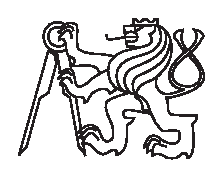
\includegraphics[width=5cm]{figures/LogoCVUT}
\caption{Popiska obrázku}
\label{fig:logo}
\end{center}
\end{figure}

Příklad vložení obrázku:
\begin{verbatim}
\begin{figure}[h]
\begin{center}
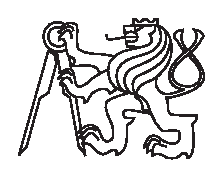
\includegraphics[width=5cm]{figures/LogoCVUT}
\caption{Popiska obrazku}
\label{fig:logo}
\end{center}
\end{figure}
\end{verbatim}

\subsection{Kreslení obrázků}
Zřejmě každý z vás má nějaký oblíbený nástroj pro tvorbu obrázků. Jde jen o to, abyste dokázali obrázek uložit v požadovaném formátu nebo jej do něj konvertovat (viz předchozí kapitola). Je zřejmě vhodné kreslit obrázky vektorově. Celkem oblíbený, na ovládání celkem jednoduchý a přitom dostatečně mocný je například program Inkscape.

Zde stojí za to upozornit na kreslící programe Ipe \cite{ipe}, který dokáže do obrázku vkládat komentáře přímo v latexovském formátu (vzroce, stejné fonty atd.). Podobné věci umí na Linuxové platformě nástroj Xfig. 

Za pozornost ještě stojí schopnost editoru Ipe importovat obrázek (jpg nebo bitmap) a krelit do něj latexovské popisky a komentáře. Výsledek pak umí exportovat přímo do pdf.

Další možností je knihovna graphviz, které vykreslí obrázek podle vašeho popisu (kódu), výstup je možný do mnoha formátů (.eps, .jpg, ...).


%%%%%%%%%%%%%%%%%%%%%%%%%% 
% Seznam literatury je v samostatnem souboru reference.bib. Ten
% upravte dle vlastnich potreb, potom zpracujte (a do textu
% zapracujte) pomoci prikazu bibtex a nasledne pdflatex (nebo
% latex). Druhy z nich alespon 2x, aby se poresily odkazy.

% originally following specification for bibliography formating was used
%\bibliographystyle{abbrv}

% Here is an improvment by Petr Dlouhy (April 2010).
% It is mainly for supervisors who expect Czech fomrating rules for references
% Additional feature is live url addresses to sources from your pdf file
% It requires the file csplainnat.bst (included in this sample zipfile).

\bibliographystyle{csplainnat}

%bibliographystyle{plain}
%\bibliographystyle{psc}
{
%JZ: 11.12.2008 Kdo chce mit v techto ukazkovych odkazech take odkaz na CSTeX:
\def\CS{$\cal C\kern-0.1667em\lower.5ex\hbox{$\cal S$}\kern-0.075em $}
\bibliography{reference}
}

% M. Dušek radi:
%\bibliographystyle{alpha}
% kdy citace ma tvar [AutorRok] (napriklad [Cook97]). Sice to asi neni  podle ceske normy (BTW BibTeX stejne neodpovida ceske norme), ale je to nejprehlednejsi.
% 3.5.2009 JZ polemizuje: BibTeX neobvinujte, napiste a poskytnete nam styl (.bst) splnujici citacni normu CSN/ISO.


%%%%%%%%%%%%%%%%%%%%%%%%%% 
% vše co následuje bude uvedeno v přílohách
\appendix	

\printnomenclature
\label{apx:zkratky}

\chapter{Obsah přiloženého CD}
\textbf{\large Tato příloha je povinná pro každou práci. Každá práce musí totiž obsahovat přiložené CD. Viz dále.}

Může vypadat například takto. Váš seznam samozřejmě bude odpovídat typu vaší práce... \cite{TurecekThesis2011} fasfassaafsaf

\begin{figure}[h]
\begin{center}
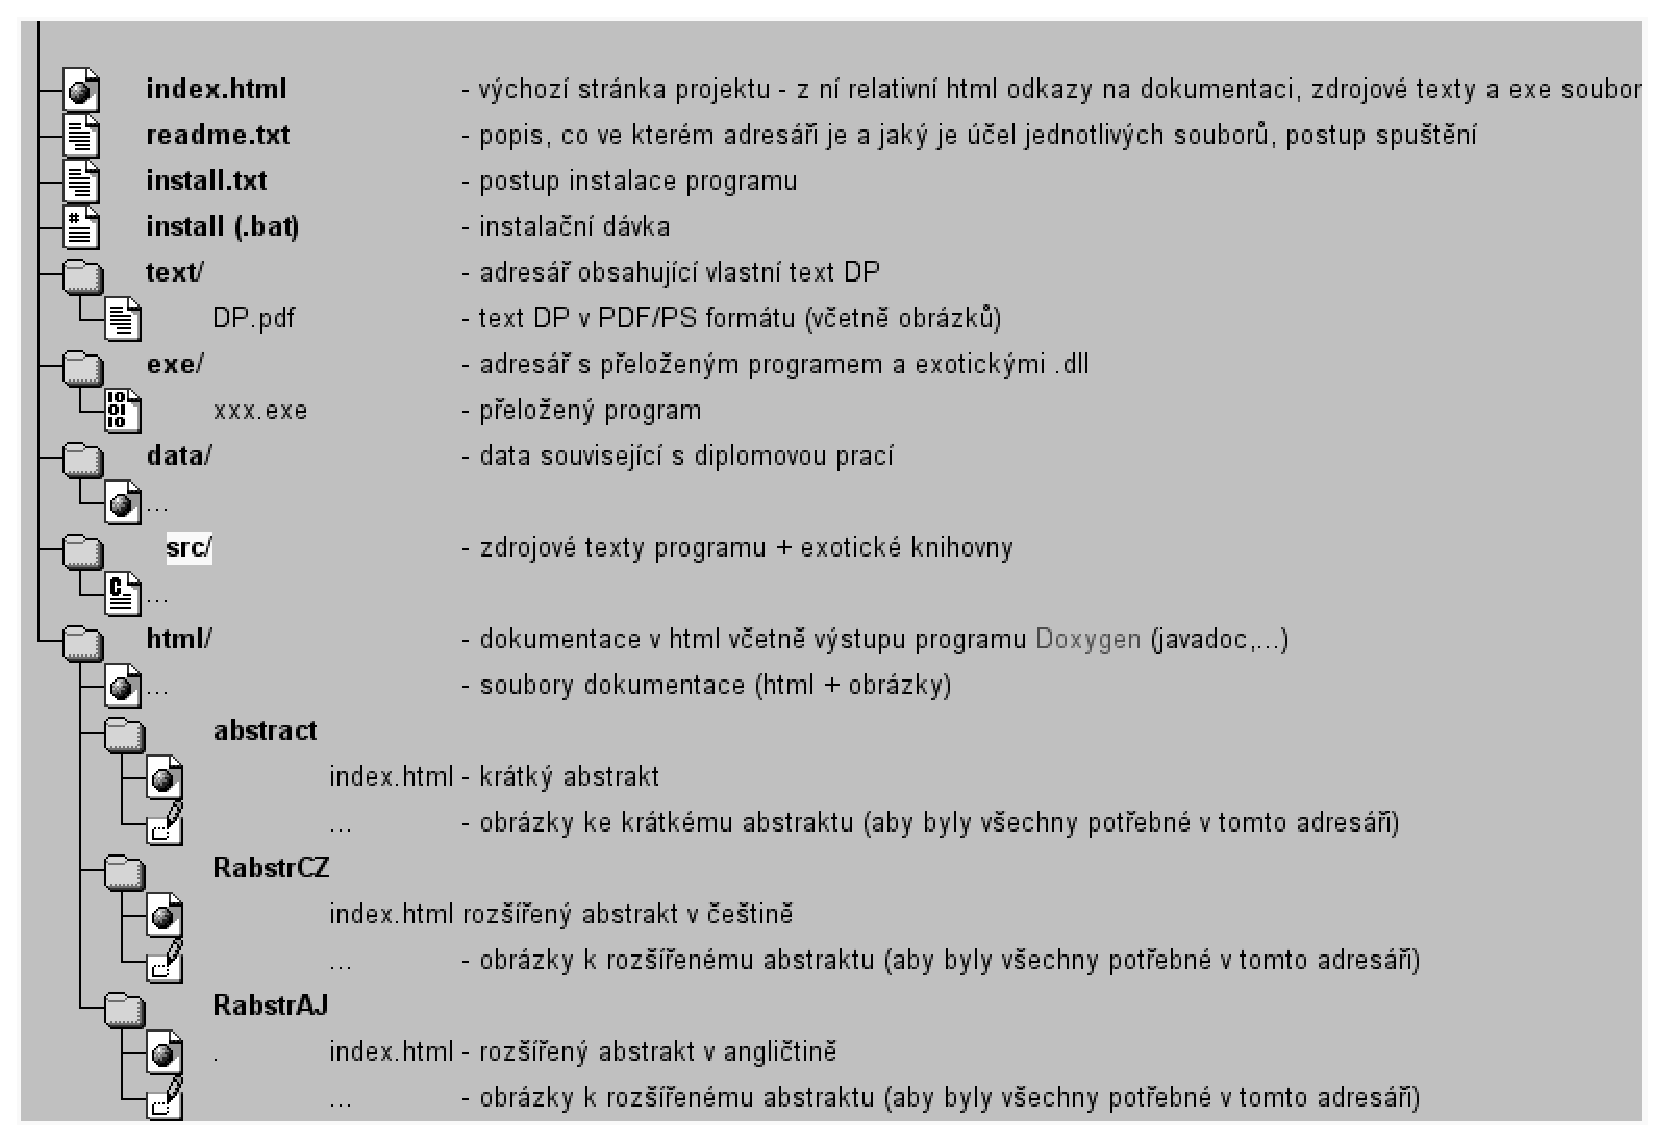
\includegraphics[width=14cm]{figures/seznamcd}
\caption{Seznam přiloženého CD --- příklad}
\label{fig:seznamcd}
\end{center}
\end{figure}

Na GNU/Linuxu si strukturu přiloženého CD můžete snadno vyrobit příkazem:\\ 
\verb|$ tree . >tree.txt|\\
Ve vzniklém souboru pak stačí pouze doplnit komentáře.

Z \textbf{README.TXT} (případne index.html apod.)  musí být rovněž zřejmé, jak programy instalovat, spouštět a jaké požadavky mají tyto programy na hardware.

Adresář \textbf{text}  musí obsahovat soubor s vlastním textem práce v PDF nebo PS formátu, který bude později použit pro prezentaci diplomové práce na WWW.



\end{document}
